\chapter{Detector Response to $^{14}$C Beta Decay}

The carbon-14 calibration follows the same preparation and injection procedure as the tritium calibration, which has been described in previous papers\cite{lux_tritium,richard,attila}. Both of these calibration sources have half-lives greater than the lifetime of the experiment, so we rely on the LUX gas processing system to chemically remove the injected activity. We have previously characterized our ability to remove radio-labelled methane from the LUX detector and found that tritiated-methane (CH$_3$T) is removed with a decay time of about 7-10 hours, leaving no observed residual activity in the detector. Carbon-14 labelled methane ($^{14}$CH$_4$) is chemically identical to CH$_3$T and so we find it to have the same removal characteristics. The tritiated methane is removed with a time constant of 8.2 hours, and the carbon-14 labeled methane is removed with a time constant 9.1 hours. This variation in removal time is within reason given the variation in previous trials with tritiated methane.
\begin{figure}[h!]
\centering
\begin{subfigure}{0.5\textwidth}
  \centering
  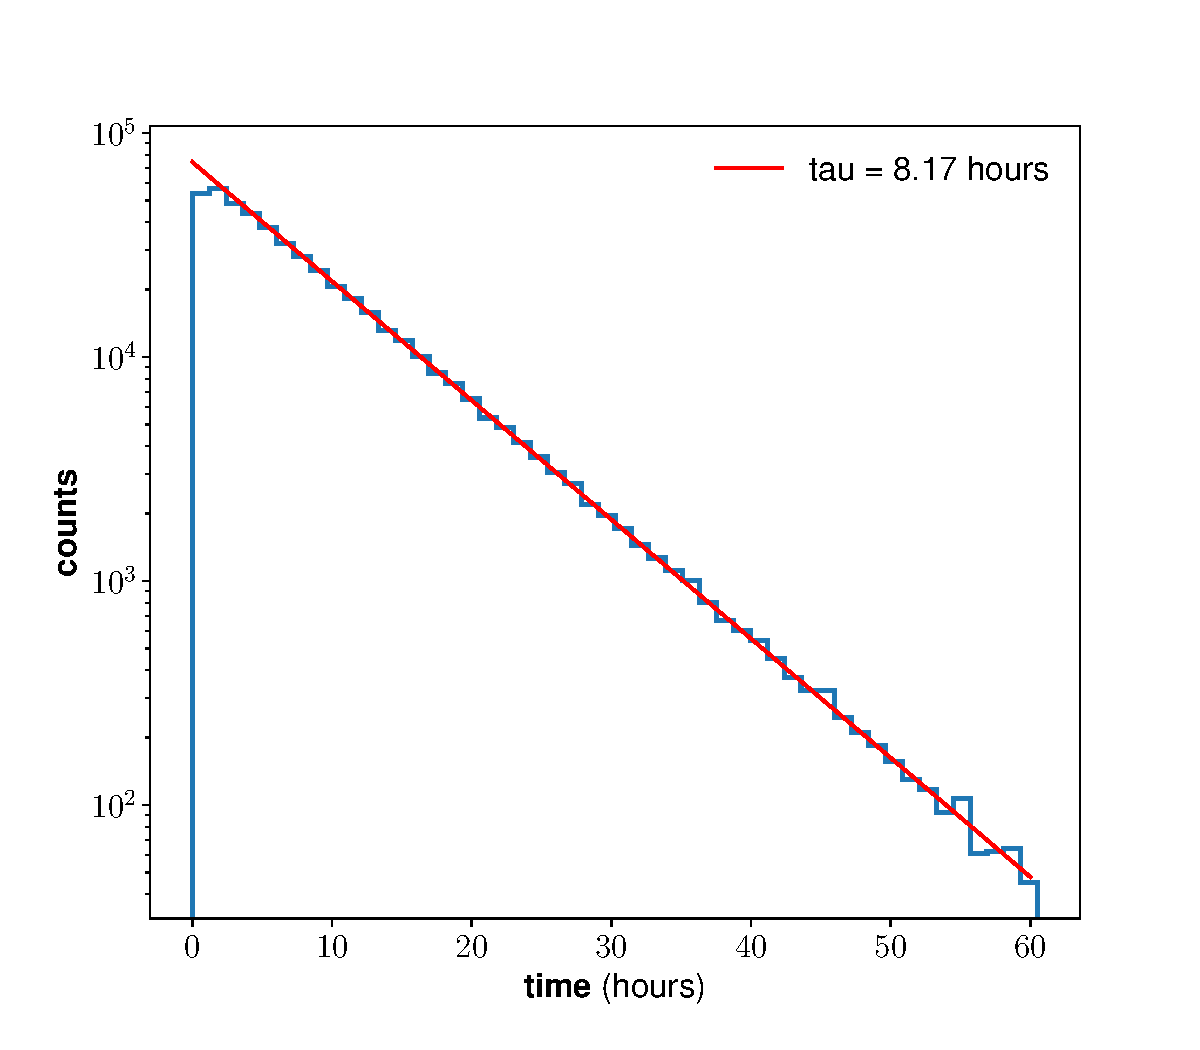
\includegraphics[width=\textwidth]{Figures/H3_removal_time.pdf}
  %\label{}
\end{subfigure}%
\begin{subfigure}{0.5\textwidth}
  \centering
  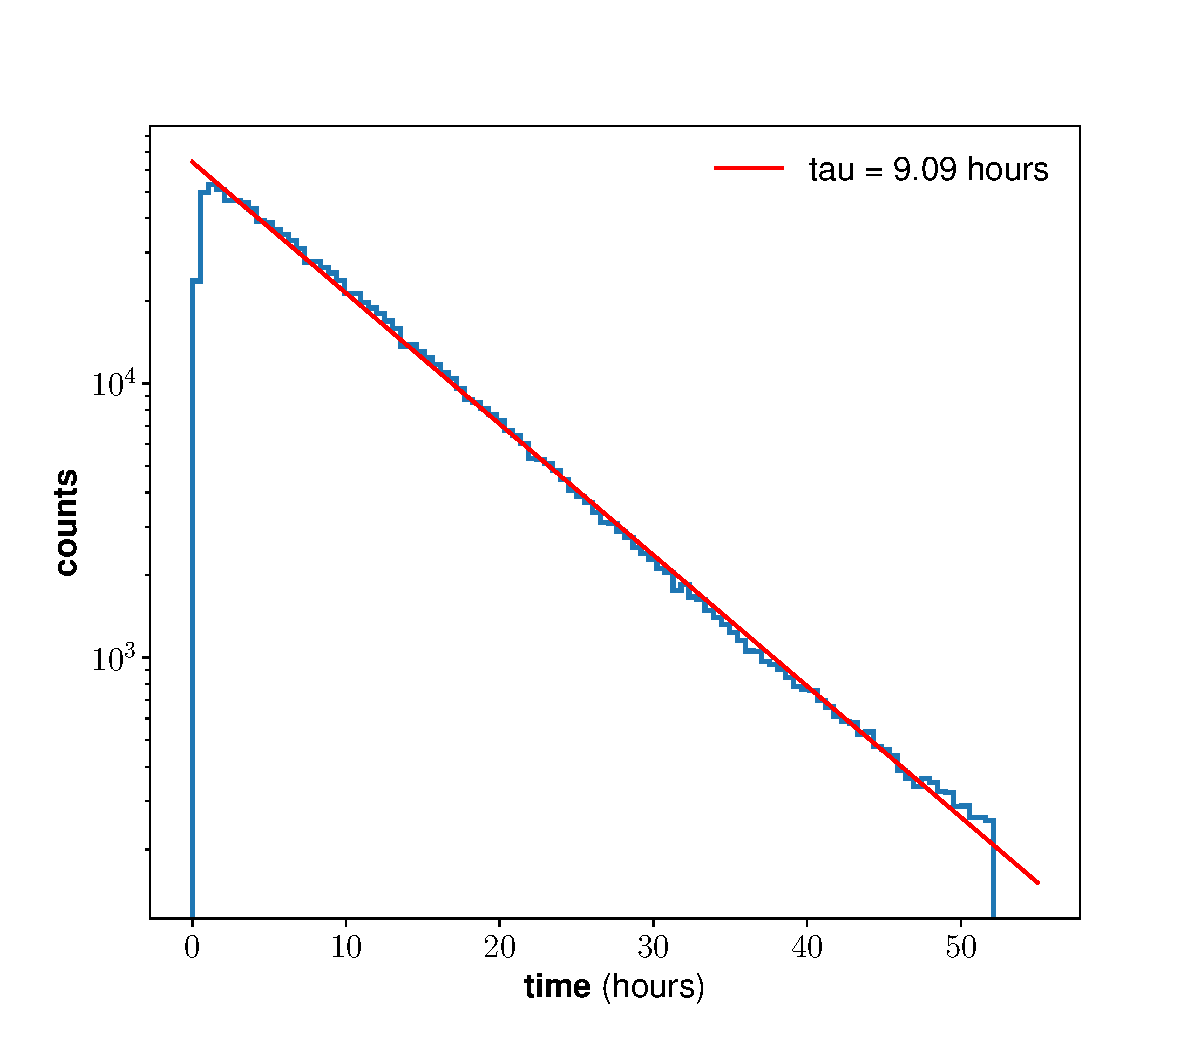
\includegraphics[width=\textwidth]{Figures/C14_removal_time.pdf}
  %\label{fig:intlin}
\end{subfigure}
\caption{Purification of methane radio-labeled with tritium (left), and carbon-14 (right). The tritiated methane is removed with a time constant of 8.2 hours, and the carbon-14 labeled methane is removed with a time constant 9.1 hours. }
\label{fig:removaltime}
\end{figure}




The endpoint of the carbon-14 spectrum is obscured by the xenon-131m line. We don not assume that gammas and betas behave in the same way in liquid xenon, so we need to cut out the xenon-131m events in order to measure the energy deposition properties of carbon-14. At 145 keV, the xenon distribution falls to less than 5\% of the carbon-14 distribution, so we will only include events with reconstructed energy $<145$ keV in our measurement of the carbon-14 yields and recombination..
\begin{figure}[h!]
\centering
  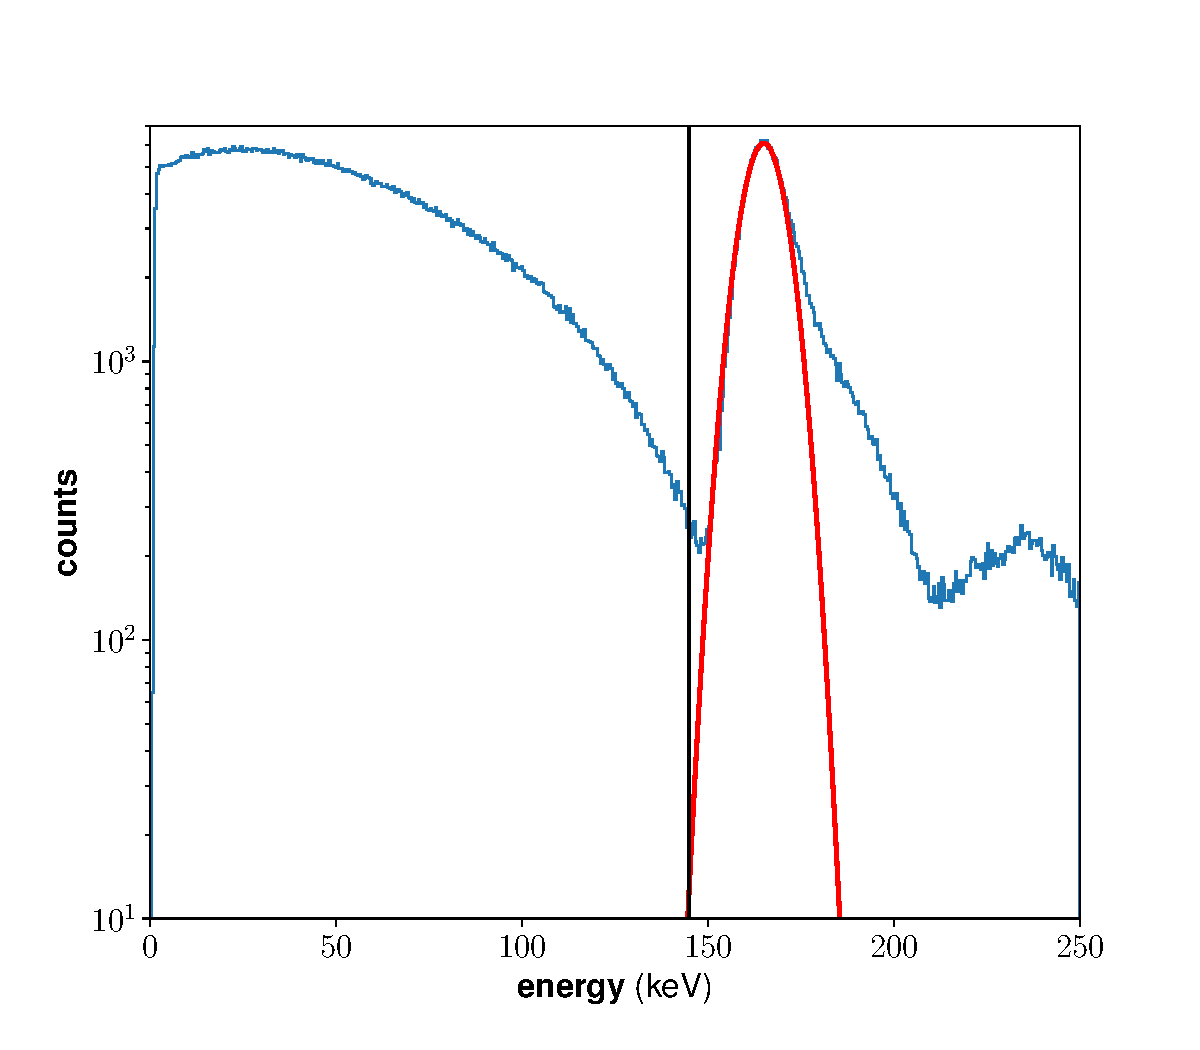
\includegraphics[width=\textwidth]{Figures/C14_spec_init.pdf}
\caption{Reconstructed energy spectrum of the carbon-14 calibration. The blue histogram was generated using all of the events in the dataset, including both carbon-14 and Xe-131m. Most of the events are in the smooth carbon-14 beta spectrum, which extends from 0 to 156 keV, but the Xe-131m line is clearly visible at 164 keV. The red curve shows a Gaussian fit to the xenon-131m spectrum, excluding the high energy side. The black line shows our energy cut at 145 keV.}
\label{fig:c14Ecut}
\end{figure}



\section{The Theoretical $^{14}$C Beta-Spectrum}
The shape of the theoretical spectrum of the carbon-14 beta decay has been of interest in the context neutrino mass experiments\cite{C14_Wietfeldt}, where the goal is to measure the precise endpoint, and in liquid scintillator experiments, which have $^{14}$C as a major background and so need to model the spectrum with high precision\cite{C14_Borexino, C14_Bergeron}. This  decay also is of interest in theoretical nuclear physics because it has an abnormally long half life\cite{C14_Kuzminov,C14_Genz,C14_Garcia}. The transition of $^{14}$C to the ground state of $^{14}$N is an allowed Gamow-Teller $(0^+ \rightarrow 1^+)$ transition. The 5730 year half-life, and corresponding comparative half life, $\log_{10}(f_t)=9.04$, makes it empirically consistent with second-forbidden transitions\cite{C14_Kuzminov,C14_Wietfeldt}.

This extended half life indicates an anomalously small Gamow-Teller nuclear matrix element of $\langle GT \rangle \approx 2 \times 10^{-3}$. This points to cancellation in the lowest order terms of the nuclear matrix element and means that higher order terms must be taken into consideration. These higher-order terms may introduce momentum-dependent deviations from the allowed spectral shape. There have been several experiments\cite{C14_Sonntag, C14_Wietfeldt, C14_Borexino, C14_Kuzminov, C14_Bergeron} which have made measurements of the spectral shape which are consistent with non-statistical corrections to the allowed shape. These results are in some tension with each other, as well as with previous measurements which show a purely allowed spectral shape\cite{C14_Curran}. 

\subsection{The Allowed Spectrum}
Carbon-14 decays to the ground state of nitrogen-14 by way of an allowed Gamow-Teller, 0$^+$ to 1$^+$ transition. This decay has a Q-value of 156 keV and a half life of 5730 years. In general, the theoretical spectrum for this decay takes the form\cite{C14_Kuzminov}:
\begin{equation}\label{eq:beta_spec}
\frac{dN}{dE}=\frac{1}{2\pi^3} \xi C(E) F(Z,E) pE(E_0-E)^2
\end{equation}
Here, $p$ and $E$ are the momentum and total energy of the emitted beta, and $E_0$ is the endpoint energy of the spectrum. In equation \ref{eq:beta_spec} we have neglected the neutrino mass as well as a radiative correction term which is expected to have $<1\%$ effect on the shape of the spectrum\cite{C14_Wietfeldt}. The initial distribution of momentum between the electron and neutrino is proportional to $pE(E_0-E)^2$. This is derived by the phase space density of free particles and will be referred to as the phase space factor. The Fermi function $F(Z,E)$ contains information about the interaction between the emitted beta and the daughter nucleus. The terms $\xi$ and  $C(E)$ represent the energy independent and energy independent parts of the nuclear matrix element.

\subsection{The Fermi Function}\label{sec:fermifunc}
As the emitted beta travels away from the daughter nucleus, the two interact and either increase or decrease the momentum of the beta, depending on its charge. In the case of $^{14}C$, the beta has a negative charge and has to climb up out of the electric potential created by the $^{14}N$ daughter nucleus. The resulting observed beta spectrum will then be pulled to lower energy than the initial phase space factor. This modification to the spectrum if known as the Fermi function, $F(Z,E)$. The traditional derivation of $F(Z,E)$ begins by assuming the daughter nucleus is a fixed point charge and then evaluates the electron wave-function given the resulting field. The wave function is only evaluated down to the nuclear radius, $R$, in order to avoid divergence\cite{wilkinson}:
\begin{equation}\label{eq:fermifunc1}
F(Z,E)=2(\gamma+1)\Gamma(2\gamma+1)^{-2}(2pR)^{2(\gamma-1)}e^{\pi \alpha Z E/p}|\Gamma(\gamma+i\alpha ZE/p)^{2}|^2
\end{equation}

There is also a much simpler closed-form solution in the low-Z, non-relativistic approximation\cite{beta_fermi}:
\begin{equation}\label{eq:fermifunc2}
F_{NR}(Z,E)=\frac{x}{1-exp(-x)},
\end{equation}
where $x=2\pi Ze^{2}/\hbar v$. Here, $Z$ is the atomic number of the daughter nucleus, $e$ is the electron charge, and $v$ is the final velocity of the beta particle. 

Electrons in the higher-momentum part of the spectrum will have velocities exceeding 0.5c, so the non-relativistic approximation may not hold. This being the case, we consider the Bethe-Bacher approximation, which estimates the relativistic correction\cite{beta_fermi,bethe}:
\begin{equation}\label{eq:fermifunc3}
F_{BB}(Z,E)=F_{NR}(Z,E)[W^2(1+4\gamma^2)-1]^S,
\end{equation}
where $W\equiv E/m_ec^2$, $\gamma \equiv \alpha Z$, and $S\equiv (1-\gamma^2)^{1/2}-1)$. The full relativistic Fermi function can be estimated by a series expansion on powers of $(\alpha Z)$\cite{wilkinson,C14_Wietfeldt}. This sum is of limited use to us here because it becomes invalid at low kinetic energy and in fact diverges at zero.

The final correction to the Fermi function we consider is the correction for screening of the Coulomb potential by the orbital electrons. This essentially amounts to a shift in the origin of $F(Z,E)$\cite{C14_Wietfeldt,beta_screening}:
\begin{equation}\label{eq:fermifunc4}
F_{S}(Z,E)=\frac{E'p'}{Ep}F(Z,E'),
\end{equation}
where $E'=E-V_0$ and $p'$ is is the associated momentum. For the $^{14}$C beta decay, $V_0=495$eV\cite{C14_Wietfeldt}.

Figure \ref{fig:C14_spec_corrs} compares the non-relativistic approximation to the various corrections described in this section. We can see that the Wilkinson expansion differs from $F_{NR}(7,E)$ by less than a percent down to a few eV, at which point it diverges. The Bethe-Bacher approximation is similarly very close to $F_{NR}(7,E)$, but it does not display the same pathological behavior at the origin. The correction for electron screening peaks at 1.5\% at a kinetic energy of $T=3.5$keV. Because of the pathology in the Wilkinson expansion, we will take our Fermi function to be the combination of equations \ref{eq:fermifunc3} and \ref{eq:fermifunc4}:
\begin{equation}\label{eq:fermifunc5}
F(Z,E)=\frac{E'p'}{Ep}F_{NR}(Z,E')[(E'/m_ec^2)^2(1+4\gamma^2)-1]^S,
\end{equation}
with $F_{NR}(Z,E)$ as defined in equation \ref{eq:fermifunc2} and $E'$ and $p'$ as defined for eqaution \ref{eq:fermifunc4}.

\begin{figure}[h!]
\centering
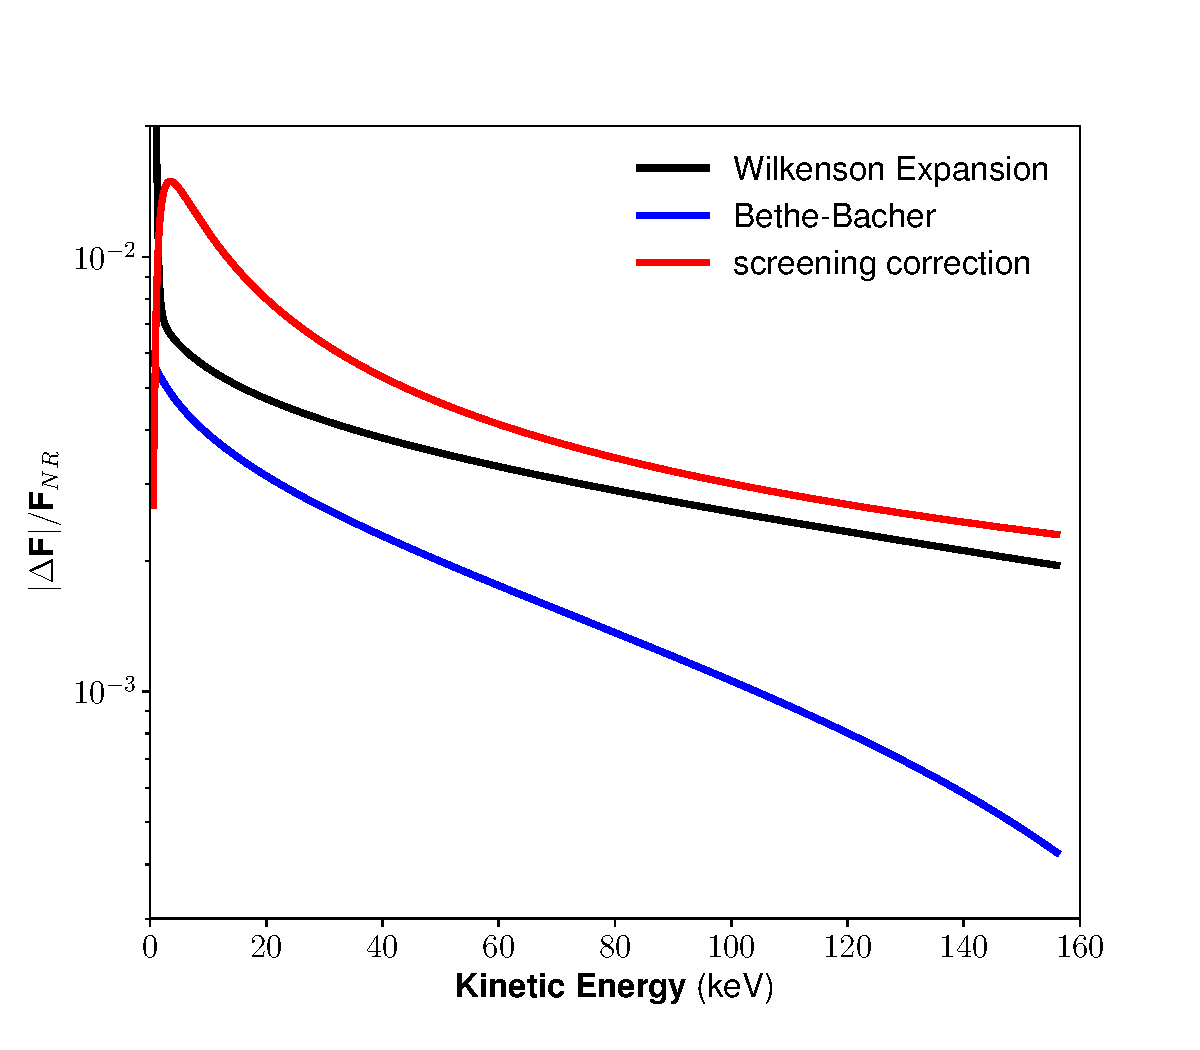
\includegraphics[width=\textwidth]{Figures/FermiFunc_compare.pdf}
\caption{Correction factors for the $^{14}$C beta Fermi function. We compare the non-relativistic approximation, $F_{NR}(7,E)$ to the relativistic corrections described in section \ref{sec:fermifunc}, as well as the non-relativistic function after having been adjusted to account for screening by the orbital electrons. Plotted is $|F'(7,E)-F_{NR}(7,E)|/F_{NR}(7,E)$, where $F'(7,E)$ are the adjusted Fermi functions as indicated in the legend.} 
\label{fig:C14_spec_corrs}
\end{figure}

\subsection{The Shape Factor}\label{sec:shape_factor}
For a typical allowed decay, the shape factor is dominated by interference between the Gammow-Teller axial matrix element, $\langle GT \rangle$ and the weak magnetism matrix element, $\langle WM \rangle$. Such a shape factor has the form\cite{C14_Kuzminov,C14_Garcia,C14_Wietfeldt,beta_Calaprice}:
\begin{equation}\label{eq:shapefactor1}
C(E)\approx1+\frac{4}{3M}\frac{\langle WM \rangle}{\langle GT \rangle}[E-E_0/2-m_e^2/E],
\end{equation}
where $M$ is the nucleon mass, $m_e$ is the electron mass, and $E_0$ is the endpoint energy of the beta-spectrum. Usually the energy dependence of $C(E)$ is small enough that it can be neglected, but in the $^{14}$C beta decay the suppressed decay rate means that $\langle GT \rangle$ is small enough to make its consideration necessary. Under the conserved vector current hypothesis (CVC), the weak magnetism matrix element can be analogized to that of an M1 electromagnetic transition ($\langle WM \rangle$=$\langle M1 \rangle$) for the purpose of calculating the expected shape factor. The ground state of $^{14}$C is an element of an isospin triplet, together with the $^{14}$O ground state and the first excited state of $^{14}$N. The M1 transition is the same as that of the first excited state of $^{14}$N transitioning to the ground state.

There have been several calculations of the predicted shape factor\cite{C14_Garcia,C14_Wietfeldt,C14_Genz}. These typically use a more general form of the $C(E)$ which takes into account terms which have been neglected from equation \ref{eq:shapefactor1}:
\begin{equation}\label{eq:shapefactor2}
C(E)=1+aE+\mu_1\gamma_1b/E+cE^2,
\end{equation}
where $\gamma_1=[1+(\alpha Z)^2]^{1/2}$ and $\mu_1$ is a special Coulomb function. The coefficients $a$, $b$, and $c$ can be calculated using the appropriate matrix elements. The matrix elements are typically calculated using model wave functions for the $^{14}$C and $^{14}$N ground states.

The first measurement of the $^{14}$C shape factor was made by Sonntag et. al. in 1970\cite{C14_Sonntag}. In units of MeV, his measured shape factor was, $C(E)=1-9.14E+1.53/E+7.66E^2$. Genz et. al.\cite{C14_Genz} used this result in part to derive phenomenological wave functions which replicate the shape factor. Later experiments and theoretical calculations have rejected this shape factor.

Wietfeldt et. al. found their data to be consistent with a shape factor of $C(E)=1+aE$, with $a=-0.45 \text{ \ MeV}^{-1}$\cite{C14_Wietfeldt}. This result is very close to their own theoretical calculation of $a=-0.38 \pm 0.04 \text{ \ MeV}^{-1}$, along with theoretical calculations by Garcia and Brown\cite{C14_Garcia}, and  Calaprice and Holstein\cite{beta_Calaprice}. However, the best-fit value of $a$ was inconsistent depending on what range of energies was fit, and a second measurement of the spectrum 2 years later yielded a best fit parameter of $a=-0.63 \pm 0.05 \text{ \ MeV}^{-1}$. 

The Borexino collaboration attempted to measure the shape of the $^{14}$C beta spectrum using their counting test facility (CTF). They assumed the same functional form as the Wietfeldt paper and excluded all $a<-0.72 \text{ \ MeV}^{-1}$ with 90\% confidence\cite{C14_Borexino}. 


Most recently, V. Kuzminov and N. Osetrova measured the shape factor of then $^{14}$C beta decay using a wall-less proportional counter\cite{C14_Kuzminov}. They assumed a shape factor with the form, $C(E)=1+\beta(Q-T)$, with $Q$ being the endpoint energy and $T$ being the kinetic energy of the electron. They measured $\beta=1.24 \pm0.04 \text{ \ MeV}^{-1}$, which is in agreement with a theoretical calculation by Genz et. al.\cite{C14_Genz}. This result is equivalent to $a=-0.68 \pm0.02 \text{ \ MeV}^{-1}$ in a Wietfeldt-style shape factor and is very close to both the Borexino measured limit, as well as the second Wietfeldt measurement.

\begin{figure}[h!]
\centering
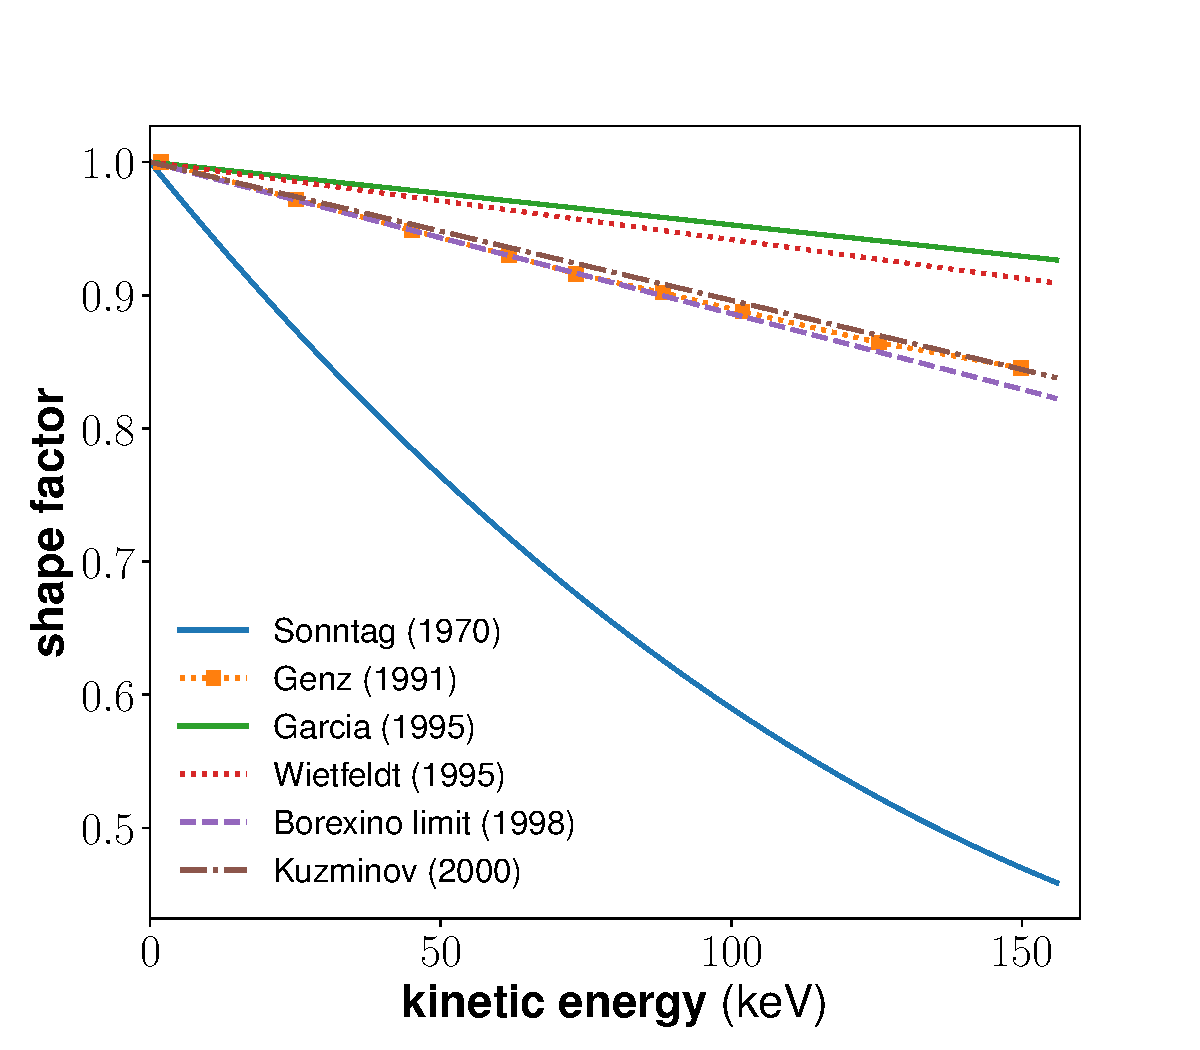
\includegraphics[width=\textwidth]{Figures/ShapeFac_compare.pdf}
\caption{Various measurements and theoretical calculations of the $^{14}$C shape factor. They have all been normalized to equal 1 at kinetic energy=0 keV. The Sonntag\cite{C14_Sonntag}, Wietfeldt\cite{C14_Wietfeldt}, Borexino\cite{C14_Borexino}, and Kuzminov\cite{C14_Kuzminov} lines are all experimental measurements, while the Genz\cite{C14_Genz} and Garcia\cite{C14_Garcia} lines are theoretical calculations. It is clear that the Sonntag result is strongly disfavored by all subsequent experiments and theoretical calculations. This figure also shows Genz, Borexino, Kuzminov, as well as the second Wietfeldt result (not shown) all converging around $C(E)\approx 1-(0.7 \text{ \ MeV}^{-1})E$. It would be difficult, however, to claim this as consensus because the only true measurement in this subset is the Kuzminov line. Neither the Borexino paper nor the Wietfeldt paper claim a strong measurement of the shape factor.} 
\label{fig:C14_shape}
\end{figure}



\section{Accounting for Finite Detector Resolution}\label{sec:desmearing}
The carbon-14 injection was based on the tritium calibration, which was first performed in August of 2013, after the first LUX data run was completed. The data from this calibration was used to calculate the energy deposition properties of electronic recoils in liquid xenon. To this end, a method was developed by Attila Dobi which deconvolved the effects of detector-resolution from the interesting physics involved in the process\cite{lux_tritium,attila}. 


\subsection{Gaussian Energy Resolution and Continuous Beta Spectra}
This deconvolution of detector resolution is necessary because of the continuous nature of beta spectra. We do not know the true deposition energy, $E_{true}$, of any given event and only have access to the reconstructed energy, $E_{rec}=W\left(n_{\gamma}+n_{e}\right)$, where $n_{\gamma}\equiv \frac{S1_c}{G1}$ and $n_{e}\equiv \frac{S2_c}{G2}$, where the subscript ``c'' indicates an efficiency-corrected value. In the Run03 measurements, the reconstructed energy of any event would be drawn from a Gaussian distribution centered at the true deposition energy, with the width of this distribution being the energy resolution, $\sigma_{E}$. 
\begin{figure}[h!]
\centering
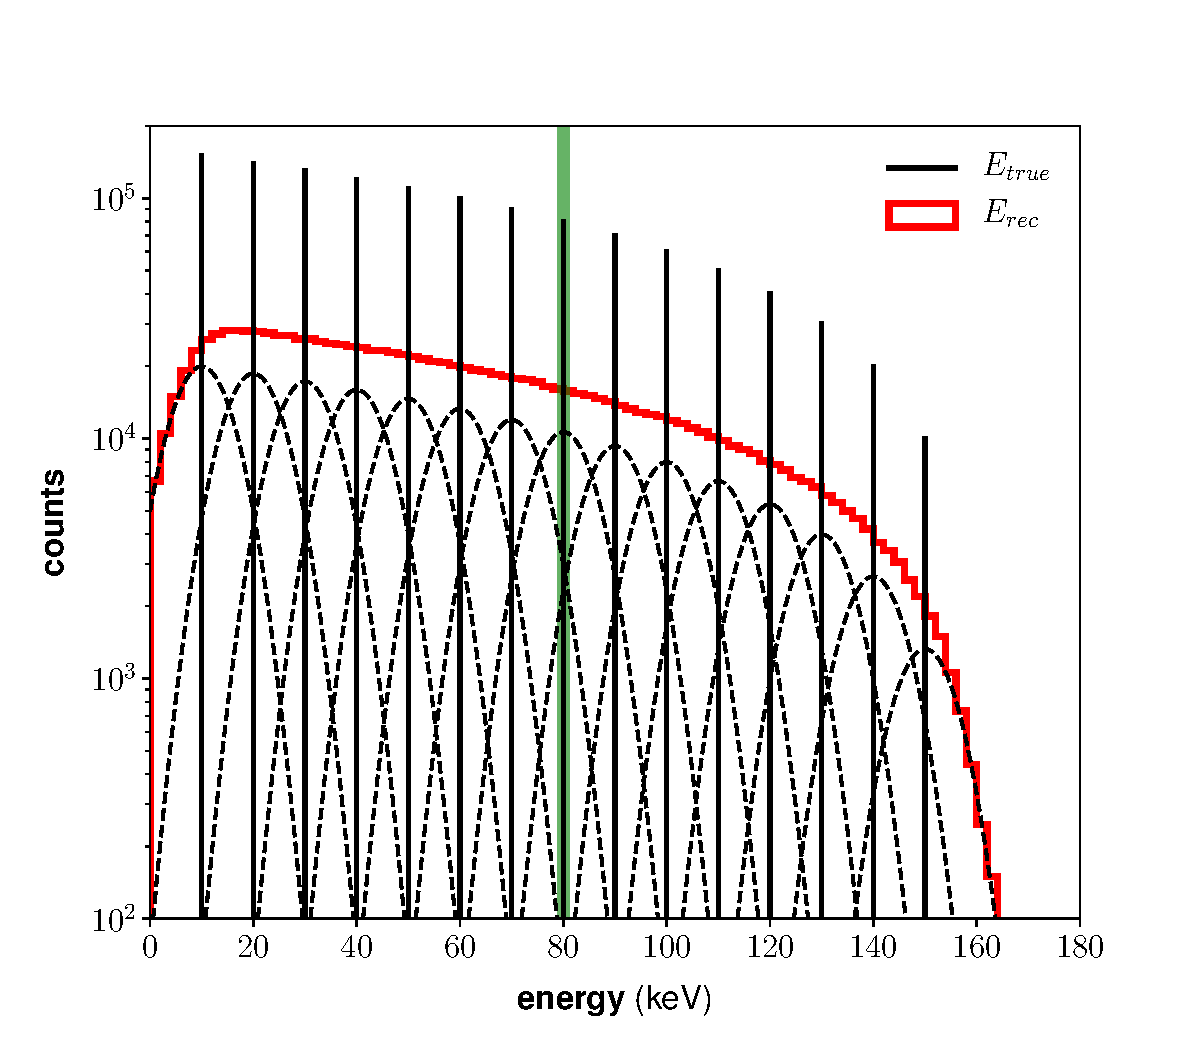
\includegraphics[width=\textwidth]{Figures/toy_smearing.pdf}
\caption{Smearing of a discrete, linearly falling spectrum. The true energy of the events is distributed at ( 10, 20, 30, ... ,150 ) keV, as indicated by the solid black lines. The number of events at each energy decreases linearly. We then apply Gaussian smearing with a flat resolution of 6 keV to the true energy (dashed lines). The reconstructed energy (red histogram) shows the resulting spectrum. The average true energy of events in a slice from 79.75 keV $<E_{rec}<$ 80.25 keV (green area) is 70.65 $\pm$0.09 keV. This average is offset from the selected energy due to smearing.}
\label{fig:toysmear}
\end{figure}

When this Gaussian smearing is applied to a continuous spectrum with a non-zero slope, it will create a systematic offset the measured reconstructed energy from the true energy. We take the spectrum shown in figure \ref{fig:toysmear} as an example. The true energy of the events is distributed at discrete energies, 10, 20, 30, up to 150 keV. We apply Gaussian smearing with a constant resolution of $\sigma_{E}$= 6 keV to give us our reconstructed energy spectrum. When we take a small slice in reconstructed energy, from 79.75 to 80.25 keV, we find that the average true energy of events in this slice is systematically offset to 79.53 $\pm$0.09 keV. This offset is due to the negative slope of the true energy spectrum. The lower energy bins are more prominent than the higher energy ones, and therefore will have more events smear into our reconstructed energy slice.

It is possible to calculate this offset explicitly by integrating the contribution from each individual Gaussian. The number of events contributed to our reconstructed energy slice by the $i^{th}$ true energy bin will be given by:
\begin{equation}\label{eq:smear1}
\begin{split}
A_{80,i}&=\int_{79.75}^{80.25}N_iG(x;E_{true,i},\sigma_E)dx\\
&=\int_{79.75}^{80.25}\frac{N_i}{\sqrt{2\pi \sigma_{E}^{2}}} \exp \left(\frac{-(x-E_{true,i})^2}{2\sigma_{E}^{2}}\right)dx\\
&=\frac{N_i}{2} \Bigg(\text{erf} \bigg(\frac{80.25-E_{true,i}}{\sqrt{2\sigma_E^2}}\bigg)-\text{erf} \bigg(\frac{79.75-E_{true,i}}{\sqrt{2\sigma_E^2}}\bigg)\Bigg)
\end{split}
\end{equation}
where, $N_i=C(16-i)$ is the number of events generated for  the $i^{th}$ discrete energy, and $C$ is a scaling constant. The expected mean true energy, $\nu_{80}$, of events in the slice will then be given by:
\begin{equation}\label{eq:smear2}
\nu_{80}=\frac{\sum_i E_{true,i}A_{80,i}}{\sum_i A_{80,i}}
\end{equation}
For the stated values of $N_i$, $E_{true,i}$, and $\sigma_E$, equation \ref{eq:smear2} yields $\nu_{80}=79.56$ keV, which is consistent with the result found in the previous paragraph.  

Equation \ref{eq:smear1} can be used to recenter an arbitrary reconstructed energy bin. This correction will be most important for energy regions where the spectrum in question is steeply changing and at its endpoints. For instance, if we take a reconstructed energy slice of our toy spectrum from 149.75 to 150.25 keV, the predicted low-energy bias goes from 0.44 keV as it was for the 80 keV slice, to 3.5 keV. This prediction is consistent with the measured bias of 3.4 $\pm$0.2 keV.

We can generalize equations \ref{eq:smear1} and \ref{eq:smear2} to apply to decays with continuous energy spectra. If the energy resolution of the detector, $\sigma_E(E)$, and the shape of the spectrum, $\frac{dN}{dE}$, are both known, equations \ref{eq:smear1} and \ref{eq:smear2} can be rewritten:
\begin{equation}\label{eq:smear3}
A(E;E_1,E_2)=\frac{1}{2}\frac{dN}{dE} \Bigg(\text{erf} \bigg(\frac{E_2-E}{\sqrt{2\sigma_E(E)^2}}\bigg)-\text{erf}\bigg(\frac{E_1-E}{\sqrt{2\sigma_E(E)^2}}\bigg)\Bigg),
\end{equation}
and:
\begin{equation}\label{eq:smear4}
\nu(E_1,E_2)=\frac{\int A(E,E_1,E_2)EdE}{\int A(B_1,B_2)dE},
\end{equation}
where $E_1$ and $E_2$ are the edges of the reconstructed energy slice. The calculated $\nu(E_1,E_2)$ can then be used to recenter the arbitrary reconstructed energy bin to the average true energy of events in that bin.

\subsection{Gaussian Smearing in the Combined Energy Model}
In the previous section, we presented a method for calculating the average true energy, $\nu(E_1,E_2)$, of beta-events in a reconstructed energy bin, given precise knowledge of the beta-decay spectrum and detector resolution. The question remains whether the events within that bin are representative of its average true energy. Specifically, we would like to derive a relationship between the average number of photons and electrons measured from events in the bin ($\langle n_{\gamma}\rangle_i$ and $\langle n_{e} \rangle_i$) and the average number of photons and electrons that would be produced by a mono-energetic decay located at $\nu(E_1,E_2)$ ($\langle N_{\gamma} \rangle_{\nu}$ and $\langle N_{e} \rangle_{\nu}$). 

There are many factors to take into account when considering this question. First, we would again need to know the shape of the beta spectrum. In addition to the combined energy resolution, we also need knowledge of the individual electron and photon resolutions, which we will define as $\sigma_{e,det}$ and $\sigma_{\gamma,det}$ respectively. We also need to consider the energy-dependent charge yield ($QY\equiv \langle N_{e} \rangle/E_{true}$) and light yield ($LY\equiv \langle N_{\gamma} \rangle/E_{true}$), as well as the size of the fluctuations in the recombination process, $\sigma_R$. 
\begin{figure}[h!]
\centering
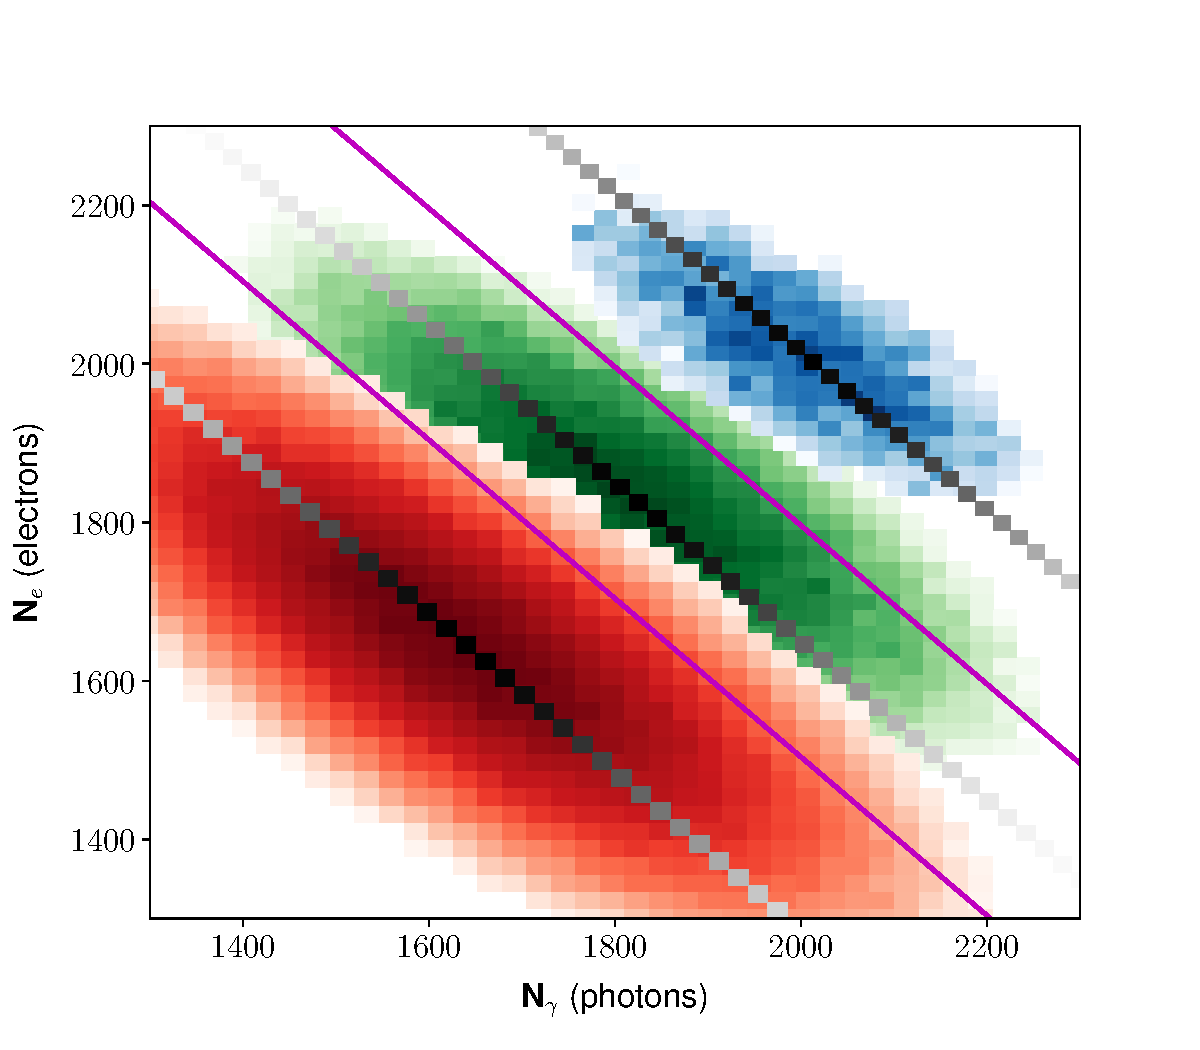
\includegraphics[width=\textwidth]{Figures/toy_smearing_2d_Rflat.pdf}
\caption{Detector resolution applied to a toy spectrum using the combined-energy model. Events are generated at 45 (red), 50 (green), and 55 (blue) keV. The greyscale diagonals indicate smearing along lines of constant energy. The blue, green, and red populations show the distribution of events after detector resolution is modeled.}
\label{fig:toysmear2d}
\end{figure}

In figure \ref{fig:toysmear2d} we have applied detector resolution to a toy spectrum comprised of 3 discrete energies, 45, 50, and 55 keV. We simulate a steeply falling spectral shape by distributing the events in a ratio of (4:2:1) between the stated energies. We calculate $\langle N_{\gamma} \rangle$ and $\langle N_{e} \rangle$ using a constant electron fraction, $y\equiv \frac{\langle N_{e} \rangle}{E_{true}/W}=0.5$, where the work function, $W=1/73$. We apply recombination fluctuations with a magnitude of $\sigma_R$=214.3 quanta, which is the predicted value for a 50 keV decay from \cite{attila}. This gives $N_{e}=N(\langle N_{e} \rangle,\sigma_R)$ and $N_{\gamma}=E_{true}/W-N_{e}$, where $N(\mu,\sigma)$ is a random normal distribution. To produce the measured values of $n_e$ and $n_{\gamma}$, we apply electron and photon resolutions of $\sigma_{e,det}=1\cdot \sqrt{N_{e}}$ and $\sigma_{\gamma,det}=4\cdot \sqrt{N_{\gamma}}$, which are roughly characteristic of the LUX detector. 

We investigate the effect of detector resolution on this toy spectrum by selecting events that fall between 48 and 52 keV in reconstructed energy. As expected from the previous section, the average true energy, $\nu(48,52)=49.24 \ \pm 0.08$ keV, has a downward biased from 50 keV. This is consistent with predictions from the previous section. 

An important observation to make here is that $\sigma_R$ is expected to be correlated with $\sigma_{e,det}$ and $\sigma_{\gamma,det}$. Consider two events from the 50 keV population, one with $N_{e}=\langle N_{e} \rangle+\sigma_R$ and one with $N_{e}=\langle N_{e} \rangle-\sigma_R$. The first event would have about 27\% more electrons than the second, while the second event would have about 27\% more photons than the first. Taking into account the dependence of $\sigma_{e,det}$ and $\sigma_{\gamma,det}$ on $N_{e}$ and $N_{\gamma}$ we find that the second event would have a 19\% larger combined energy resolution than the first. Events drawn from the 50 keV population will therefore be biased to lower values of $n_{\gamma}$ and higher values of $n_e$ because the population is narrower and therefore more dense in this region. In our toy model look at events from the 50 keV population that are selected by our reconstructed energy slice and find that the average $N_{\gamma}$ of these events is $1816 \ \pm3$ photons, while the true mean of $N_{\gamma}$ for events in the 50 keV population is 1825 photons. The opposite effect is seen when looking at $N_{e}$, whose mean is $1833 \ \pm3$ electrons for binned events. 

This bias will be offset, at least to some degree by an opposing effect on the 45 and 55 keV populations. These populations will also be wider at high values of $N_{\gamma}$, and so our reconstructed energy slice will select more events from these regions than from the associated low-$N_{\gamma}$ regions. In our slice we find that the 45 keV line contributes events with an average $N_{\gamma}$ of $1770 \ \pm5$ photons. This is compare to the true average of 1642.5 photons. Similarly, the 55 keV line contributes events with an average $N_{\gamma}$ of $2027 \ \pm12$ photons, compared to its true average of 2007.5 photons.

For the model we have described, it turns out that all of the competing effects on $N_{\gamma}$ and $N_{e}$ cancel out, and the averages for events in our reconstructed energy slice are consistent with what is expected for the measured value of $\nu(48,52)=49.24 \ \pm 0.08$ keV. The expected ($N_{\gamma}$,$N_{e}$) for a decay with energy $49.24 \ \pm 0.08$ is (1797,1797) $\pm$(3,3) quanta, while the observed values were (1799,1796) $\pm$(3,3) quanta. The effects also cancel for a slice centered at 55 keV, but a small offset of 7 $\pm$3 quanta is observed in a slice at 45 keV. 

We also modified the model to allow for a changing electron-fraction. We set $y=$ 0.52, 0.5, and 0.48 for the 45, 50, and 55 keV populations, respectively. With this modified model, the observed averages in the 50 and 55 keV bins are no longer consistent with what is expected from the measured $\nu$. This indicates that any smearing correction to be applied to map ($\langle n_{\gamma}\rangle,\langle  n_{e}\rangle$) to ($\langle N_{\gamma}\rangle,\langle N_{e}\rangle$) will be largely determined by the energy dependence of electron and photon yields. 
\begin{table}[h!]
\centering
    \begin{tabular}{ c | c | c | c | c | c | c | c | c | c }
    \hline
    $E_{rec,i}$ (keV) & $\nu$ (keV) & $\pm$ & $\langle N_{\gamma} \rangle_{i}$  & $\langle N_{\gamma} \rangle_{\nu}$ & $\pm$ & $\langle N_{\gamma} \rangle_{obs}$ & $\pm$ & $\langle n_{\gamma} \rangle$ & $\pm$ \\
    \hline \hline
    constant $y$ &  - & - & - & - & - & - & - & - & -\\
    \hline \hline
    45 & 45.39 & 0.06 & 1642.5 &  1657 & 2 & 1650 & 2 & 1627 & 2 \\
    \hline
    50 &  49.24 & 0.08 & 1825.0 & 1797 & 3 & 1799 & 3 & 1840 & 3\\
    \hline
    55 & 53.65 & 0.12 & 2007.5 &  1958 & 4 & 1758 & 4 & 2035 & 5\\
    \hline \hline
    falling $y$ & - &  - & - & - & - & - & - & - & -\\
    \hline \hline
    45 & 45.39 & 0.06 & 1576.8  & 1590 & 2 & 1590 & 2 & 1567 & 2 \\
    \hline
    50 & 49.27 & 0.08 & 1825.0  & 1799 & 3 & 1792 & 3 & 1830 & 3\\
    \hline
    55 &  53.64 & 0.12  & 2087.8 & 2036 & 5 & 2018 & 5 & 2093 & 5\\
    \hline
    \end{tabular}
    \caption{Measurements of the average number of photons generated by our toy model. $E_{rec,i}$ is the center of the respective reconstructed energy slice. Each slice extends 2 keV to either side of $E_{rec,i}$. $\langle N_{\gamma} \rangle_{i}$ indicates the predicted number of photons for an event with energy equal to $E_{rec,i}$. $\langle N_{\gamma} \rangle_{\nu}$ is the predicted number of photons generated by an event with energy equal to the measured value of $\nu$. $\langle N_{\gamma} \rangle_{obs}$ is the average number of photons generated by events that were observed to fall into the energy slice. $\langle n_{\gamma} \rangle$ is the average of the measured number of photons in the slice.}
    \label{tab:toysmear}
\end{table}

In table \ref{tab:toysmear} we show the results of the predicted number of photons in an energy slice versus the observed averages of the true number of photons from the event, $\langle N_{\gamma} \rangle$, as well as of the measured number of photons, $\langle n_{\gamma} \rangle$. We have not shown the results for the number of electrons because any offsets should be anti-symmetric to the photon offsets. 

The ultimate purpose of this exercise is to find an expression for the ratio of the observable $\langle n_{\gamma} \rangle$ to the underlying physics contained in $\langle N_{\gamma} \rangle_{\nu}$. Any offset of $\langle N_{\gamma} \rangle_{obs}$ will be absorbed into an overall correction factor of $C_{\gamma}\equiv \frac{\langle N_{\gamma} \rangle_{\nu}}{\langle n_{\gamma} \rangle}$. The predicted true average  number of photons is given by:
\begin{equation}
\langle N_{\gamma} \rangle_{\nu} \equiv \nu LY,
\end{equation}
where $LY$ is the light yield in photons per keV. 

The prediction for the measured mean, $\langle n_{\gamma} \rangle$, is more difficult to calculate. Without recombination fluctuations, the number of photons and electrons, $N_{\gamma}$ and $N_e$, from an event with energy $E$ would follow a 2-dimensional Gaussian:
\begin{equation}\label{eq:2dgaus}
G_{E}(N_{\gamma},N_{e})=\frac{1}{2\pi \sigma_{e,det} \sigma_{\gamma,det}}\exp \left(-\frac{(N_e- \langle N_{e} \rangle)^2}{2\sigma_{e,det}^2}-\frac{(N_{\gamma}- \langle N_{\gamma} \rangle)^2}{2\sigma_{\gamma,det}^2}\right).
\end{equation}
In this case, we could calculate $\langle n_{\gamma} \rangle$ by integrating the overlap of the distributions from the three energy populations with the energy slice:
\begin{equation}\label{eq:gammacorr1}
\langle n_{\gamma} \rangle_{E_1,E_2}=\frac{\sum_i N_i \int_{-\infty}^{\infty} \int_{E_1/W-N_e}^{E_2/W-N_e} N_{\gamma} G_{E_i}(N_{\gamma},N_{e})dN_{\gamma}dN_{e}}{\sum_i N_i \int_{-\infty}^{\infty} \int_{E_1/W-N_e}^{E_2/W-N_e} G_{E_i}(N_{\gamma},N_{e})dN_{\gamma}dN_{e}}.
\end{equation}
When recombination fluctuation are present, we will also have to integrate over the size of the recombination fluctuation, $R$, which is measured in quanta. The distribution of events at a given energy, $E$, then becomes:
\begin{equation}\label{eq:resdist}
\begin{split}
D_E&(N_{\gamma},N_{e})=\frac{1}{(2\pi)^{3/2} \sigma_{e,det}\sigma_{\gamma,det}\sigma_R} \\
& \times \int_{-\infty}^{\infty}\exp\left(-\frac{R^2}{2\sigma_R^2}-\frac{(N_e- (\langle N_{e} \rangle-R))^2}{2\sigma_{e,det}^2}-\frac{(N_{\gamma}- (\langle N_{\gamma} \rangle+R))^2}{2\sigma_{\gamma,det}^2}\right)dR
\end{split}
\end{equation}
We would then replace $G_{E_i}(N_{\gamma},N_{e})$ with $D_{E_i}(N_{\gamma},N_{e})$ in equation \ref{eq:gammacorr1} to find the photon smearing correction.

We can generalize equation \ref{eq:gammacorr1} for use with continuous spectra by replacing the sum over the energy states with an integral as we did in equation \ref{eq:smear4}:
\begin{equation}\label{eq:smear5}
\langle n_{\gamma} \rangle_{E_1,E_2}=\frac{\int \frac{dN}{dE} \int_{-\infty}^{\infty} \int_{E_1/W-N_e}^{E_2/W-N_e} N_{\gamma} D_{E}(N_{\gamma},N_{e})dN_{\gamma}dN_{e}dE}{\int \frac{dN}{dE} \int_{-\infty}^{\infty} \int_{E_1/W-N_e}^{E_2/W-N_e} D_{E}(N_{\gamma},N_{e})dN_{\gamma}dN_{e}dE}.
\end{equation}
Similarly for the electron smearing correction we would have:
\begin{equation}\label{eq:smear6}
\langle n_e \rangle_{E_1,E_2}=\frac{\int \frac{dN}{dE} \int_{-\infty}^{\infty}N_{e}  \int_{E_1/W-N_e}^{E_2/W-N_e} D_{E}(N_{\gamma},N_{e})dN_{\gamma}dN_{e}dE}{\int \frac{dN}{dE} \int_{-\infty}^{\infty} \int_{E_1/W-N_e}^{E_2/W-N_e} D_{E}(N_{\gamma},N_{e})dN_{\gamma}dN_{e}dE}.
\end{equation}

Before moving on, it is important to compare our results with the work done for the Run03 tritium injection\cite{lux_tritium,attila}. We have derived an equivalent expression for energy-smearing, but our equations \ref{eq:smear5} and \ref{eq:smear6} are in tension with the Run03 corrections applied to $n_e$ and $n_{\gamma}$.  The Run03 work derived smearing corrections for $n_e$ and $n_{\gamma}$ using a method equivalent to the energy smearing corrections described by equations \ref{eq:smear3} and \ref{eq:smear4}, treating the two as independent variables. The populations of $N_e$ and $N_{\gamma}$ for events selected by an energy slice are not expected to be independent of one another, so we now believe the Run03 corrections for the individual channels are in error. If we had binned in $N_{e}$ as opposed to $E_{rec}$, equations \ref{eq:smear3} and \ref{eq:smear4} would be appropriate to correct for the smearing of  $N_{e}$, however, a new set of corrections would have to be derived for $E_{rec}$.



\section{Detector Resolution in Post-Run04}
We have a good hold on the beta spectra for both tritium and carbon-14 and on the detector resolutions, but $LY$, $QY$, and $\sigma_R$ are the precise quantities we are attempting to measure in this document. This means that we will need to apply an iterative process to measure the energy deposition properties. A first pass analysis would give us the preliminary values of $LY$, $QY$, and $\sigma_R$, from which we would calculate how to deconvolve the detector resolution from the recombination physics.

In this section will develop a method of smearing corrections which can be used on the LUX Post-Run04 data. We will extract preliminary measurements of $LY$, $QY$, and $\sigma_R$ using the existing NEST model. We will use these measurements to adjust the NEST model in order to refine our final measurements, which will be presented in section \ref{sec:finalresults}. 

\subsection{Non-Gaussian Smearing}
The results from the previous sections, shown in equations \ref{eq:smear3}, \ref{eq:smear4}, \ref{eq:resdist}, \ref{eq:smear5}, and \ref{eq:smear6} provide a powerful correction method for experiments with Gaussian detector resolution. Unfortunately, the resolution of LUX Run04 and post-Run4 data is not Gaussian. The pathological S2 tails make the S2 and energy resolution approximately exponential to the high-energy side while leaving it roughly Gaussian on the low-energy side. 

The altered shape of the energy resolution makes equations \ref{eq:smear3} and \ref{eq:resdist} incorrect. It should be possible to re-derive expressions for $A(E_1,E_2)$ and $D_E(N_{\gamma},N_{e})$ by using a non-Gaussian functional form for the smearing of energy and $N_e$:
\begin{equation}
A(E,E_1,E_2)=\int_{E_1}^{E_2}\frac{dN}{dE}S_E(x;E,...)dx,
\end{equation}
\begin{equation}
D_E(N_{\gamma},N_{e})= \int G(R;0,\sigma_R)G(N_{\gamma};\langle N_{\gamma} \rangle,\sigma_{\gamma,det})S_e(N_e;\langle N_{\gamma} \rangle,...)dR,
\end{equation}
where $G(x;\mu,\sigma)$ is the typical one-dimensional Gaussian distribution, $S_E(x;E,...)$ is a generalized smearing function for energy, centered at $E$ and evaluated at $x$, and $S_e(N_e;\langle N_{\gamma} \rangle,...)$ is the generalized resolution function for $N_e$.

A good candidate for both $S_E$ and $S_e$ is the Crystal Ball function\cite{crystalball}. This function, as well as the Gaussian-Exponential function, a more numerically efficient alternative to the crystal ball function\cite{alternatecrystalball}, have both been applied to LUX Run04 data with some success. The Crystal Ball function was first developed to model the resolution of the Crystal Ball detector and is a continuously-differentiable piecewise function, which combines a Gaussian with a power-law tail:
\begin{equation}\label{eq:crystalball}
f_{CB}(x;\alpha,n,\bar{x},\sigma) = 
\begin{cases}
 e^{-\frac{(x-\bar{x})^2}{2\sigma^2}} & \mbox{ for } \frac{x-\bar{x}}{\sigma}>-\alpha  \\ 
\left(\frac{n}{|\alpha|}\right)^n e^{-\frac{|\alpha|^2}{2}}\left(\frac{n}{|\alpha|}-|\alpha|-\frac{x-\bar{x}}{\sigma} \right)^{-n} & \mbox{ for } \frac{x-\bar{x}}{\sigma} \leq -\alpha 
 \end{cases}
 \end{equation}
The Gaussian-Exponential function replaces the power-law tail with an exponential tail, making it a clear analytic analog to the model of the S2 tails developed in section \ref{sec:s2tails}:
\begin{equation}\label{eq:gausexp}
f_{GE}(x;\bar{x},\sigma,k) = 
\begin{cases}
 e^{-\frac{(x-\bar{x})^2}{2\sigma^2}} & \mbox{ for } \frac{x-\bar{x}}{\sigma}>-k  \\ 
 e^{\frac{k^2}{2}+k(\frac{x-\bar{x}}{\sigma})}& \mbox{ for } \frac{x-\bar{x}}{\sigma} \leq -k
 \end{cases}
 \end{equation}
\begin{figure}[h!]
\centering
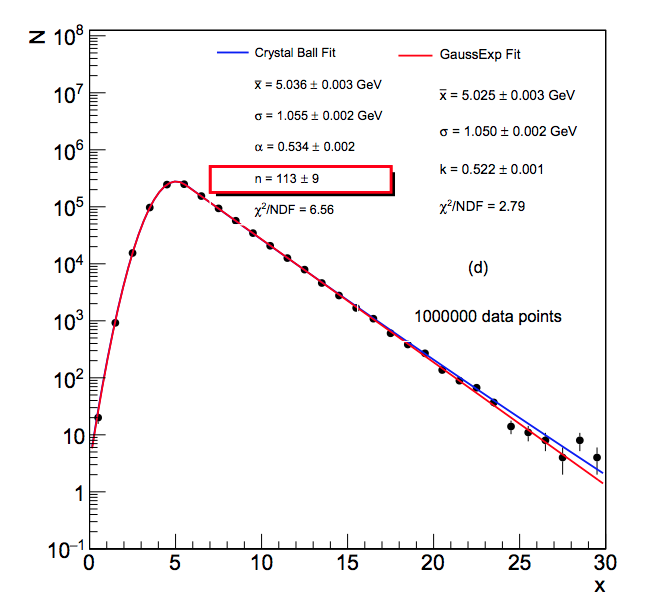
\includegraphics[width=\textwidth]{Figures/crystalball.png}
\caption{Comparison of fits to data using the Crystal Ball function and the Gaussian-Exponential. Figure taken from \cite{alternatecrystalball}.}
\label{fig:crystalball}
\end{figure}

\subsection{Numerical De-Smearing with libNEST}\label{sec:desmearprelim}
Either of the equations shown in \ref{eq:crystalball} and \ref{eq:gausexp} would make the calculation of the smearing corrections extremely cumbersome. Additionally, if there is additional correlation between $\sigma_{e,det}$, $\sigma_{\gamma,det}$, and $\sigma_{R}$ that we have not accounted for the correction factors we calculate would be wrong. For these reasons, we elect to instead calculate the smearing corrections for $E_{rec}$, $N_{\gamma}$, and $N_{e}$ numerically. In the libNEST code, we have a well-developed and well-tested model of the LUX detector resolution that is perfectly suited to this purpose. The libNEST code also models the energy threshold, which will also have an effect on the observed spectral shape but was not included in our calculations up to this point. With the addition of the model of the S2 tails developed in section \ref{sec:s2tails}, we will also be able to characterize and quantize the systematic effects that they introduce to our yields and recombination measurements.

We will begin by defining a set of energy bins to go along with the electric field bins we defined in section \ref{sec:fieldbins}. Then we will use the existing libNEST yields and recombination model to extract a set of corrections for energy, $N_e$, and $N_{\gamma}$:
\begin{align}
\label{eq:nestEcorr}C_{E,ij}&=\frac{\langle E_{input} \rangle_{ij}}{\langle E_{rec,NEST} \rangle_{ij}} \\[1em]
\label{eq:nestS1corr}C_{\gamma,ij}&=\frac{LY_{NEST}(\langle E_{true} \rangle_{ij},\langle \mathcal{E} \rangle_j)\cdot \langle E_{input} \rangle_{ij}}{\langle n_{\gamma,NEST} \rangle_{ij}} \\[1em]
\label{eq:nestS2corr}C_{e,ij}&=\frac{QY_{NEST}(\langle E_{true} \rangle_{ij},\langle \mathcal{E} \rangle_j)\cdot \langle E_{input} \rangle_{ij}}{\langle n_{e,NEST} \rangle_{ij}} 
\end{align}
Here, $\langle \rangle_{ij}$ indicates an averaged value over events selected by both the $i^{th}$ reconstructed energy bin and $j^{th}$ electric field bin, as defined in section \ref{sec:fieldbins}. $E_{input}$ is the input energy of the events, and $n_{\gamma,NEST}=S1_{NEST}/G1$ and $n_{e,NEST}=S2_{NEST}/G2$ are the output charge and light signals after the yields, recombination, detector efficiency, and detector resolution have all been simulated. $G1$ and $G2$ are the overall light and charge efficiencies used in the libNEST model and will be set to be equal to those measured in the data. $LY_{NEST}$ and $QY_{NEST}$ are the input light and charge yields for events with an energy equal to $\langle E_{input} \rangle_{ij}$. In the existing libNEST model there is no explicit value defined for $LY_{NEST}(E,\mathcal{E})$ and $QY_{NEST}(E,\mathcal{E})$, but rather a combination of other parameters come together to reproduce $LY$ and $QY$ as a function of electric field and energy. For this reason, we will approximate $LY_{NEST}(\langle E_{input} \rangle_{ij},\langle \mathcal{E} \rangle_j)$ and $QY_{NEST}(\langle E_{input} \rangle_{ij},\langle \mathcal{E} \rangle_j)$ by generating a flat spectrum in libNEST, and measuring: 
\begin{equation}\label{eq:flatlyqy}
\begin{split}
LY_{NEST}(\langle E_{input} \rangle_{ij},\langle \mathcal{E} \rangle_j) &\approx \langle N_{\gamma,NEST} \rangle_{ij}/\langle E_{input} \rangle_{ij}\\ 
QY_{NEST}(\langle E_{input} \rangle_{ij},\langle \mathcal{E} \rangle_j) &\approx \langle N_{e,NEST} \rangle_{ij}/\langle E_{input} \rangle_{ij},
\end{split}
\end{equation}
where $N_{\gamma,NEST}$ and $N_{e,NEST}$ are the true number of photons and electrons simulated in the event, before detector resolution is applied, but after the recombination is simulated. The modified version of libNEST which will be used to calculate the corrections for the final measurements will use explicit functions for $LY_{NEST}(E,\mathcal{E})$ and $QY_{NEST}(E,\mathcal{E})$, so the approximation shown in equation \ref{eq:flatlyqy} will not be necessary.

We will apply these corrections to the average S1 and S2 signal measured in each reconstructed energy bin in order to produce the measured, un-smeared averages $\langle E_{true} \rangle_{ij}$, $\langle n_{e} \rangle_{ij}$, and $\langle N_{\gamma} \rangle_{ij}$:
\begin{align}
\label{eq:datEtrue}\langle E_{true} \rangle_{ij}&=C_{E,ij} \cdot \left\langle E_{rec} \right\rangle_{ij} \\[1em]
\label{eq:datNytrue}\langle N_{\gamma} \rangle_{ij}&=C_{\gamma,ij} \cdot \left\langle n_{\gamma}\right\rangle_{ij} \\[1em]
\label{eq:datNetrue}\langle N_{e} \rangle_{ij}&= C_{e,ij} \cdot \left\langle n_e\right\rangle_{ij}
\end{align}
where we have taken $W=\frac{1}{73.0 \ \pm 1.1}$ keV per quanta. 
\begin{figure}[h!]
\centering
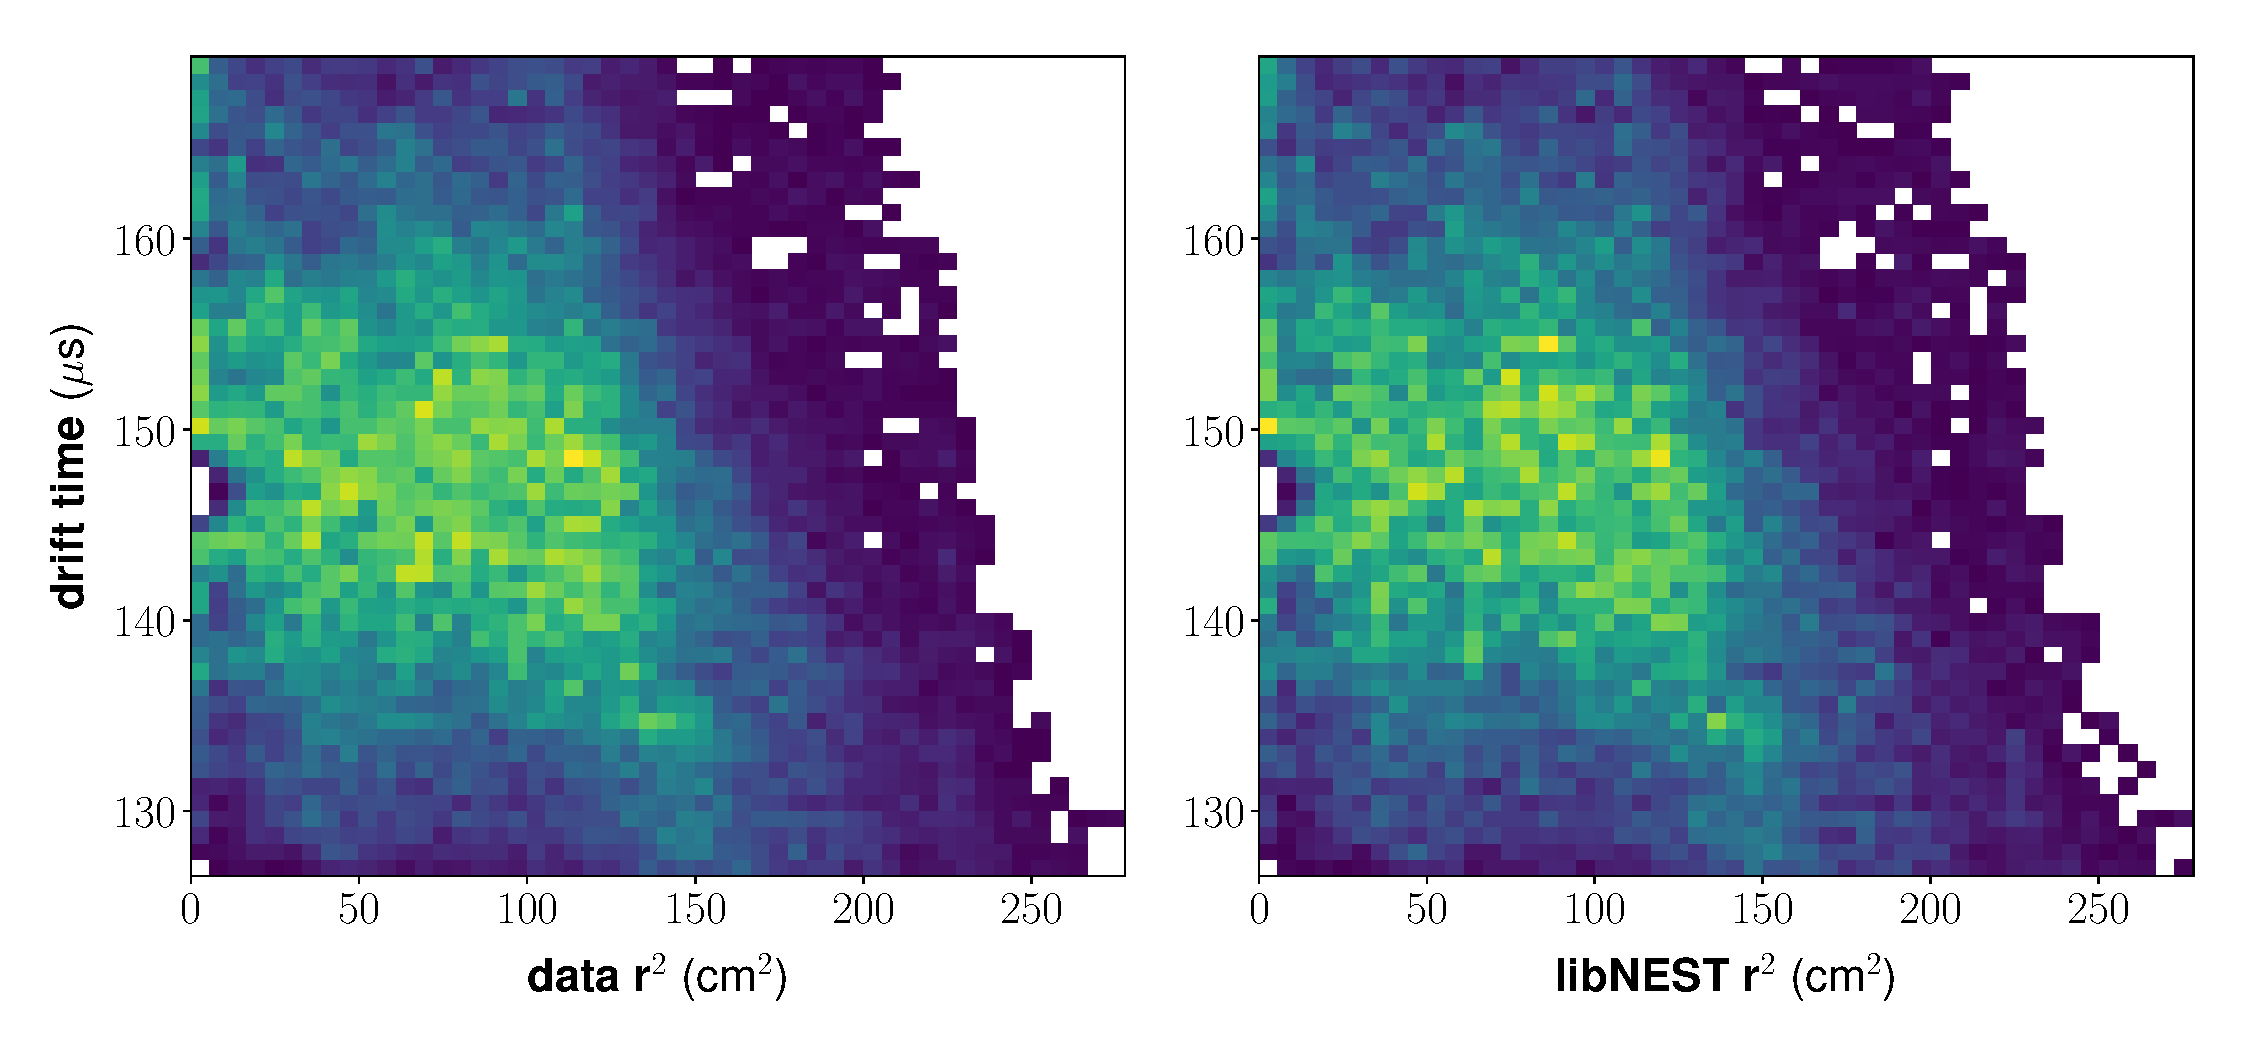
\includegraphics[width=\textwidth]{Figures/yields_corrections/C14_eFcut_gfdcm_180Vcm_prelim.pdf}
\caption{Selected carbon-14 events in the 180 V/cm electric field bin. Events from data are shown on the left, and libNEST simulated events are on the right. }
\label{fig:efcut_180vcm}
\end{figure}


\subsection{Preliminary Measurement of QY}\label{sec:qyprelim}
As an example, we will examine the measured corrections for the 180 V/cm field bin, using the ``gfdcm'' corrected data. A 2D-histogram of the radius-squared and drift time of the selected events for both data and libNEST simulation is shown in figure \ref{fig:efcut_180vcm}. The x-position, y-position, efficiency-correction factors, drift time, and electric field of the simulated events are all randomly drawn from the population of data events, so the two histograms in figure \ref{fig:efcut_180vcm} are identical, except for random fluctuations. 
\begin{figure}[h!]
\centering
\begin{subfigure}{0.5\textwidth}
  \centering
  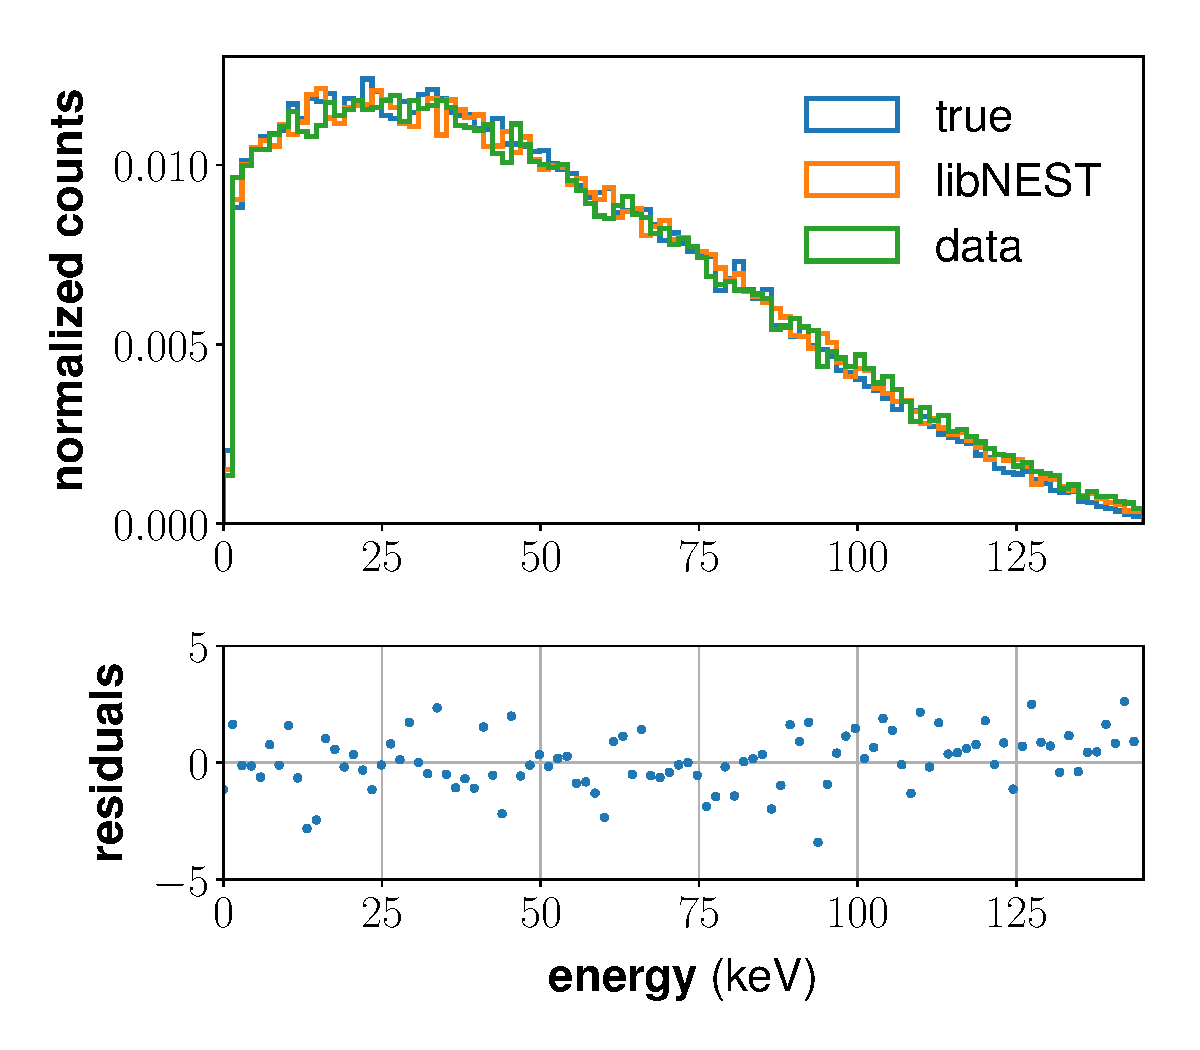
\includegraphics[width=\textwidth]{Figures/yields_corrections/C14_spectrum_gfdcm_180Vcm_prelim.pdf}
  \caption{}
  \label{fig:c14spec_180_prelim}
\end{subfigure}%
\begin{subfigure}{0.5\textwidth}
  \centering
  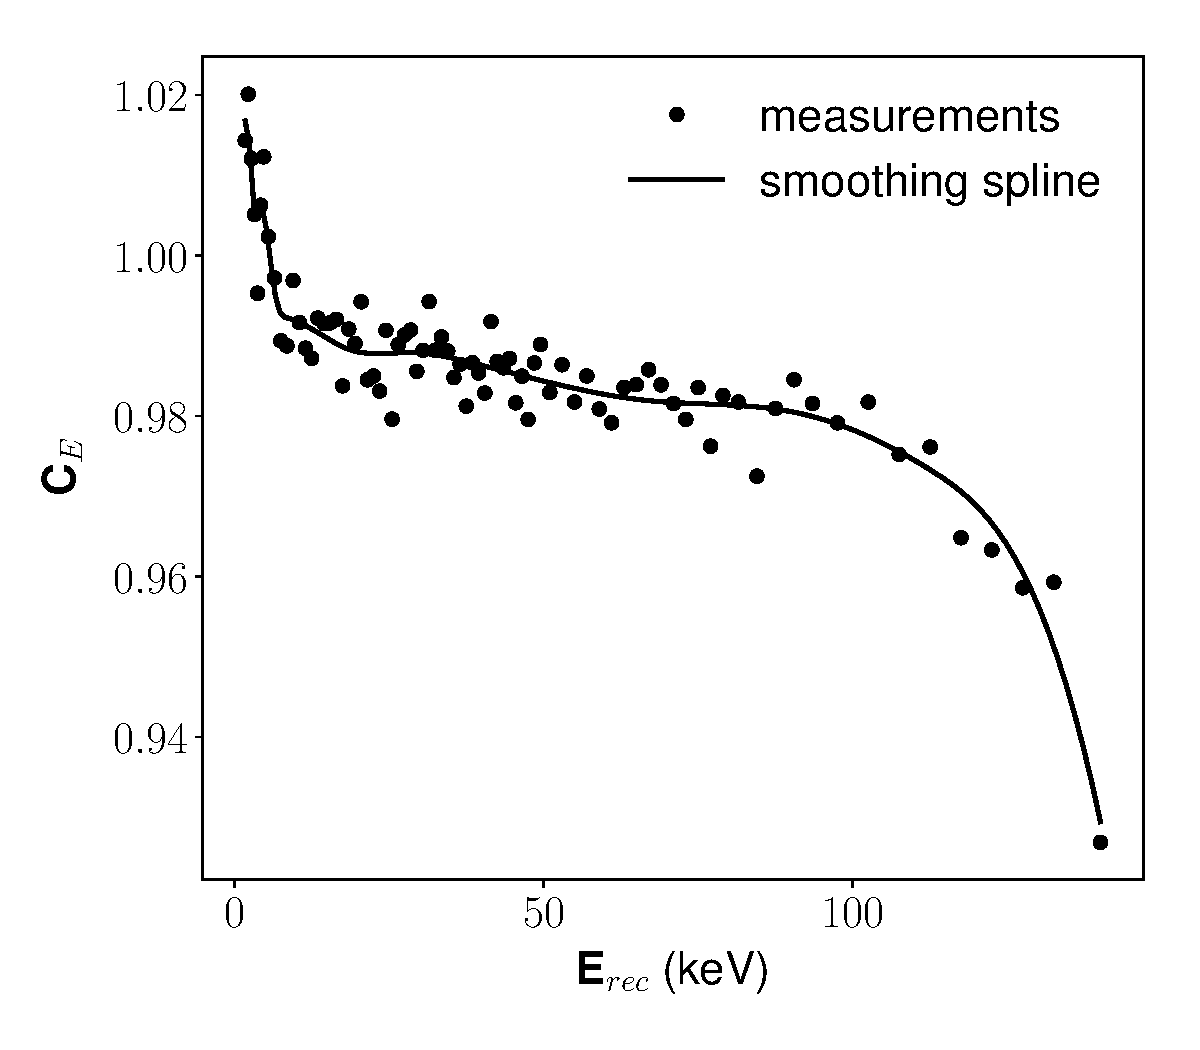
\includegraphics[width=\textwidth]{Figures/yields_corrections/C14_E_correction_gfdcm_180Vcm_prelim.pdf}
  \caption{}
  \label{fig:c14ecorr_180_prelim}
\end{subfigure}
\caption{Carbon-14 spectrum (left) and the calculated energy smearing correction (right). The residuals show a comparison of the data spectrum with the libNEST simulated spectrum. There is decent agreement over the entire energy range, with the reduced chi-squared coming out to 1.4. The square markers in the right-hand plot show the calculated values of the correction factor, and the continuous black line shows the smoothing spline.}
\label{fig:c14_ecorr}
\end{figure} 
We define our reconstructed energy bins such that there is an approximately constant number of events in each bin. From 1.5 to 5 keVee, we bin in steps of 0.5 keVee. We allow this region to have fewer counts in order to minimize the spread in energies within the bin. From there we incrementally increase the bin width to account for the falling $\frac{dN}{dE}$. The bin widths and their associated energy regions  are shown in table \ref{tab:ebins}.
\begin{table}[h!]
\centering
    \begin{tabular}{ c || c | c | c | c | c | c  }
    \hline
    Energy Range (keV) & 1.5-5.0 & 5-50  & 50-80 & 80-95 & 95-135 & 135-145\\
    \hline
    Bin Width (keV)         &  0.5       & 1      & 2        & 3         & 5           & 10 \\
    \hline
    \end{tabular}
    \caption{Reconstructed energy bin widths and their associated energy ranges}
    \label{tab:ebins}
\end{table}

We first examine the measured carbon-14 energy spectrum and how it compares to the simulated spectrum which is shown in figure \ref{fig:c14spec_180_prelim}. There is decent agreement between simulation and data; other than a possible small upward slope above 100 keV, there is no clear systematic trend in the residuals, and the reduced chi-squared is 1.4.

We calculate the energy smearing correction for each reconstructed energy bin as described in equations \ref{eq:nestEcorr} and \ref{eq:flatlyqy}. Using the SciPy.interpolate ``UnivariateSpline'' tool with the smoothing factor set to 0.0005 \cite{scipy}, we smooth our newly measured set of $C_{E,i,180}$. We make adjustments to the smoothing factor as needed to make the spline well-conditioned and to make sure it picks up the first and last points.
\begin{figure}[h!]
\centering
\begin{subfigure}{0.5\textwidth}
  \centering
  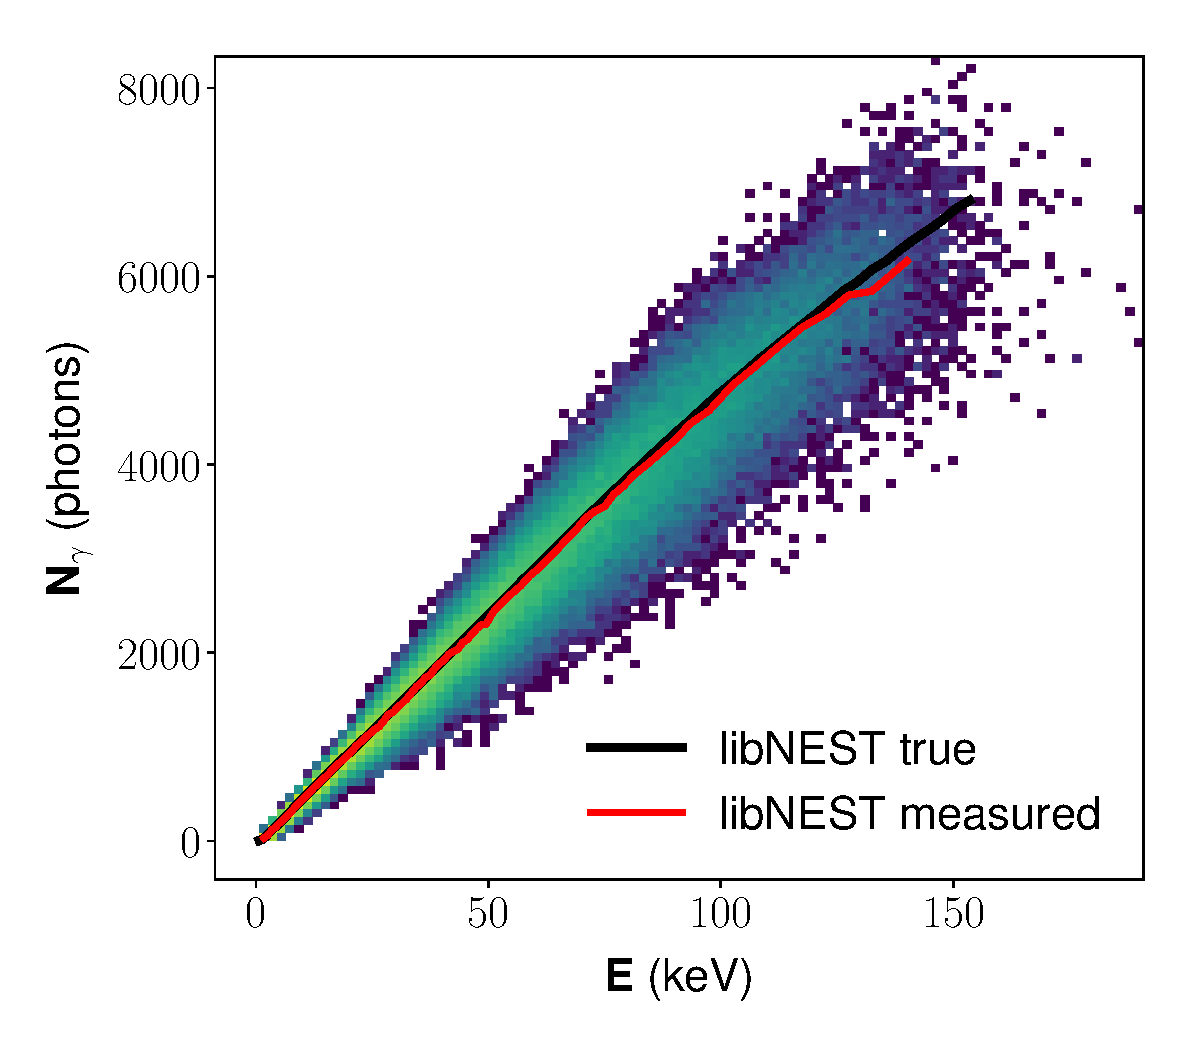
\includegraphics[width=\textwidth]{Figures/yields_corrections/C14_LN_heatmap_gfdcm_180Vcm_prelim.pdf}
  \caption{}
\end{subfigure}%
\begin{subfigure}{0.5\textwidth}
  \centering
  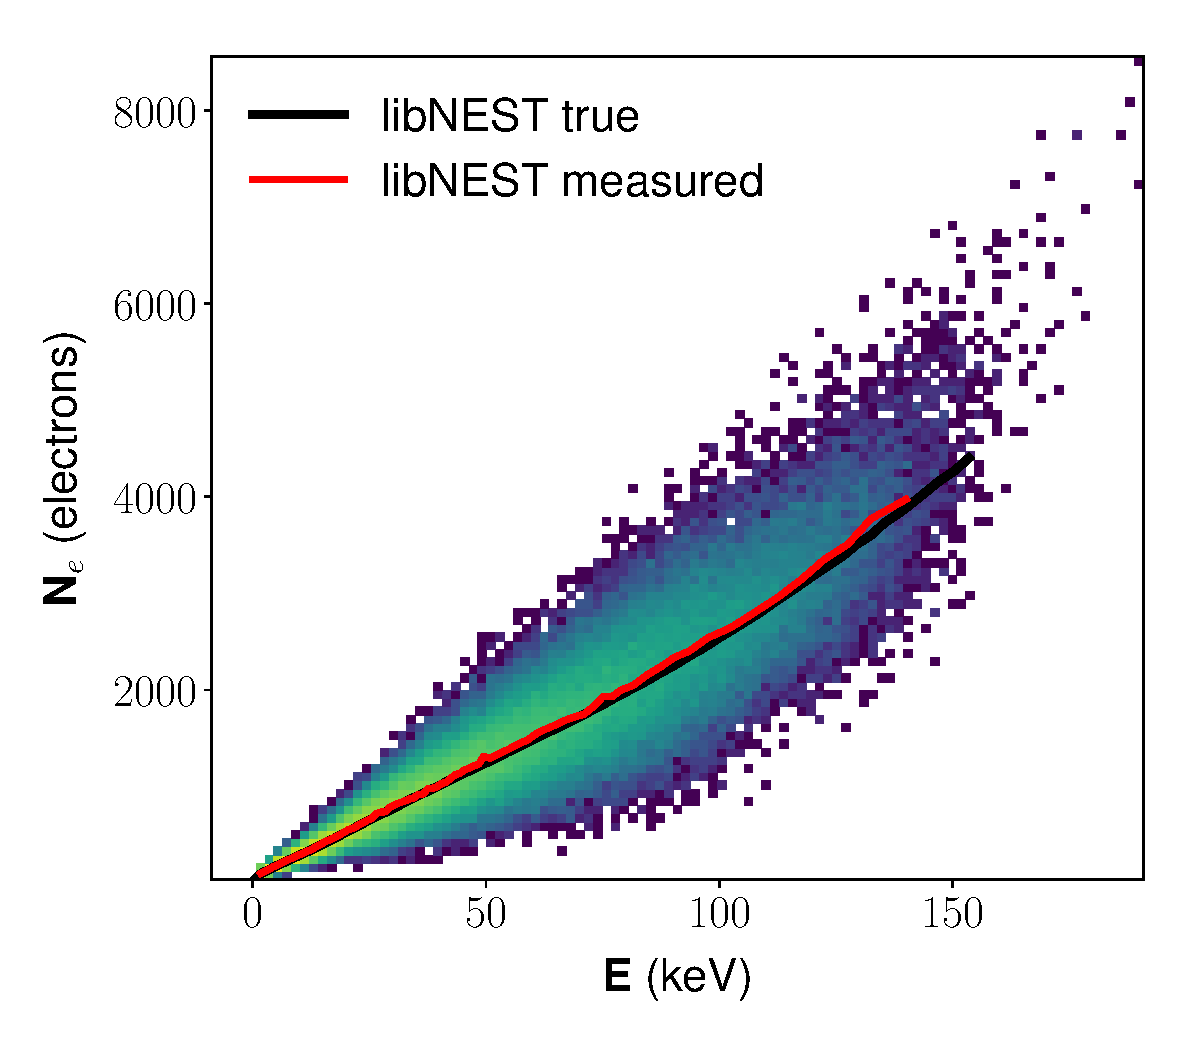
\includegraphics[width=\textwidth]{Figures/yields_corrections/C14_QN_heatmap_gfdcm_180Vcm_prelim.pdf}
  \caption{}
\end{subfigure}
\caption{The red lines show the measurements of  $\langle S1_{NEST}/G1 \rangle_{i,180}$ (a) and $\langle S2_{NEST}/G2 \rangle_{i,180}$ (b) for the preliminary carbon-14 model. The black lines show $\langle N_{\gamma} \rangle_{i,180}$ (a) and $\langle N_{e} \rangle_{i,180}$} (b).
\label{fig:lnqn_180_prelim}
\end{figure} 

The next step is to measure the smearing corrections for S1 and S2. Figure \ref{fig:lnqn_180_prelim} (a) and (b) show the simulated bands of $n_{\gamma,NEST}=S1_{NEST}/G1$ and $n_{e,NEST}=S2_{NEST}/G2$ versus reconstructed energy. We first aim to measure the peak value of $n_{\gamma,NEST}$ in our set of reconstructed energy bins. In each of these bins, we take the arithmetic mean ($\overline{n}_{\gamma,NEST}$) and standard deviation (std$(n_{\gamma,NEST})$) of the $n_{\gamma,NEST}$ population. To reject the events which are most severely affected by the pathological tails, a further cut is made:
\begin{equation}
\overline{n}_{\gamma,NEST}-\text{std}(n_{\gamma,NEST})<n_{\gamma,NEST}<\overline{n}_{\gamma,NEST}+2\cdot \text{std}(n_{\gamma,NEST})
\end{equation}
We then fit a Gaussian to the population of $n_{\gamma,NEST}$ which pass this cut. The peak value of this Gaussian in the $i^{th}$ bin is taken to be $\langle n_{\gamma,NEST} \rangle_{i,180}$. We follow a similar procedure to find $\langle n_{e,NEST} \rangle_{i,180}$, but the selection cut is instead:
\begin{equation}
\overline{n}_{e,NEST}-2\cdot \text{std}(n_{e,NEST})<n_{e,NEST}<\overline{n}_{e,NEST}+ \text{std}(n_{e,NEST})
\end{equation}
With $\langle n_{\gamma,NEST} \rangle_{i,180}$ and $\langle n_{e,NEST} \rangle_{i,180}$ in hand, we now calculate $C_{\gamma}$ and $C_e$ using equations \ref{eq:nestS1corr} and \ref{eq:nestS2corr}.
\begin{figure}[h!]
\centering
\begin{subfigure}{0.5\textwidth}
  \centering
  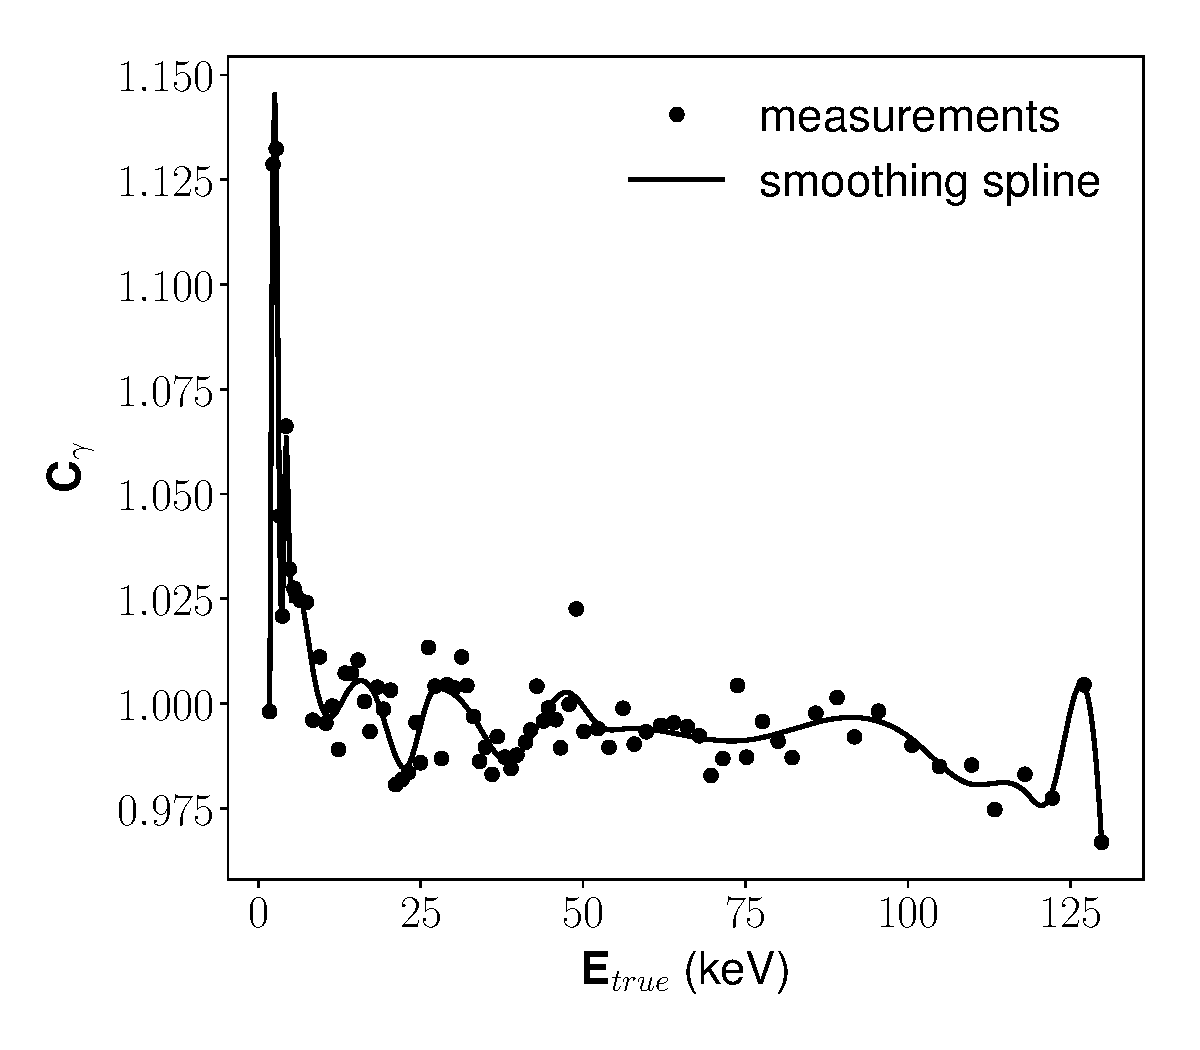
\includegraphics[width=\textwidth]{Figures/yields_corrections/C14_LN_correction_gfdcm_180Vcm_prelim.pdf}
  \caption{}
\end{subfigure}%
\begin{subfigure}{0.5\textwidth}
  \centering
  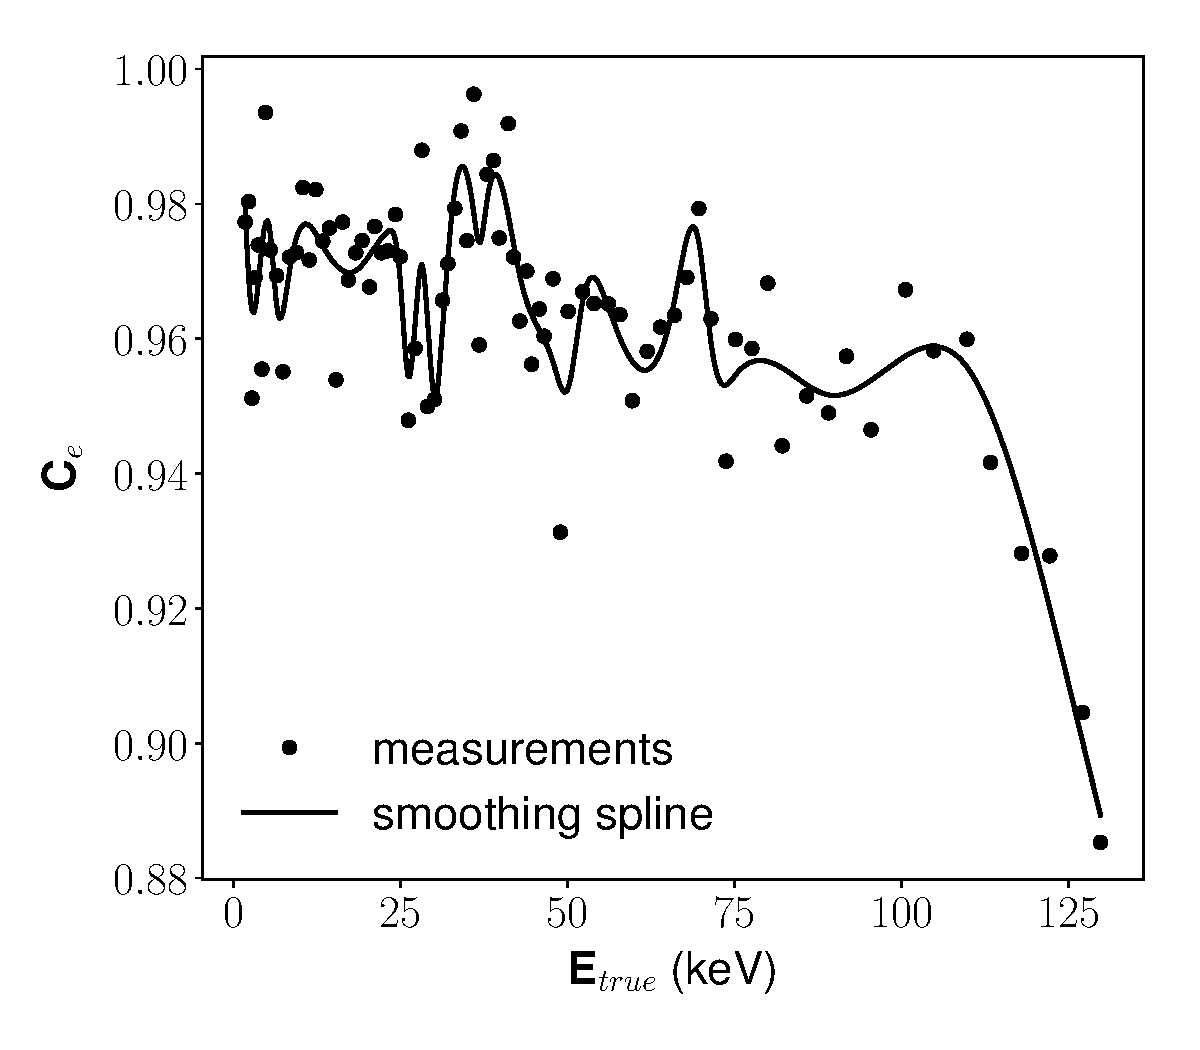
\includegraphics[width=\textwidth]{Figures/yields_corrections/C14_QN_correction_gfdcm_180Vcm_prelim.pdf}
  %\label{fig:intlin}
\end{subfigure}
\caption{This figure shows the smearing correction for S1 (a) and S2 (b). The square markers show the calculated values of the correction factors, and the continuous black lines show the smoothing spline.}
\label{fig:lnqn_correction}
\end{figure}

We calculate $\left\langle n_{\gamma} \right\rangle_{i,180}$ and $\left\langle n_e \right\rangle_{i,180}$ using the same method we used to calculate $\langle n_{\gamma,NEST} \rangle_{i,180}$ and $\langle n_{e,NEST} \rangle_{i,180}$. Finally, we can now obtain $\langle N_{\gamma} \rangle_{i,180}$ and $\langle N_{e} \rangle_{i,180}$ using equations \ref{eq:datNytrue} and \ref{eq:datNetrue}, respectively. It is then simple to calculate the charge and light yield that we will use in our updated libNEST model:
\begin{align}
LY_{i,180}=\frac{\langle N_{\gamma} \rangle_{i,180}}{\langle E_{true} \rangle_{i,180}}\\[1em]
QY_{i,180}=\frac{\langle N_{e} \rangle_{i,180}}{\langle E_{true} \rangle_{i,180}}
\end{align}
\begin{figure}[h!]
\centering
\begin{subfigure}{0.5\textwidth}
  \centering
  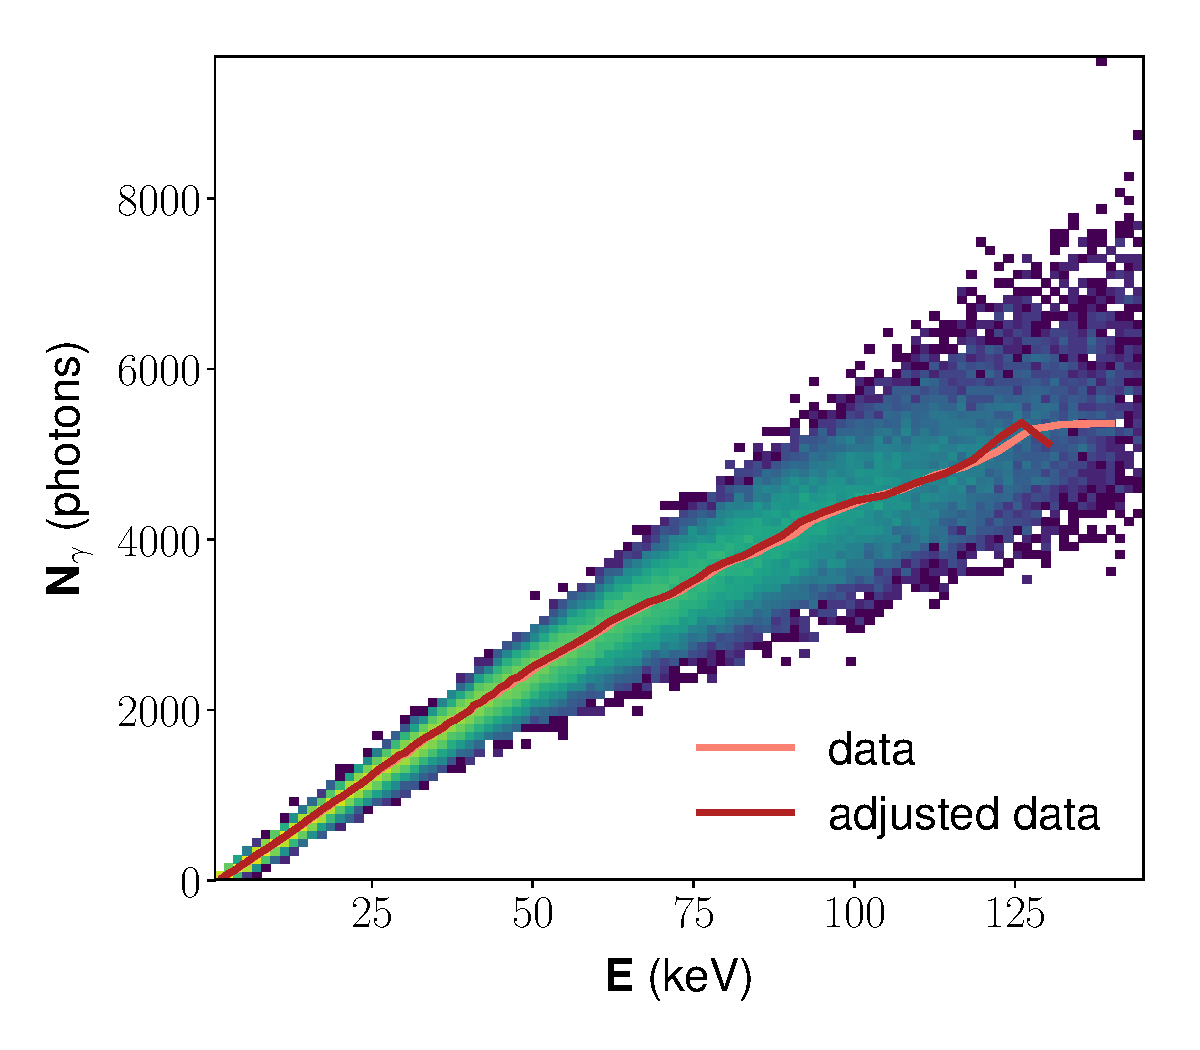
\includegraphics[width=\textwidth]{Figures/yields_corrections/C14_LN_heatmap_dat_gfdcm_180Vcm_prelim.pdf}
  \caption{}
\end{subfigure}%
\begin{subfigure}{0.5\textwidth}
  \centering
  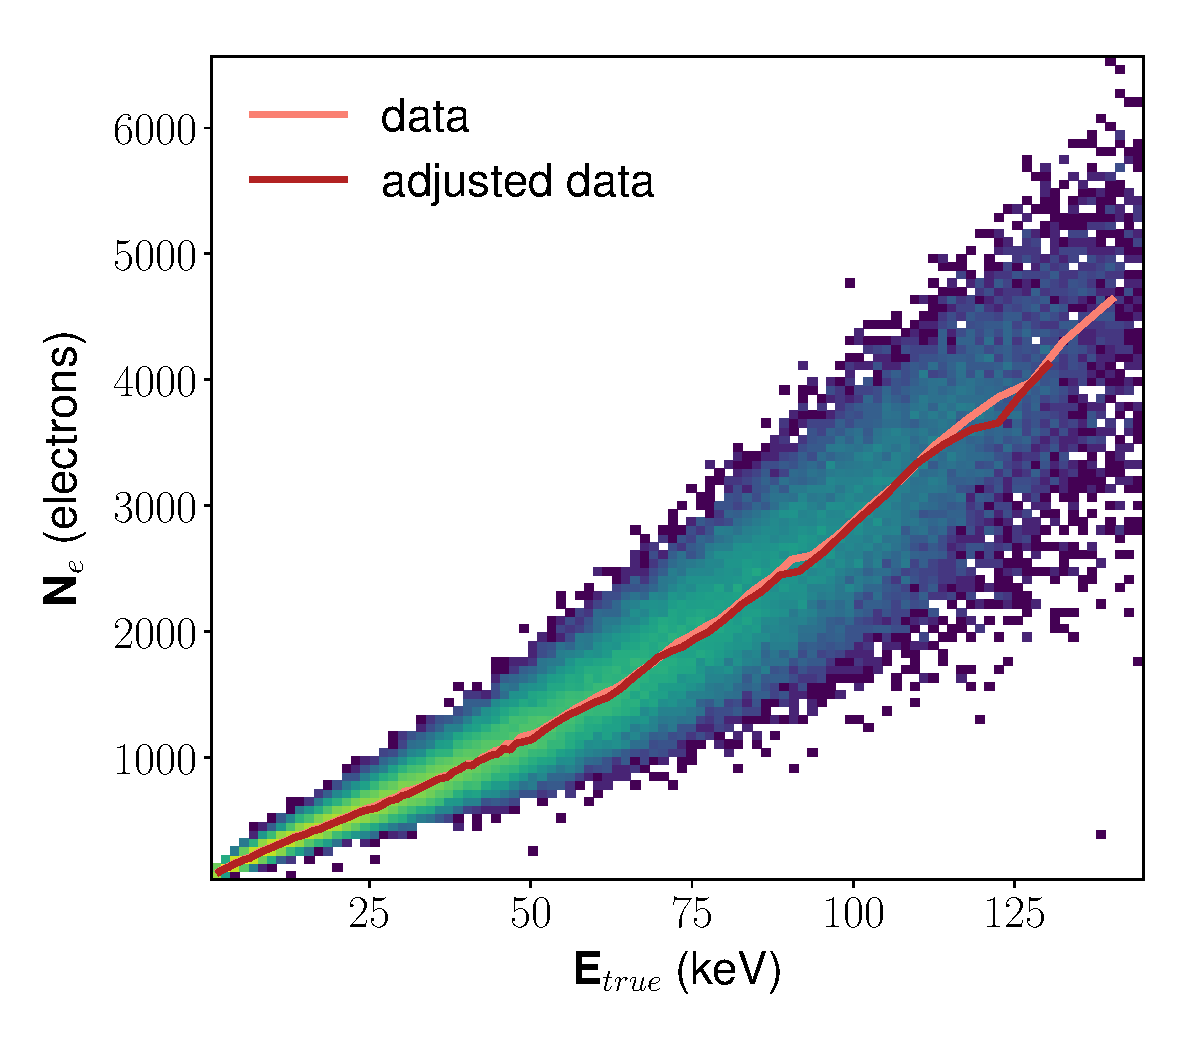
\includegraphics[width=\textwidth]{Figures/yields_corrections/C14_QN_heatmap_dat_gfdcm_180Vcm_prelim.pdf}
  \caption{}
\end{subfigure}
\begin{subfigure}{0.5\textwidth}
  \centering
  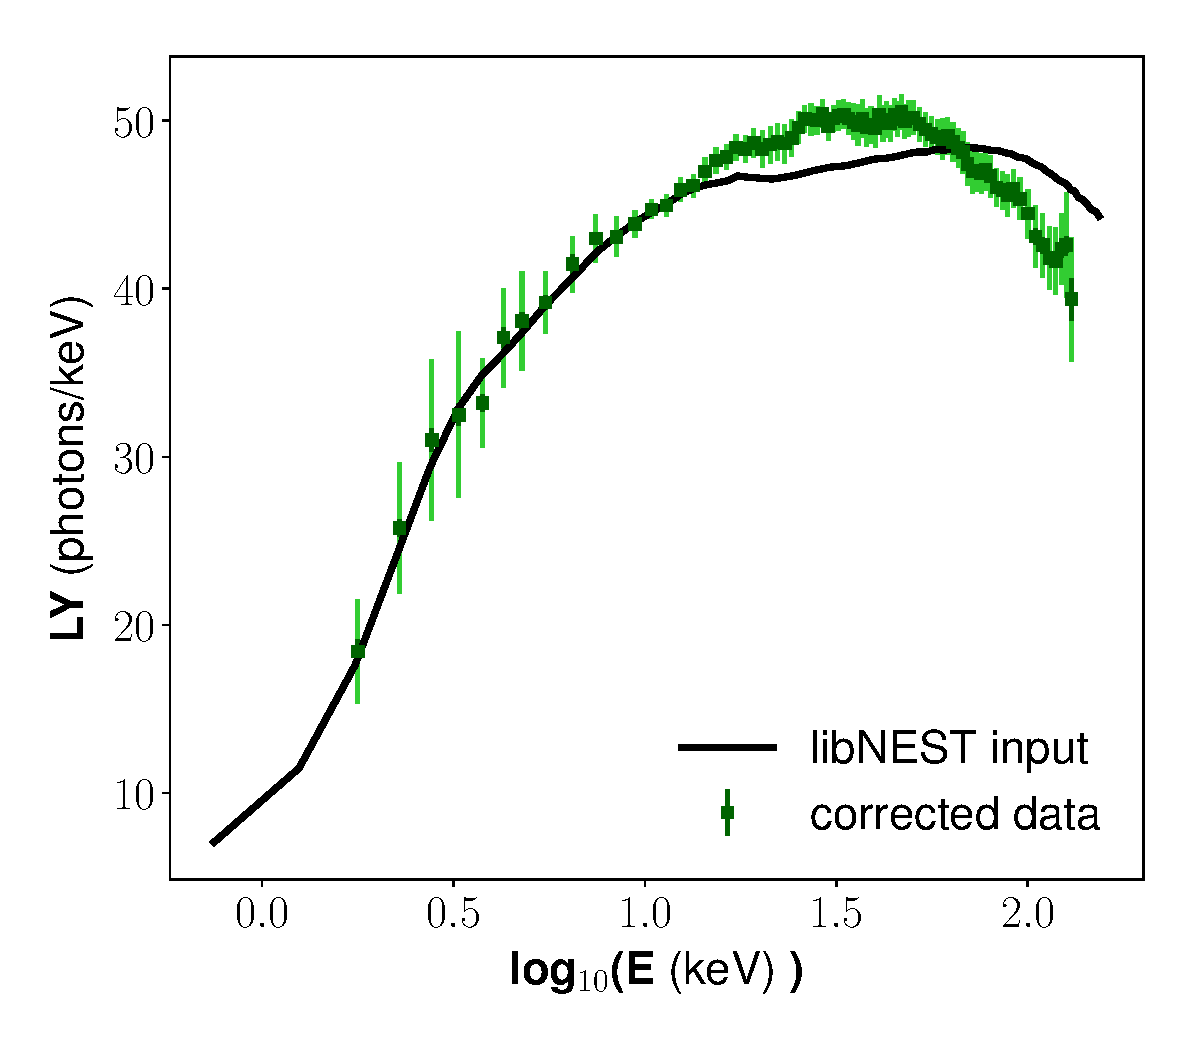
\includegraphics[width=\textwidth]{Figures/yields_corrections/C14_LY_final_gfdcm_180Vcm_prelim.pdf}
  \caption{}
\end{subfigure}%
\begin{subfigure}{0.5\textwidth}
  \centering
  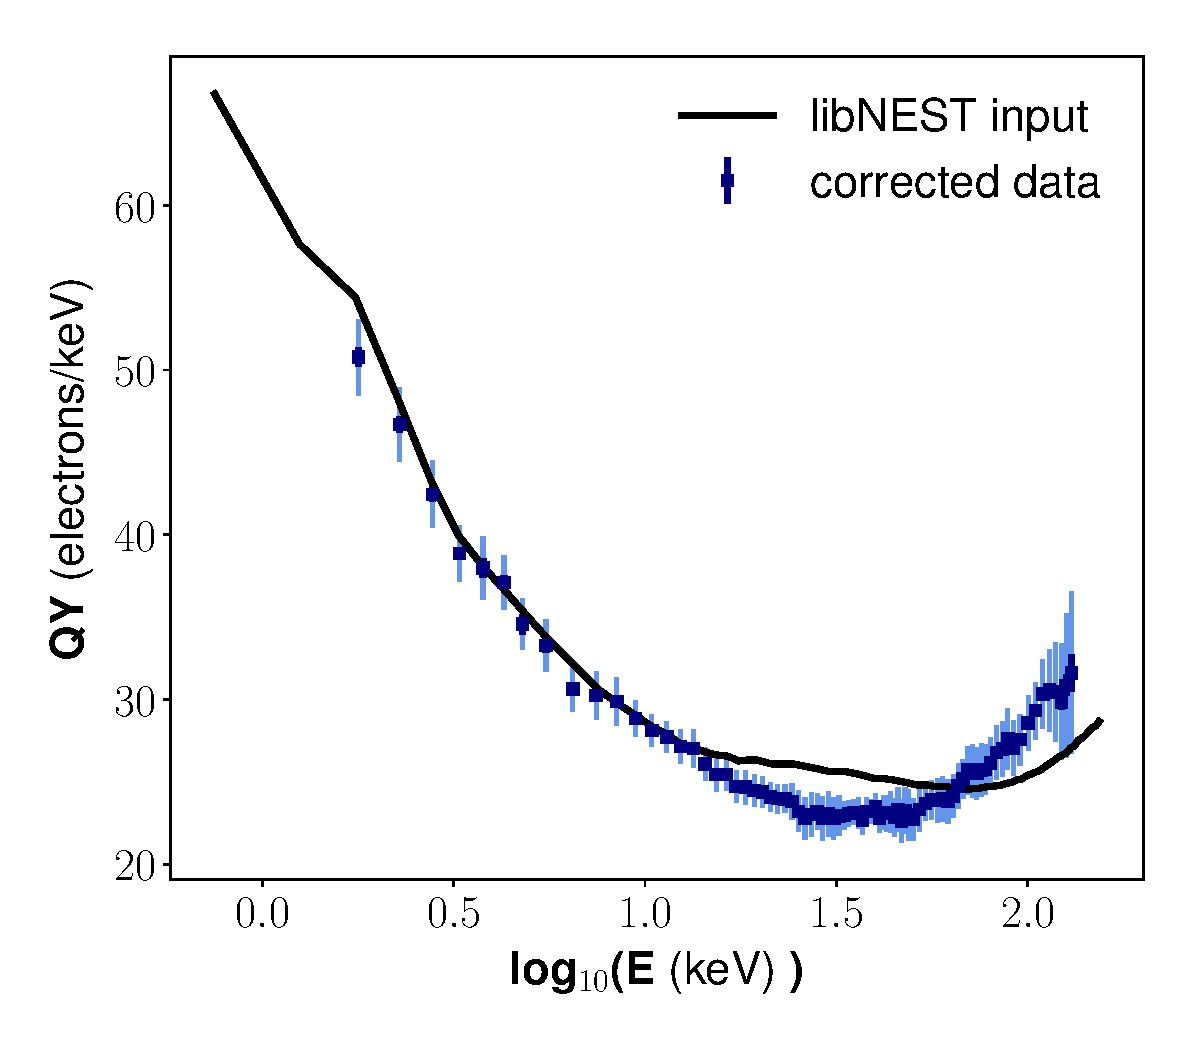
\includegraphics[width=\textwidth]{Figures/yields_corrections/C14_QY_final_gfdcm_180Vcm_prelim.pdf}
  \caption{}
\end{subfigure}
\caption{Preliminary measurements of $\langle N_{\gamma} \rangle_{i,180}$ (a) and $\langle N_{e} \rangle_{i,180}$ (b), along with the associated calculations of $LY$ (c) and $QY$ (d). In the top plots, (a) and (b), the heat-maps shows the measured, unadjusted populations of $n_{\gamma}=S1c/G1$ and $n_{e}=S2c/G2$. The light red lines show the unadjusted peak values versus unadjusted energy. The dark red lines show these trends after the smearing corrections are applied. The lower plots show the fully adjusted measurements of $LY= \langle N_{\gamma} \rangle_{i,180}/\langle E_{true} \rangle_{i,180}$, and $QY= \langle N_{e} \rangle_{i,180}/\langle E_{true} \rangle_{i,180}$. The light colored error-bars show the systematic+statistical uncertainty, while the darker error-bars show the statistical uncertainty alone. The black lines show the existing NEST values of $LY$ and $QY$.  }
\label{fig:dat_lnqn_heatmap}
\end{figure}

Figure \ref{fig:dat_lnqn_heatmap} shows the results of our yields measurements. In these results, we have taken the size of the smearing correction to be our systematic error ($\sigma_{syst}=|1-C|$). In defining these errors, we want to account for statistical fluctuations in the correction factor and one that is steeply sloped. If, for example, $|1-C_{e,i}|$ is much greater than $|1-C_{e,i-1}|$, then $|1-C_{e,i}|$ is likely a better estimate of $\sigma_{e,syst,i}$ than $|1-C_{e,i-1}|$. For this reason, we define $\sigma_{syst,i}=\text{max}(|1-C_{i-1}|,|1-C_i|,|1-C_{i+1}|)$.

The fitting error is taken as the statistical error and is shown as dark green error-bars in (c), and dark blue error-bars in (d). The light-colored error-bars in (c) and (d) show the systematic plus statistical uncertainties. Below about 15 keV there is good agreement between the existing NEST model (shown as the black lines in (c) and (d)) and the measurements. In this region, $LY$ and $QY$ was tuned by the measurements using LUX Run03 tritium, so good agreement is expected. Above this value, there are no measurements of beta-decay yields, and the discrepancy between data and NEST is large.


\begin{figure}[h!]
\centering
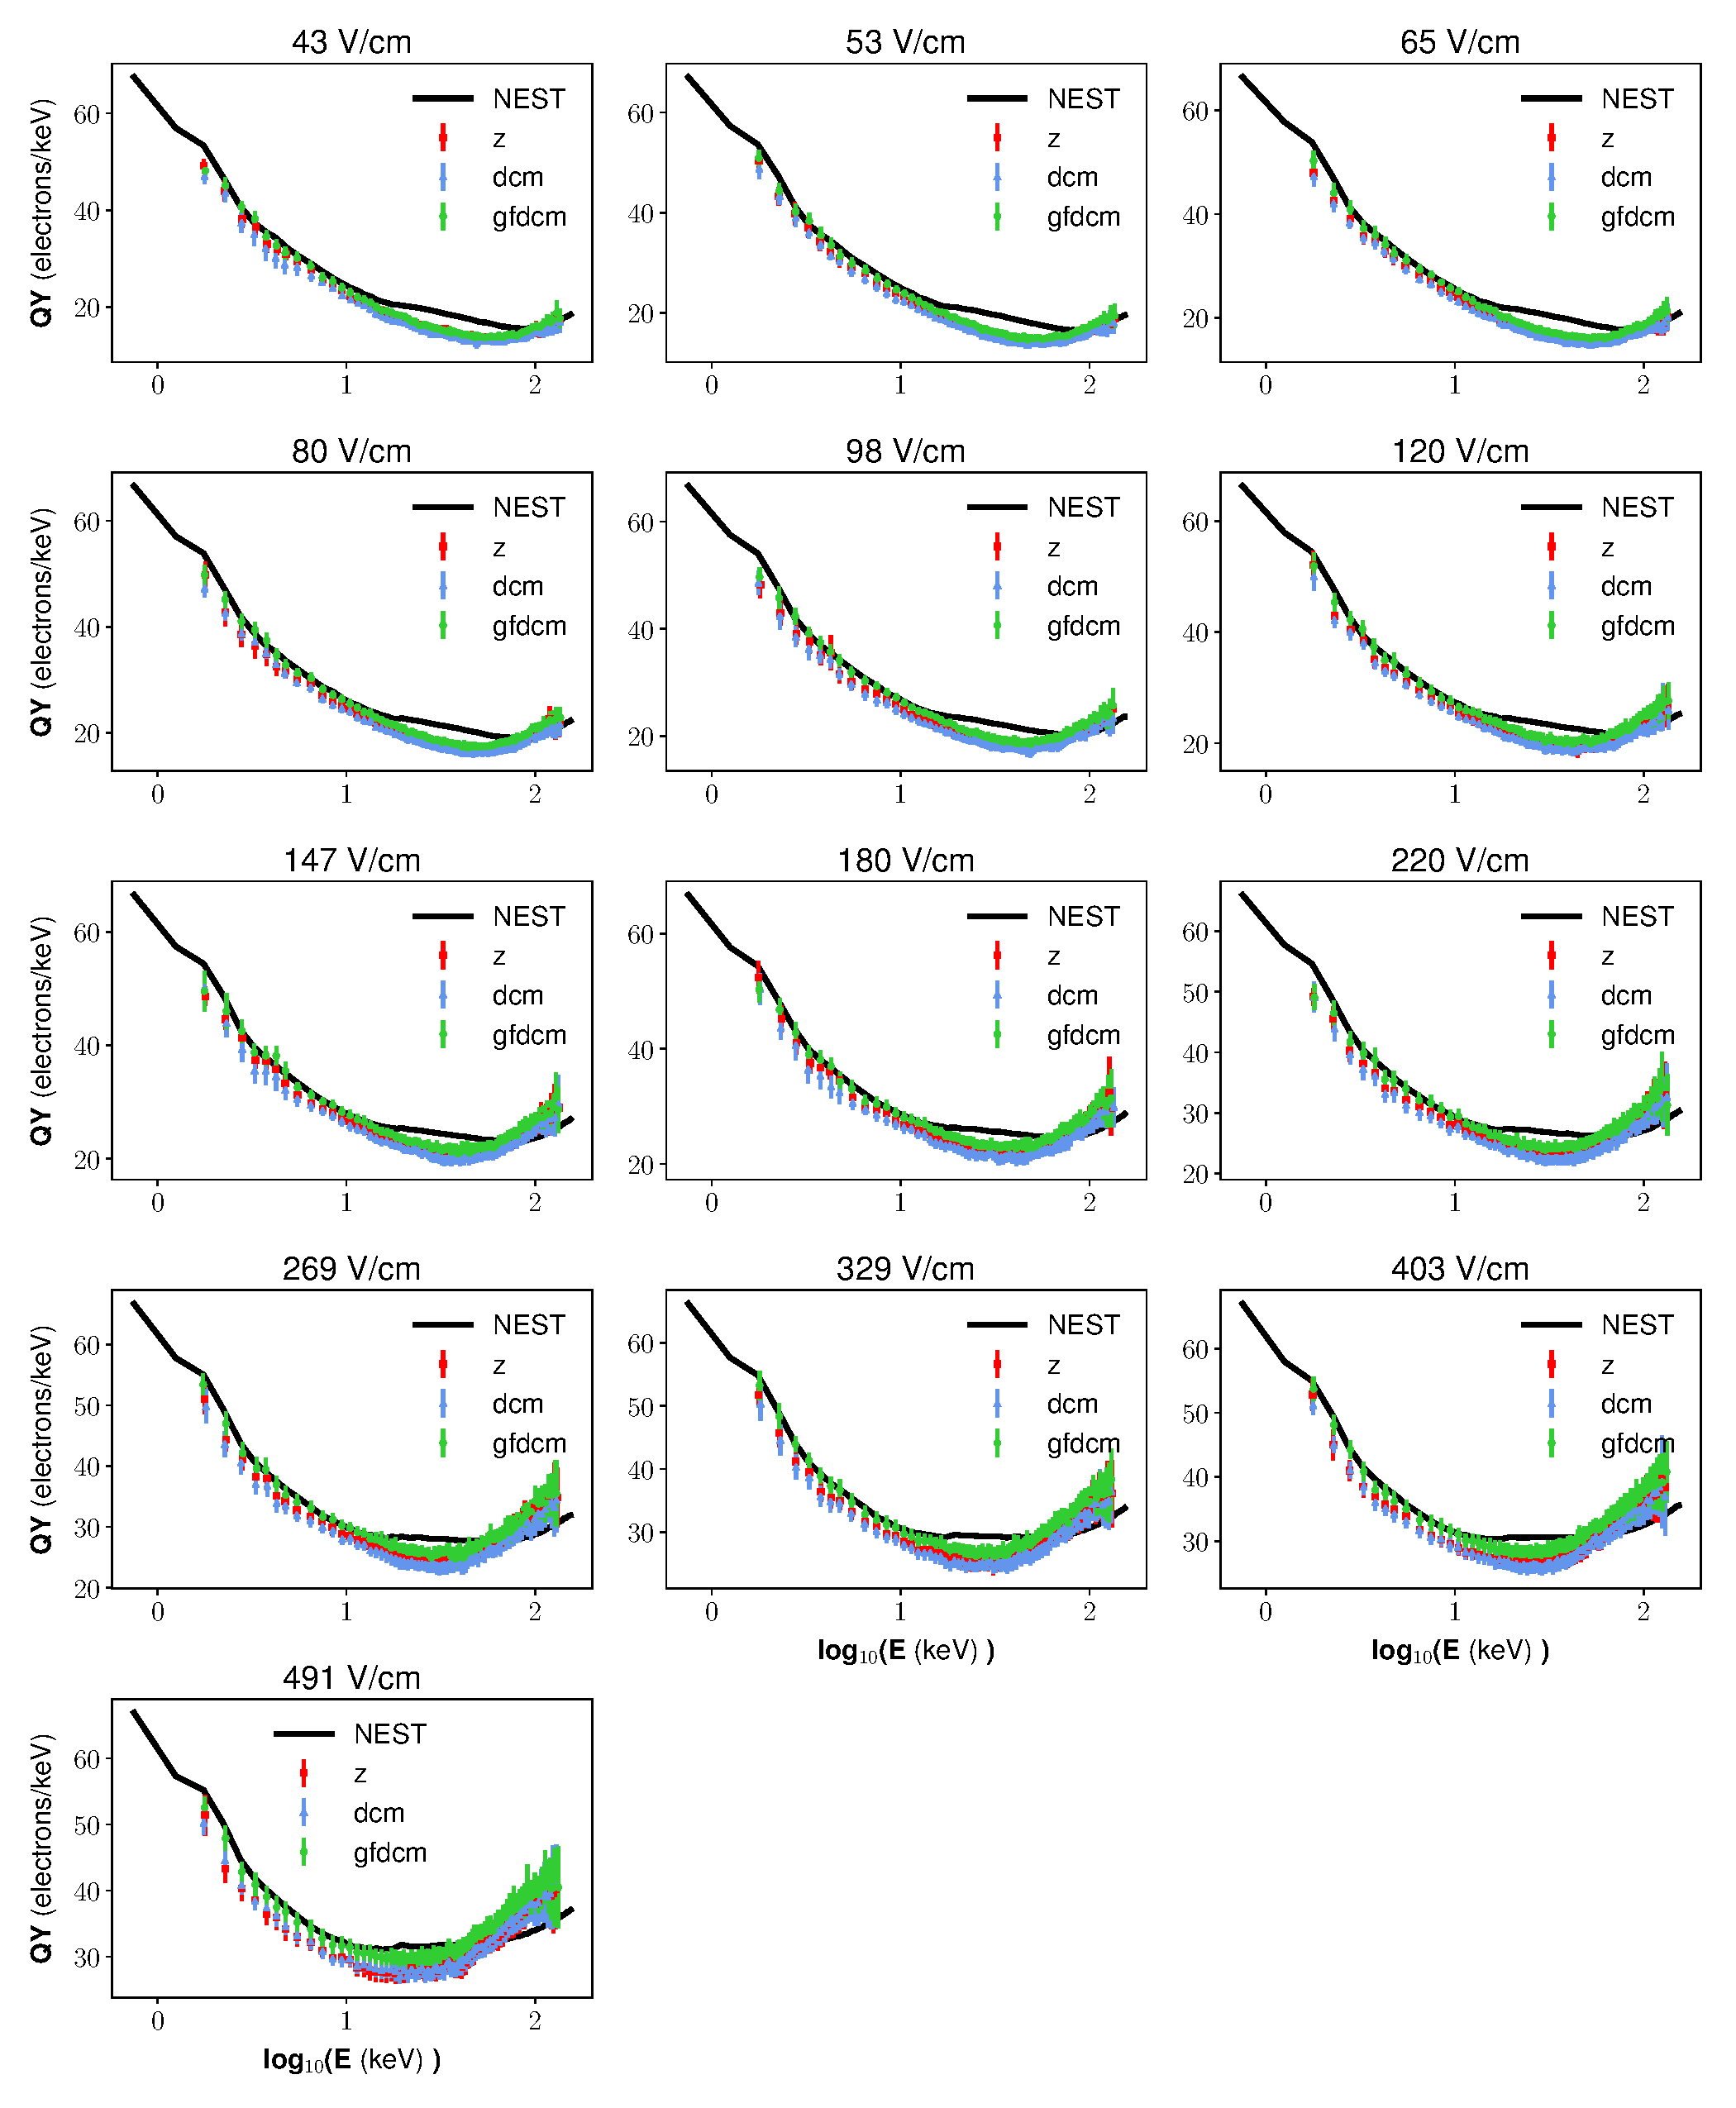
\includegraphics[width=\textwidth]{Figures/C14_QY_prelim.pdf}
\caption{Preliminary carbon-14 charge yield for the three efficiency corrections being studied, in each of the 13 electric field bins defined in \ref{sec:fieldbins}. The x-axis here represents the true event energy, obtained by applying the smearing corrections. The charge yields measured here will be used to fine-tune the NEST model in order to obtain a more accurate set of corrections.}
\label{fig:C14_QY_prelim}
\end{figure}
In the combined energy model, we assume that $LY+QY=1/W$, where $1/W=73 \ \pm1.1$ quanta per keV. It is not necessary to define both $LY$ and $QY$ when generating a simulated event; we can instead define only $QY$ and allow $LY=73-QY$. It would also be possible to define $LY$ and let $QY=73-LY$, but measurements of $LY$ tend to have larger uncertainties because the $S1$ signal has a smaller gain than the $S2$ signal. 

\begin{figure}[h!]
\centering
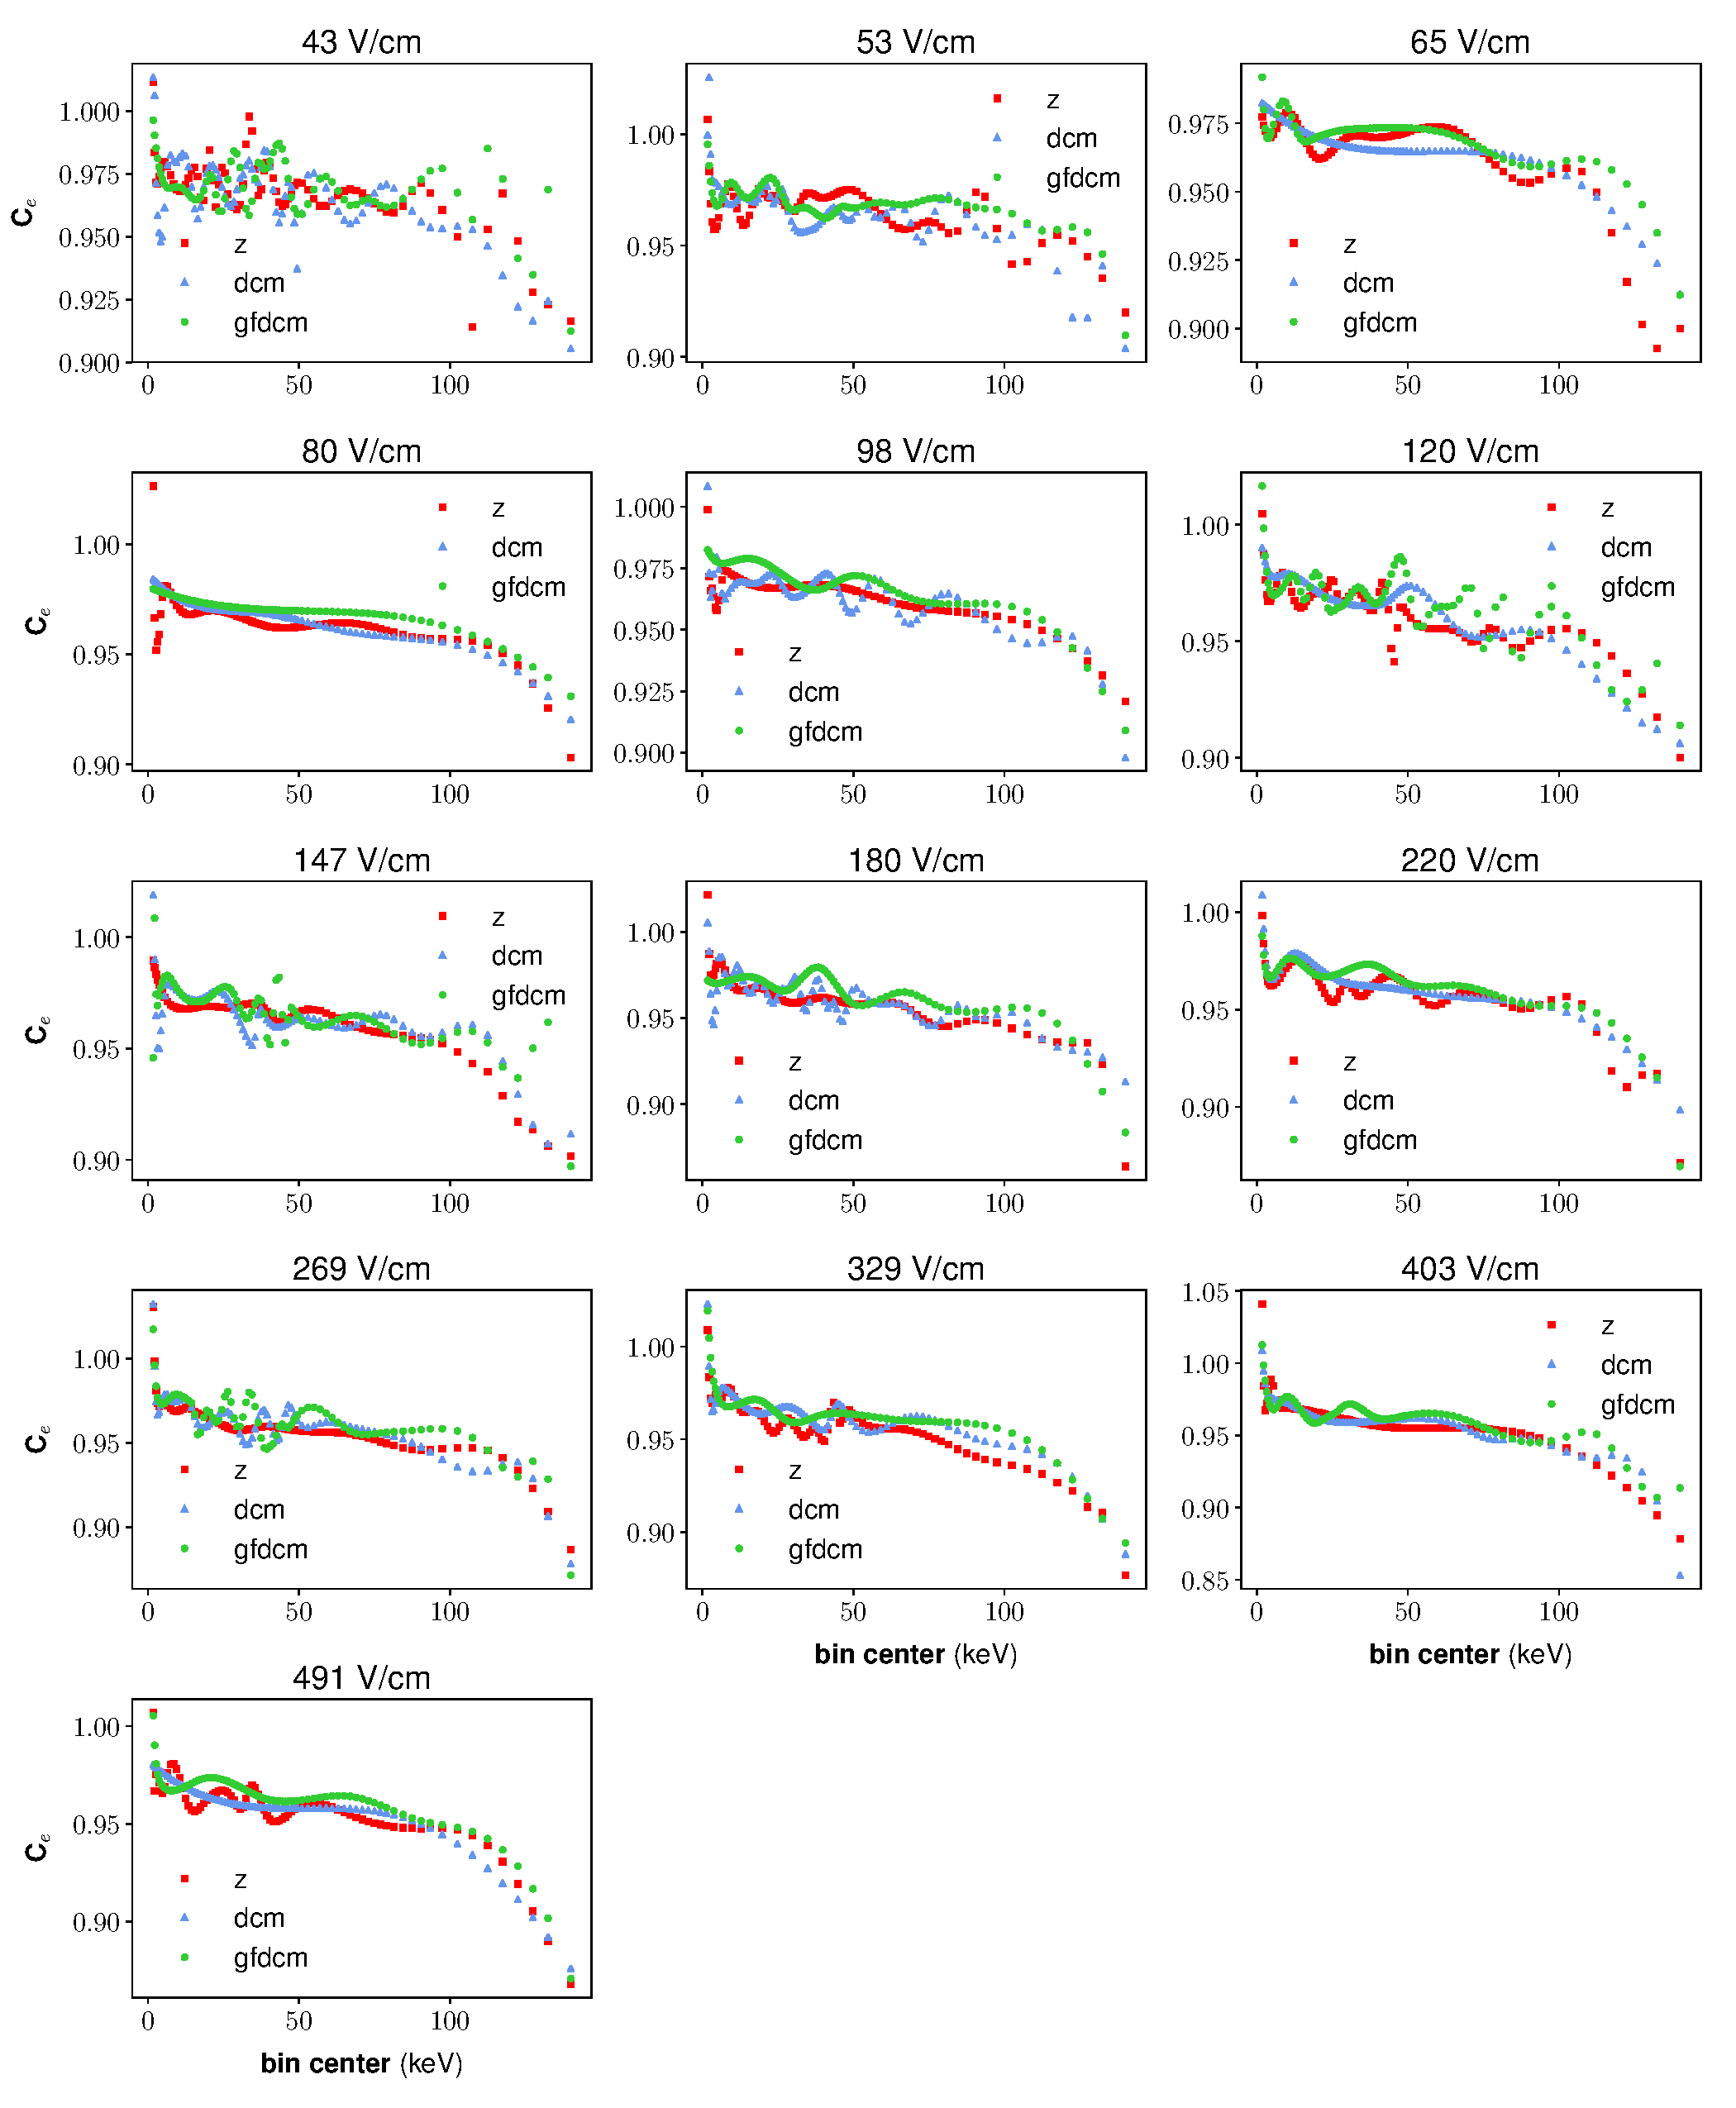
\includegraphics[width=\textwidth]{Figures/C14_CE_prelim.pdf}
\caption{Carbon-14 energy smearing correction factors for the three efficiency corrections being studied, in each of the electric field bins. The x-axis shows the central value the reconstructed energy bin for which the correction factor is calculated.}
\label{fig:C14_CE_prelim}
\end{figure}
\begin{figure}[h!]
\centering
\includegraphics[width=\textwidth]{Figures/C14_Ce_prelim.pdf}
\caption{Carbon-14 S2 smearing correction factors for the three efficiency corrections being studied, in each of the electric field bins. The x-axis shows the central value the reconstructed energy bin for which the correction factor is calculated.}
\label{fig:C14_Ce_prelim}
\end{figure}
The measured values of $QY_{ij}$ for all of the electric field bins is shown in figure \ref{fig:C14_QY_prelim}. The smearing corrections that go into calculating these values are shown in figures \ref{fig:C14_CE_prelim} and \ref{fig:C14_Ce_prelim}. We have shown the results measured using the three corrections-types described in section \ref{sec:corrections}; ``z'', ``dcm'', and ``gfdcm''. The ``gfdcm'' measurements of $QY$ are systematic higher than the other two corrections types and are more consistent with the Run03 values.

\begin{figure}[h!]
\centering
\begin{subfigure}{0.45\textwidth}
  \centering
  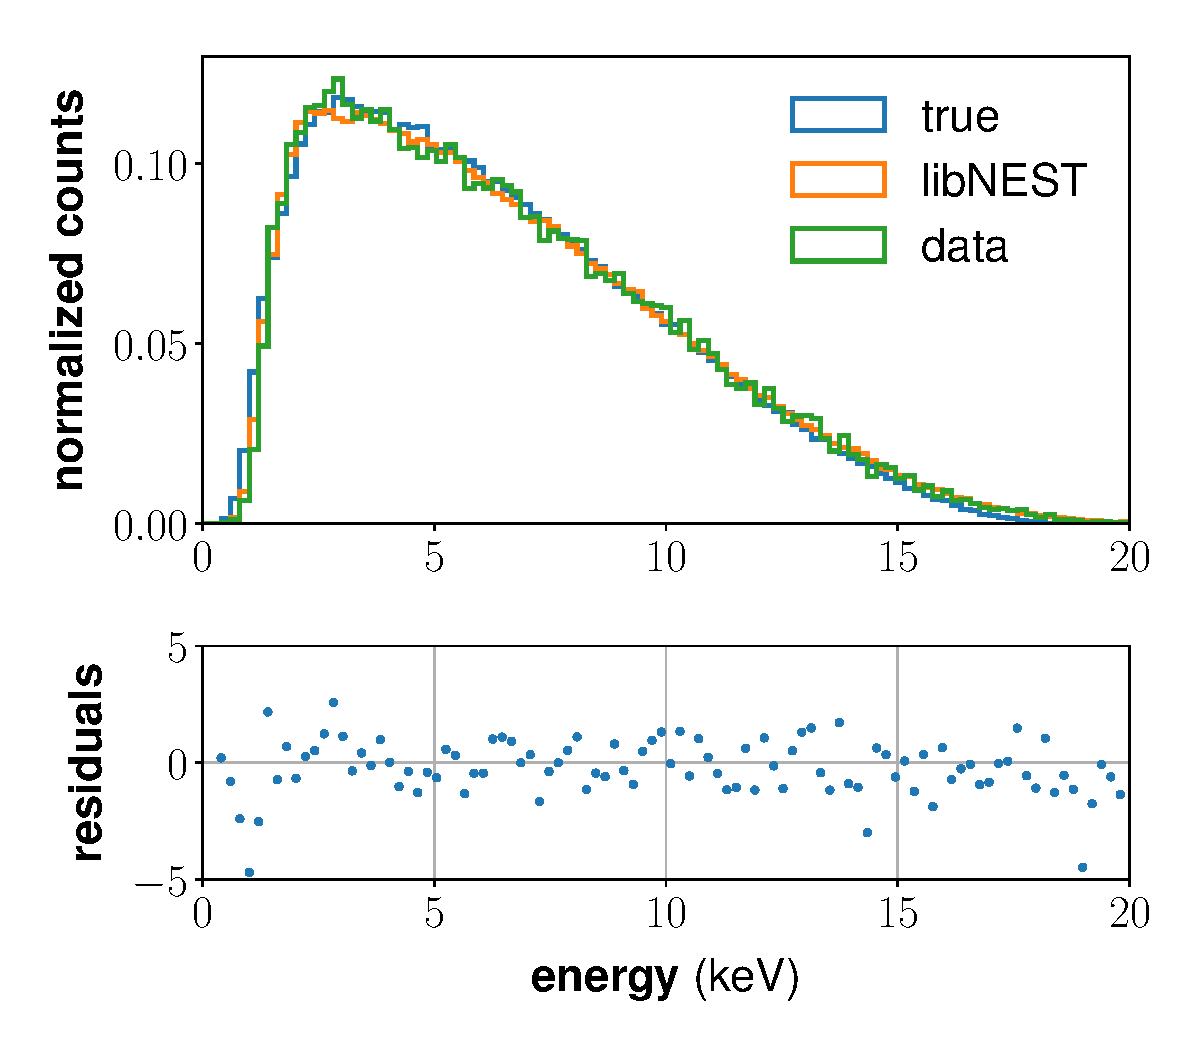
\includegraphics[width=\textwidth]{Figures/yields_corrections/H3_spectrum_gfdcm_180Vcm_prelim.pdf}
  \caption{}
\end{subfigure}%
\begin{subfigure}{0.45\textwidth}
  \centering
  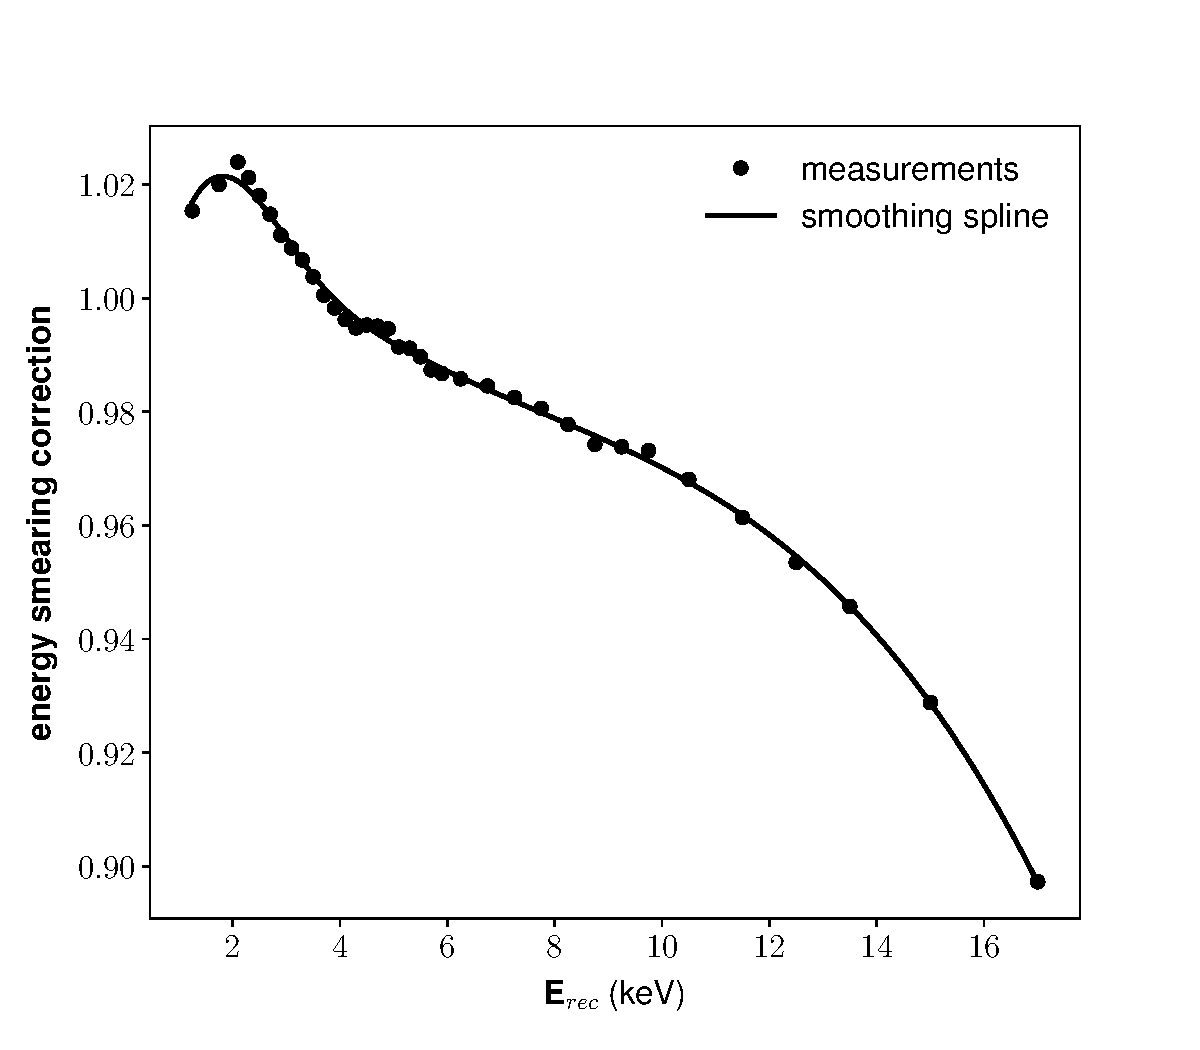
\includegraphics[width=\textwidth]{Figures/yields_corrections/H3_E_correction_gfdcm_180Vcm_prelim.pdf}
  \caption{}
\end{subfigure}
\begin{subfigure}{0.45\textwidth}
  \centering
  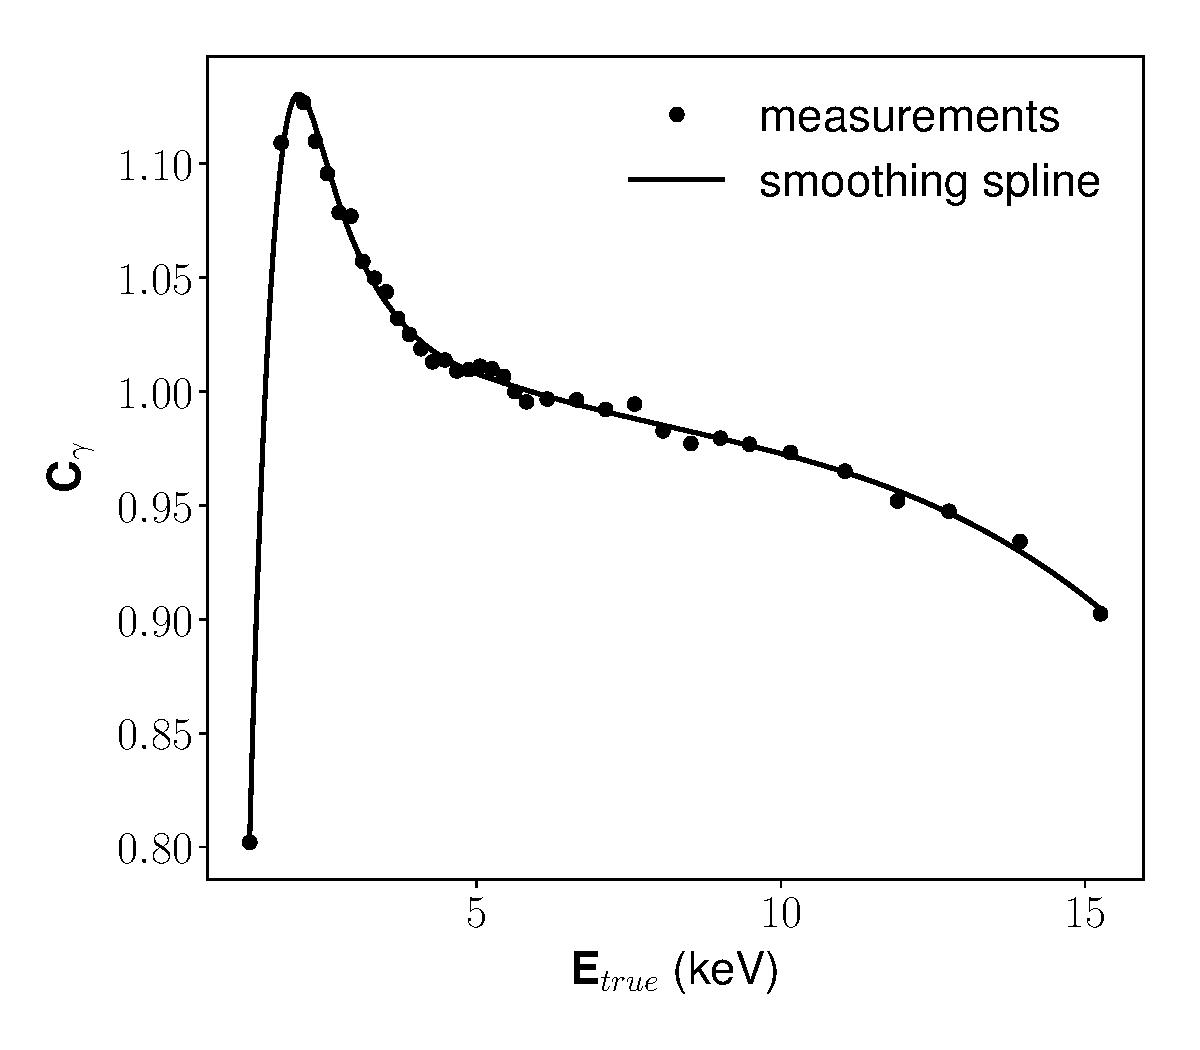
\includegraphics[width=\textwidth]{Figures/yields_corrections/H3_LN_correction_gfdcm_180Vcm_prelim.pdf}
  \caption{}
\end{subfigure}%
\begin{subfigure}{0.45\textwidth}
  \centering
  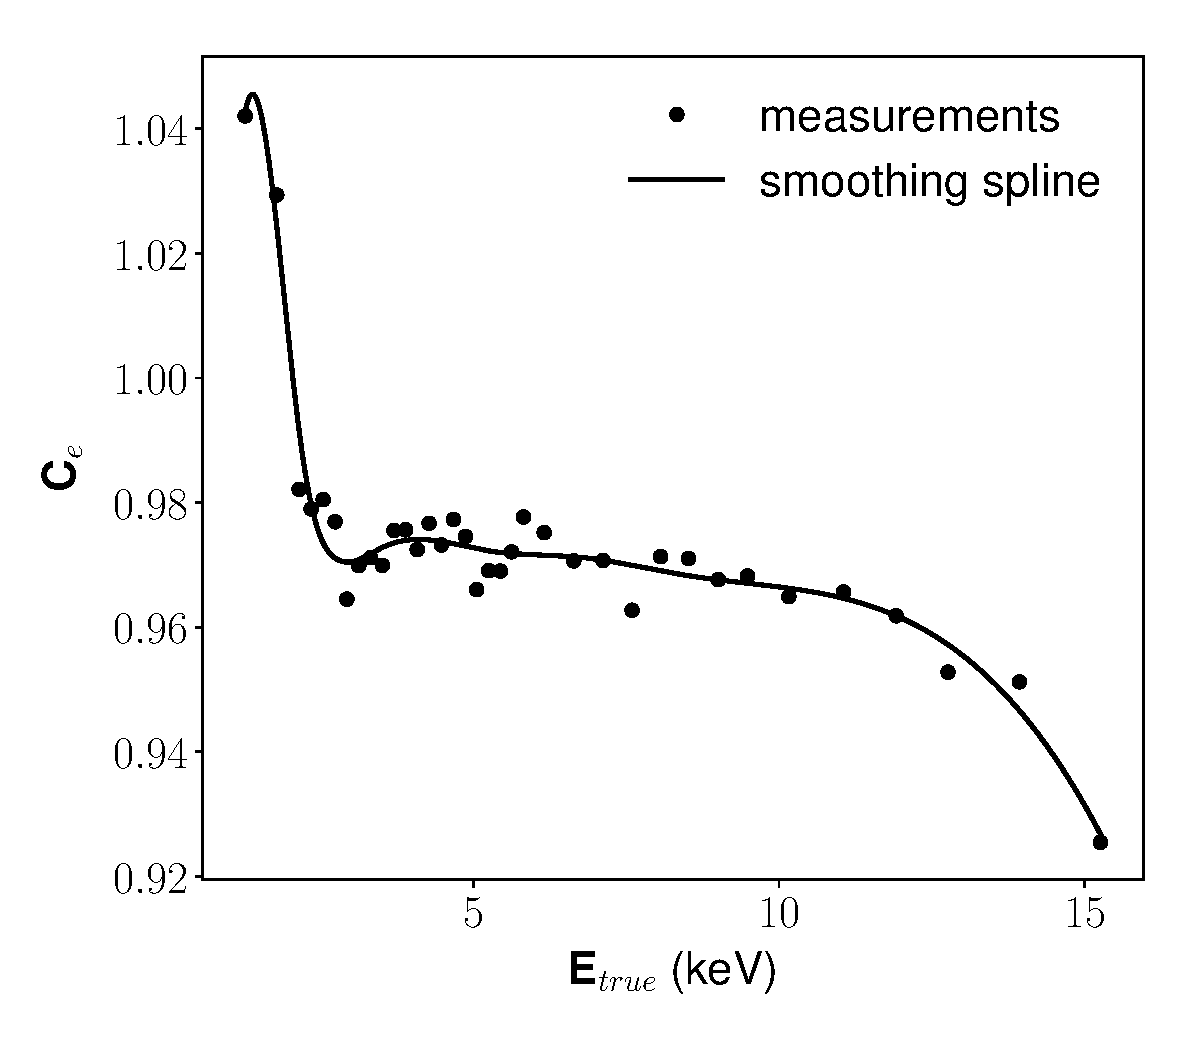
\includegraphics[width=\textwidth]{Figures/yields_corrections/H3_QN_correction_gfdcm_180Vcm_prelim.pdf}
  \caption{}
\end{subfigure}
\begin{subfigure}{0.45\textwidth}
  \centering
  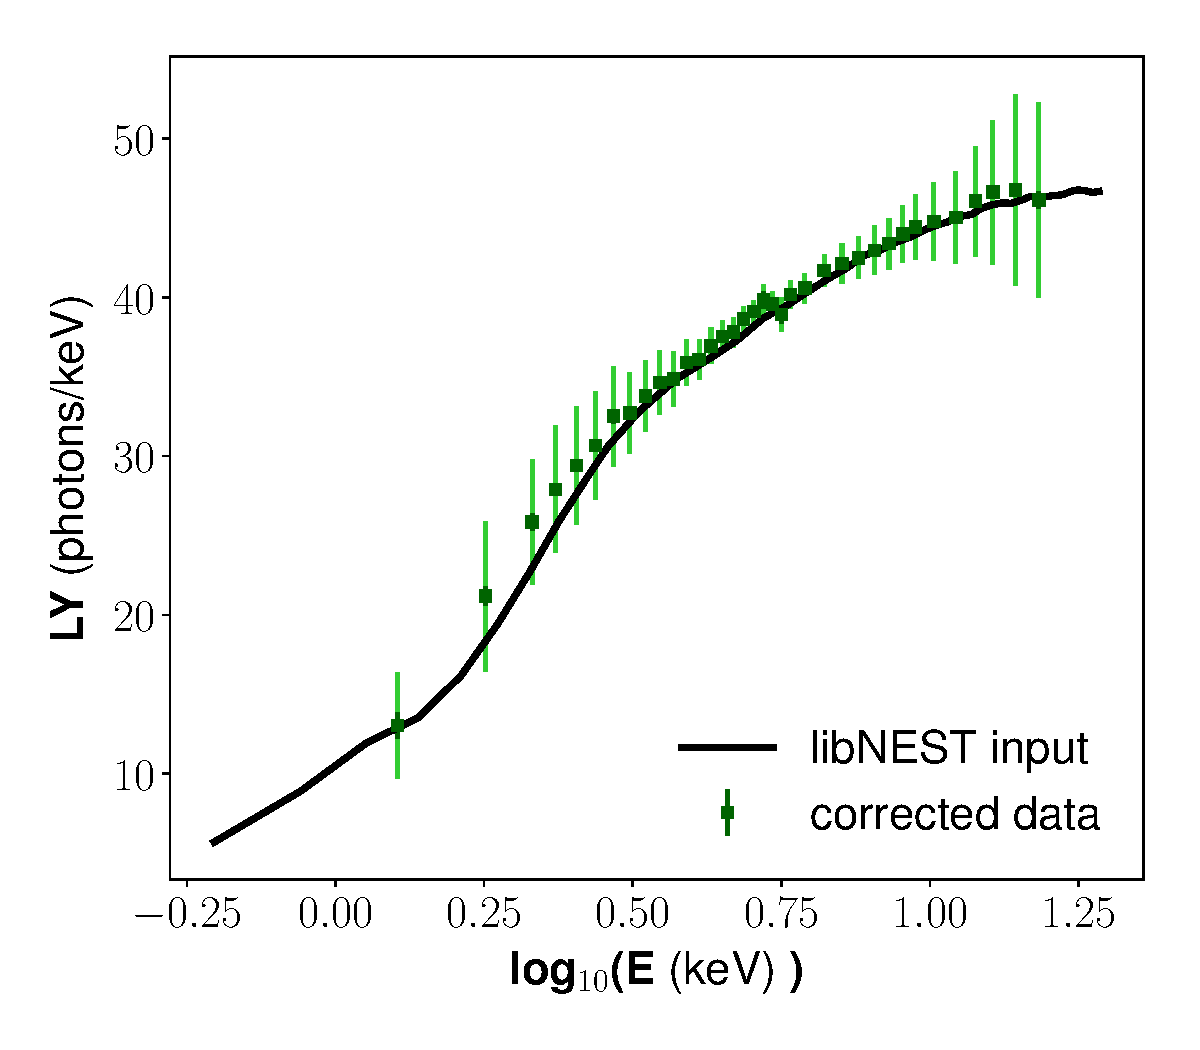
\includegraphics[width=\textwidth]{Figures/yields_corrections/H3_LY_final_gfdcm_180Vcm_prelim.pdf}
  \caption{}
\end{subfigure}%
\begin{subfigure}{0.45\textwidth}
  \centering
  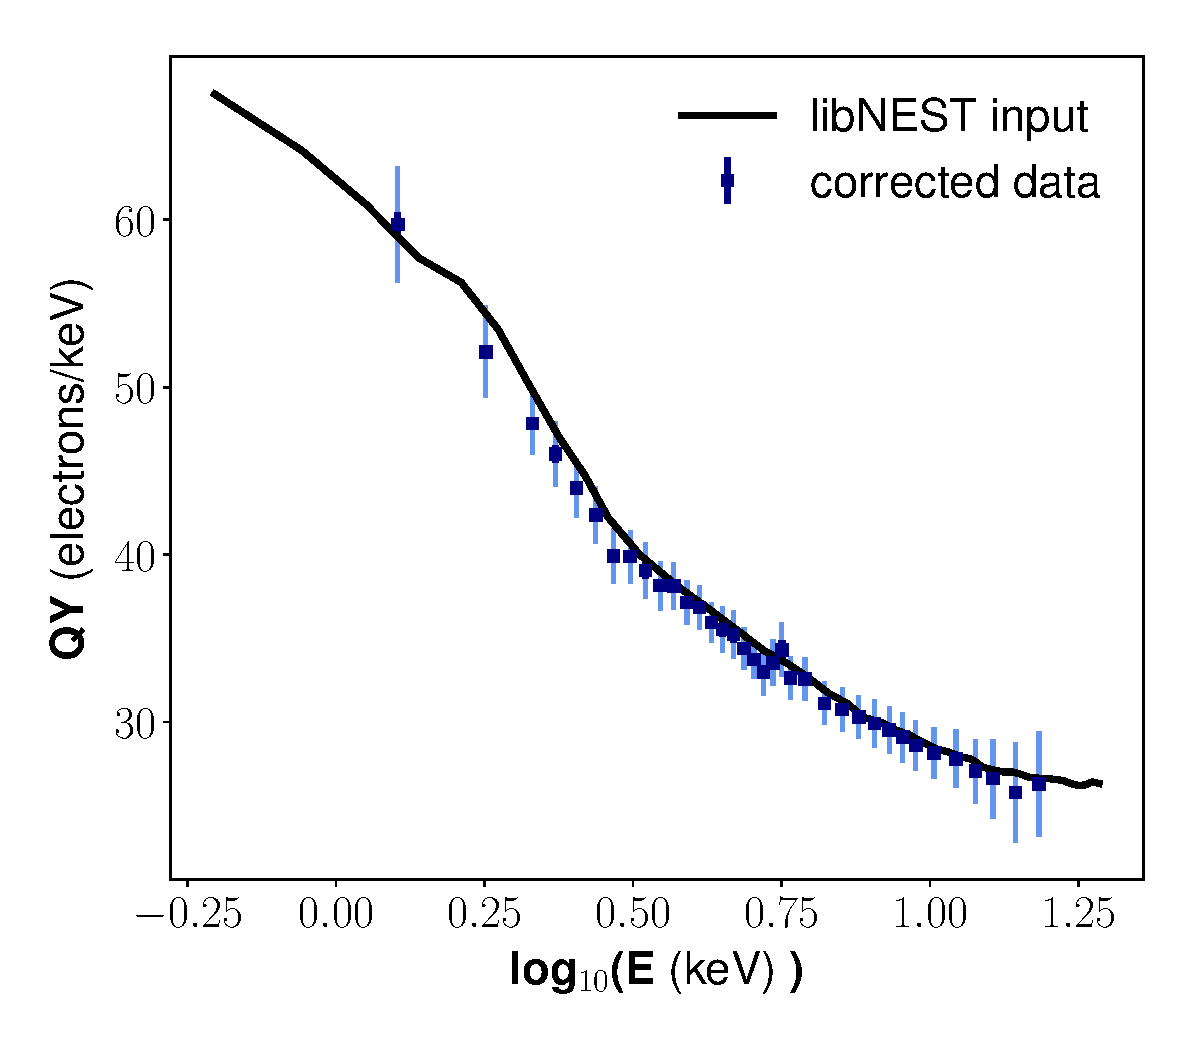
\includegraphics[width=\textwidth]{Figures/yields_corrections/H3_QY_final_gfdcm_180Vcm_prelim.pdf}
  \caption{}
\end{subfigure}
\caption{Calculations for preliminary tritium yields in the 180 V/cm drift bin, using the ``gfdcm'' data corrections. These plots are analogous to those previously shown for carbon-14.}
\label{fig:h3_180}
\end{figure}

The same procedure that was used for carbon-14 was also performed on the post-Run04 tritium data. The reconstructed energy bins used for tritium are described in table \ref{tab:ebins_h3}. The results for tritium in the 180 V/cm electric field bin are shown in figure. \ref{fig:h3_180}. The energy spectrum, including the threshold, is well modeled by libNEST. The reduced chi-squared difference between the libNEST and data spectra on an energy range from 0 to 20 keV is 1.5.

\begin{table}[h!]
\centering
    \begin{tabular}{ c || c | c | c | c | c  }
    \hline
    Energy Range (keV) & 1-2 & 2-6  & 6-10 & 10-14 & 14-18\\
    \hline
    Bin Width (keV)         &  0.5       & 0.2      &  0.5         & 1           & 2 \\
    \hline
    \end{tabular}
    \caption{Tritium reconstructed energy bin widths and their associated energy ranges.}
    \label{tab:ebins_h3}
\end{table}

\begin{figure}[h!]
\centering
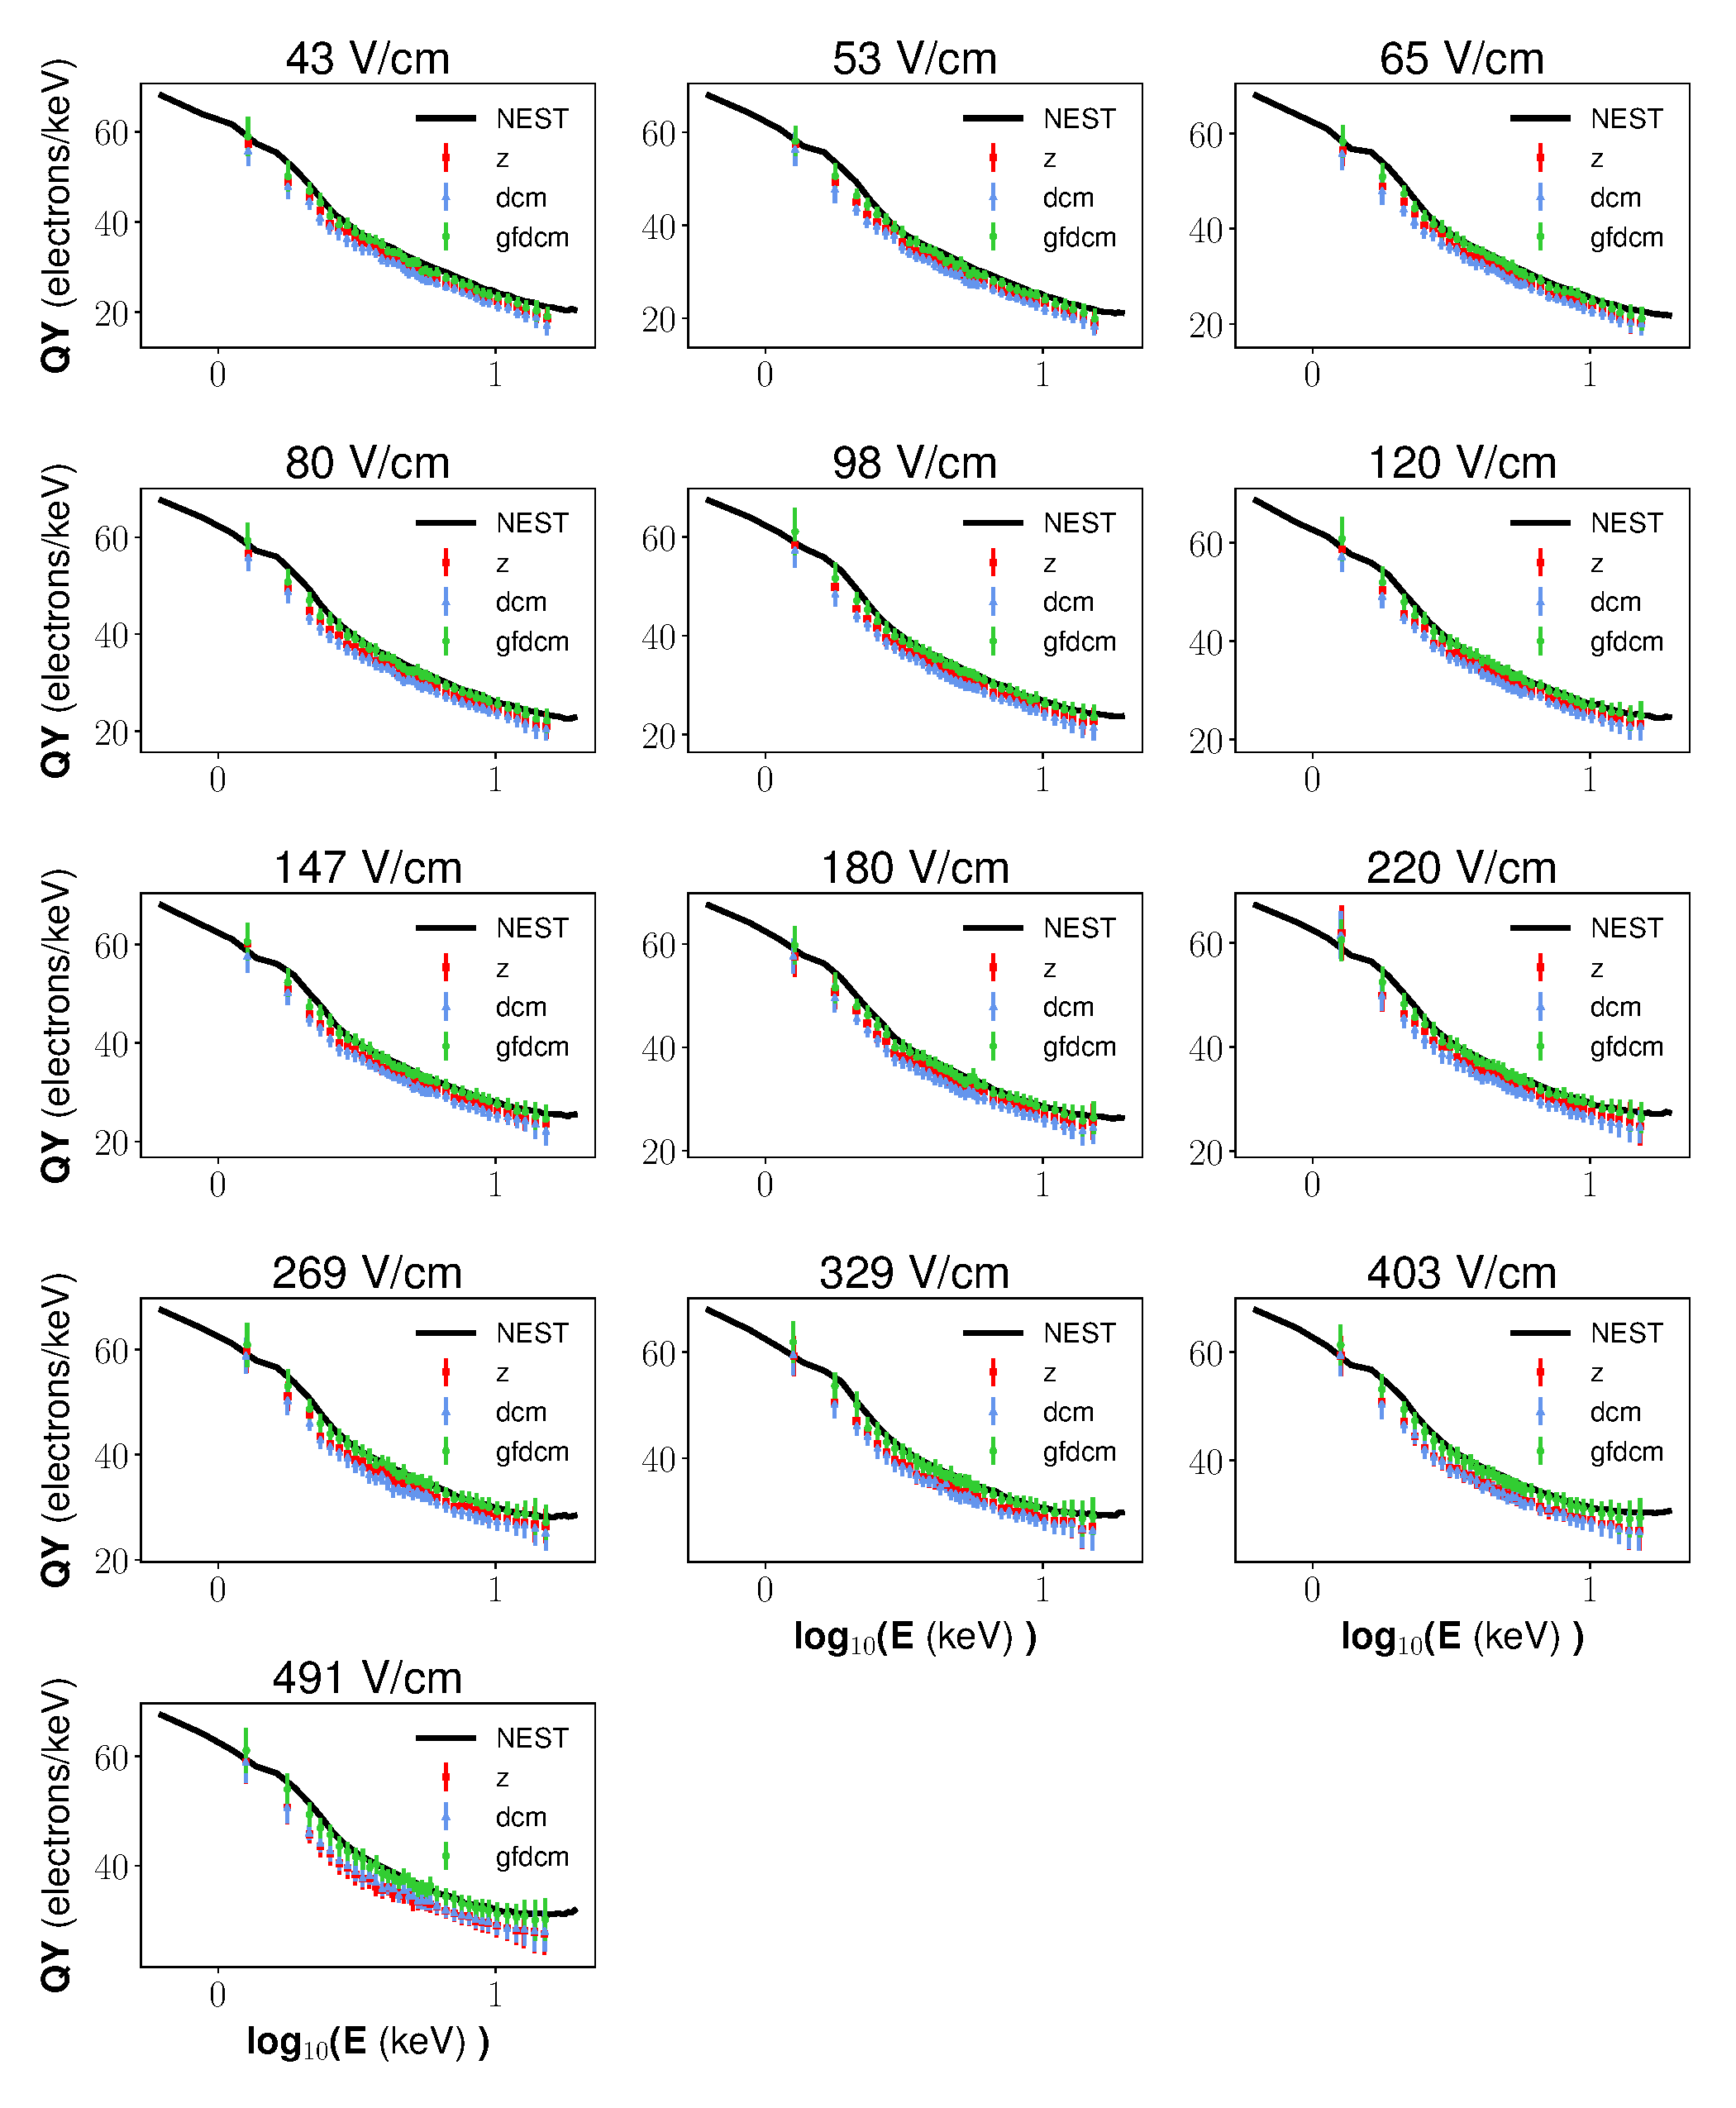
\includegraphics[width=\textwidth]{Figures/H3_QY_prelim.pdf}
\caption{Preliminary tritium charge yield for the three efficiency corrections being studied, in each of the 13 electric field bins defined in \ref{sec:fieldbins}. The x-axis here represents the true event energy, obtained by applying the smearing corrections. The charge yields measured here will be used to fine-tune the NEST model in order to obtain a more accurate set of corrections.}
\label{fig:H3_QY_prelim}

\end{figure}

The smearing corrections are obtained in the same way as for carbon-14. The effect of the threshold on the smearing corrections can be most clearly seen in the first few energy bins, where $C_{\gamma}$ drops sharply from about 0.8 to 1.1 in the space of two energy bins. The S2 correction, $C_{e}$, also sees a large jump in these bins; it falls from about 1.4 to 0.98. The resulting charge yield measurements are in good agreement both with those for carbon-14 and with the existing libNEST model. In the next section, we will combine the charge yields from carbon-14 and tritium with measurements from other experiments in order to find an equation for $QY_{NEST}(E,\mathcal{E})$.

\begin{figure}[h!]
\centering
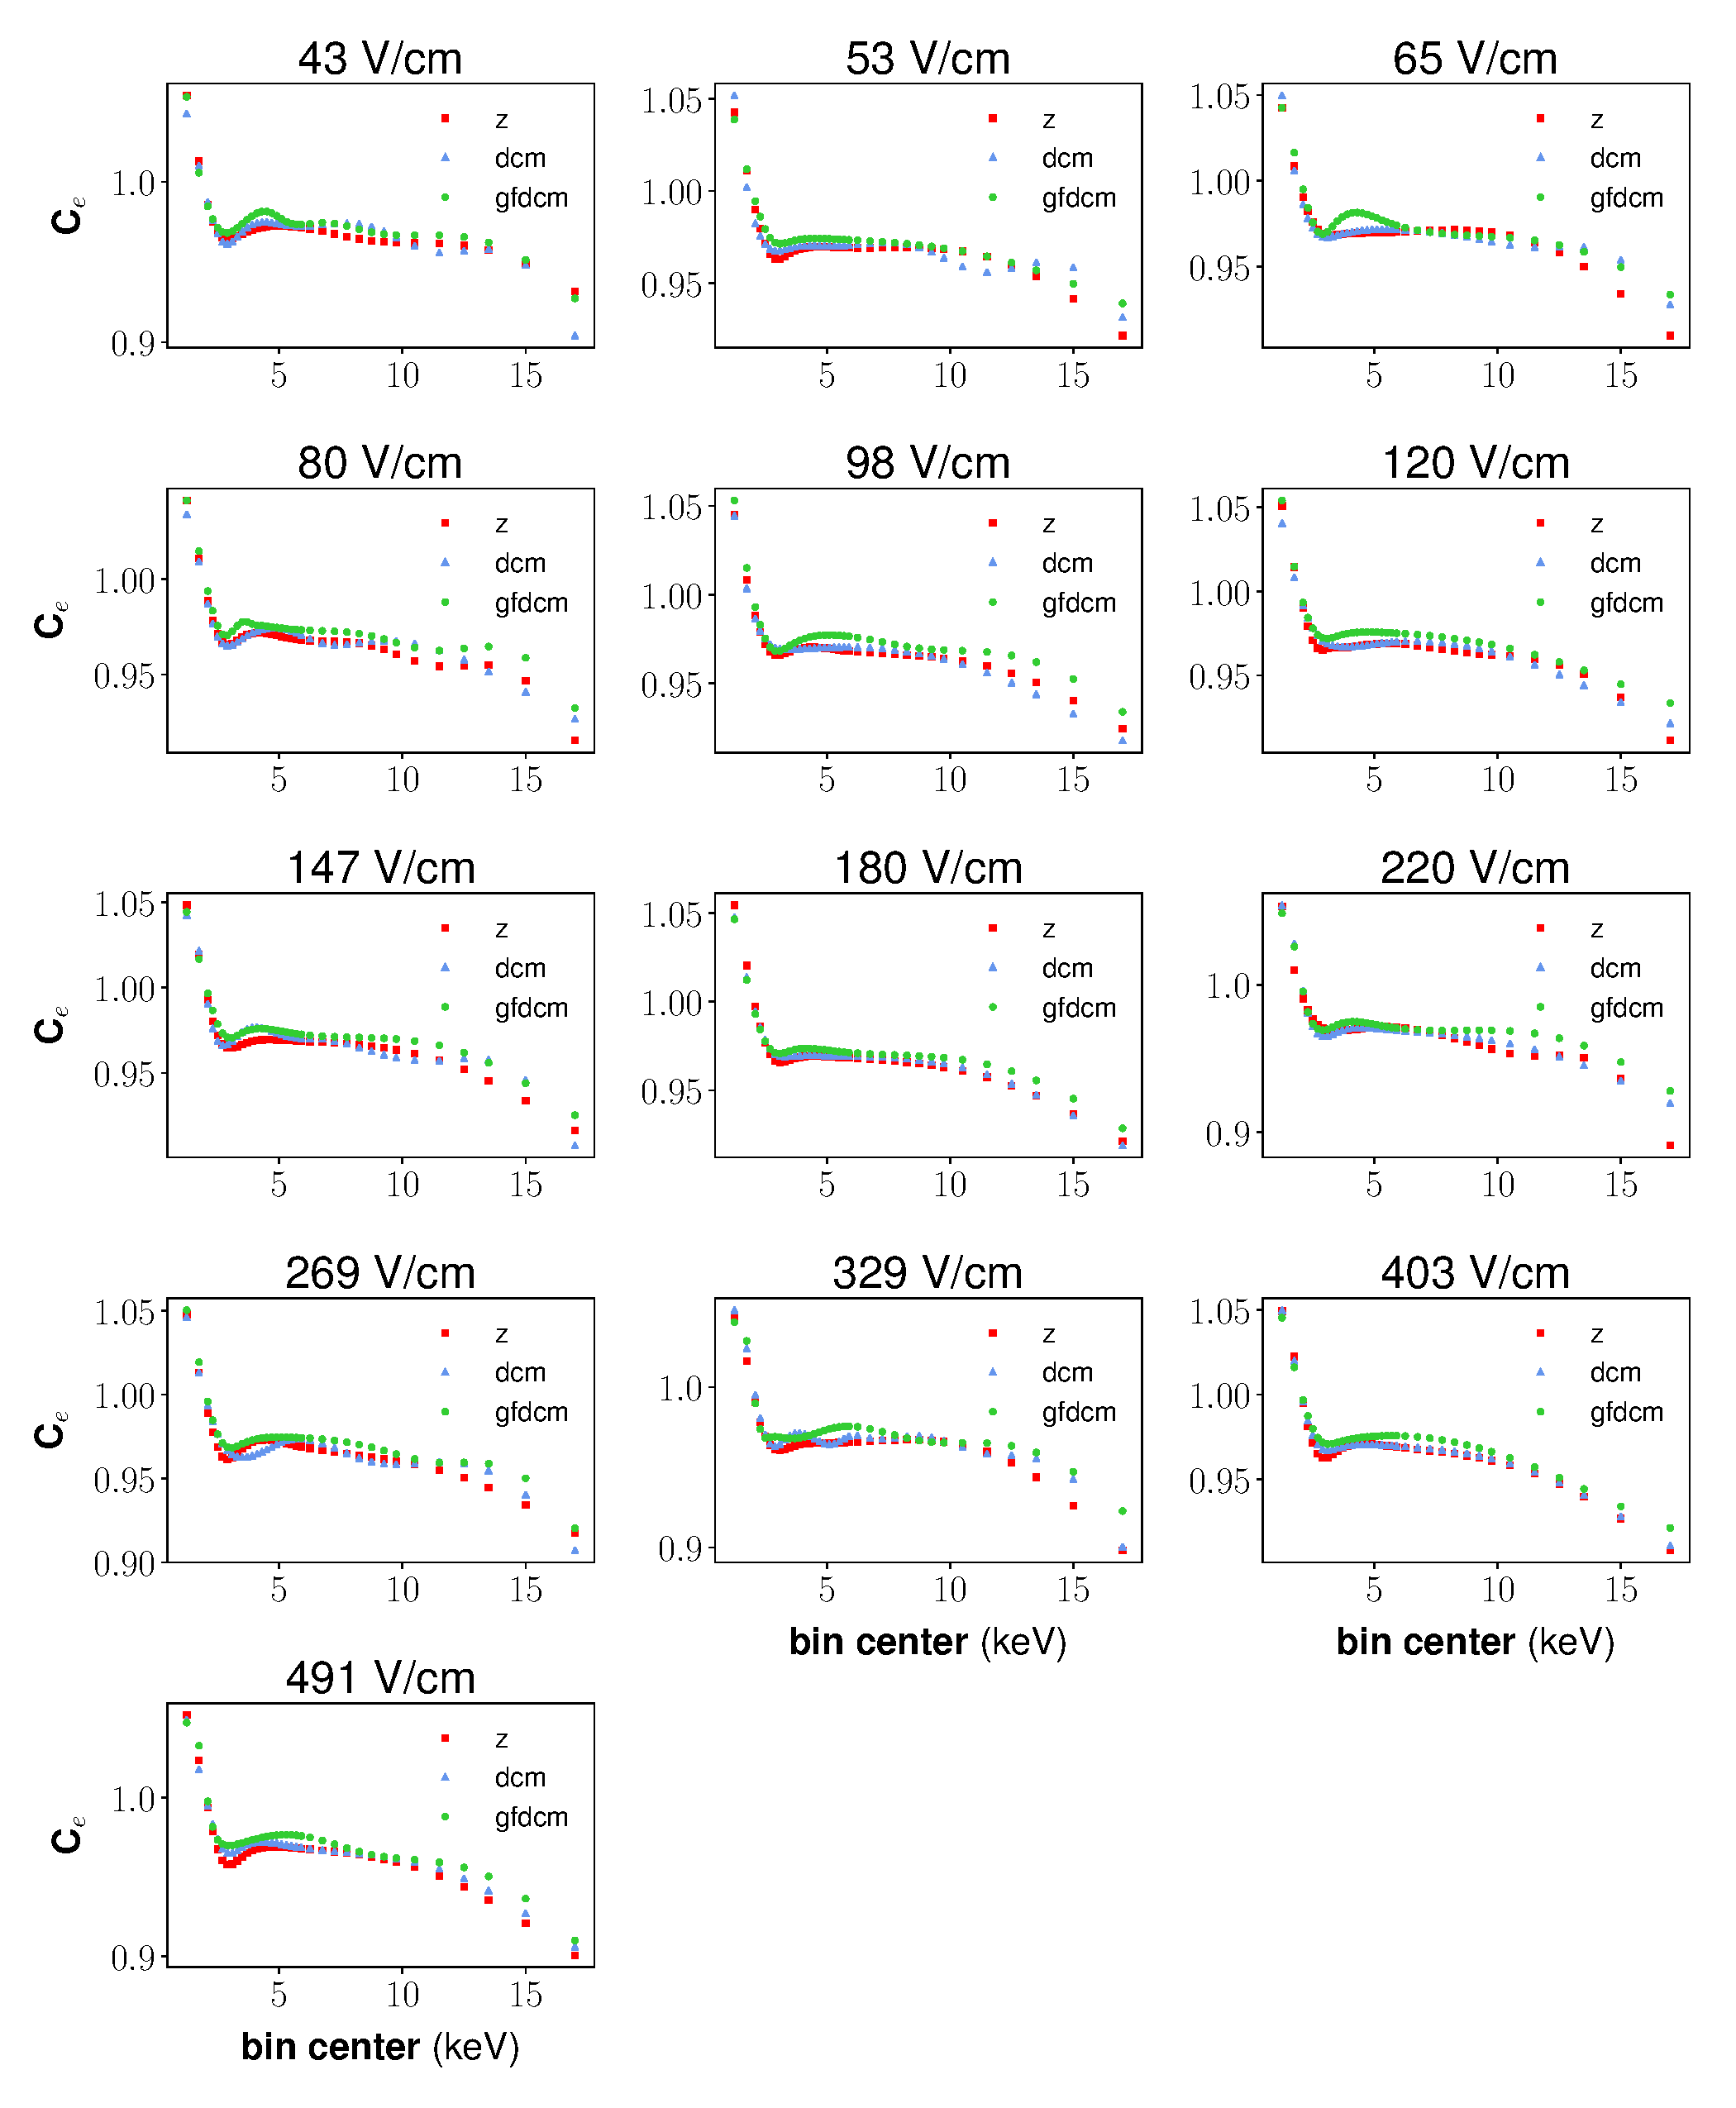
\includegraphics[width=\textwidth]{Figures/H3_CE_prelim.pdf}
\caption{Tritium energy smearing correction factors for the three efficiency corrections being studied, in each of the electric field bins. The x-axis shows the central value the reconstructed energy bin for which the correction factor is calculated.}
\label{fig:H3_CE_prelim}
\end{figure}
\begin{figure}[h!]
\centering
\includegraphics[width=\textwidth]{Figures/H3_Ce_prelim.pdf}
\caption{Tritium energy smearing correction factors for the three efficiency corrections being studied, in each of the electric field bins. The x-axis shows the central value the reconstructed energy bin for which the correction factor is calculated.}
\label{fig:H3_Ce_prelim}
\end{figure}


\subsection{Preliminary Energy- and Field-Dependent Charge Yield Model}\label{sec:qyprelim}
The first step in finding an expression for $QY_{NEST}(E,\mathcal{E})$ is to choose a functional form. Historically, NEST has relied heavily on sigmoids to express the energy and field dependence of physical quantities:
\begin{equation}\label{eq:sigmoid}
F(x)=p_1+\frac{p_2-p_1}{1+(x/p_3)^{p_4}}
\end{equation}
For the purpose of characterizing the charge yield, we found that a combination of two asymmetric sigmoids is best able to reproduce the measurements at all fields and energies:
\begin{equation}
QY_{NEST}(E,\mathcal{E})|_{\mathcal{E}_1}=m_1+\frac{m_2-m_1}{(1+(E/m_3)^{m_4})^{m_9}}+m_5+\frac{0-m_5}{(1+(E/m_7)^{m_8})^{m_{10}}},
\end{equation}
where $m_1$ through $m_10$ will be allowed to vary with electric field. The $m_6$ parameter is set to 0 in order to break degeneracy. The $m_9$ and $m_10$ are oddly defined in this equation because they were a later addition after fits to a double symmetric sigmoid failed to produce good enough results. The remaining nonzero parameters will be fit to the preliminary measurements of $QY$ versus $\langle E_{true} \rangle$ in each of the electric field bins, giving us a set of 13 measurements for each parameter. 
\begin{figure}[h!]
\centering
\begin{subfigure}{0.45\textwidth}
  \centering
  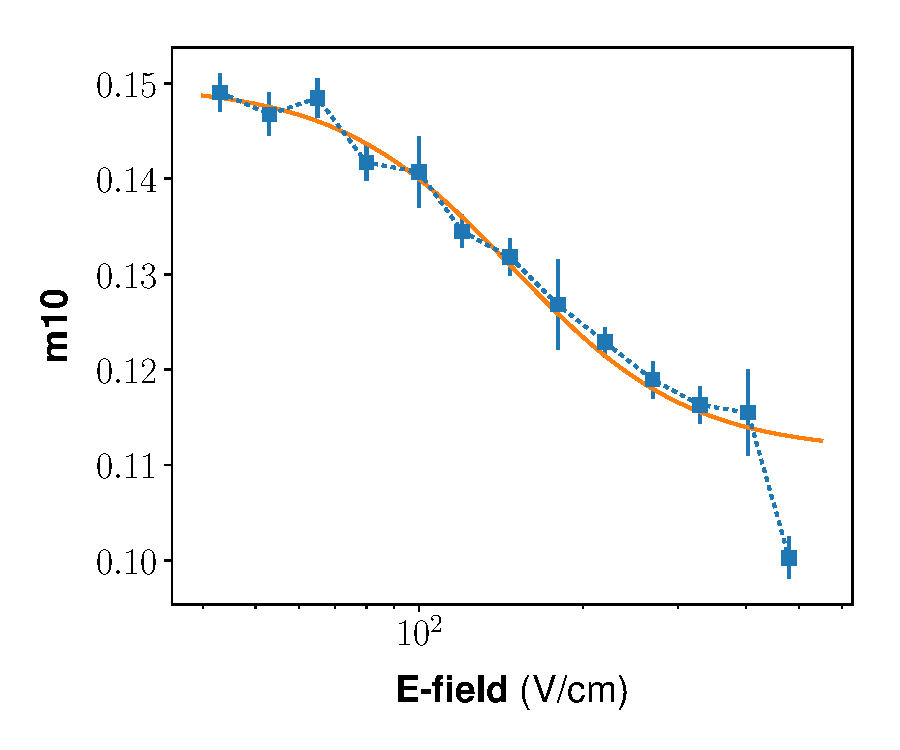
\includegraphics[width=\textwidth]{Figures/Yields_fit_old/NEST_m10_fit_old.pdf}
  \caption{}
\end{subfigure}%
\begin{subfigure}{0.45\textwidth}
  \centering
  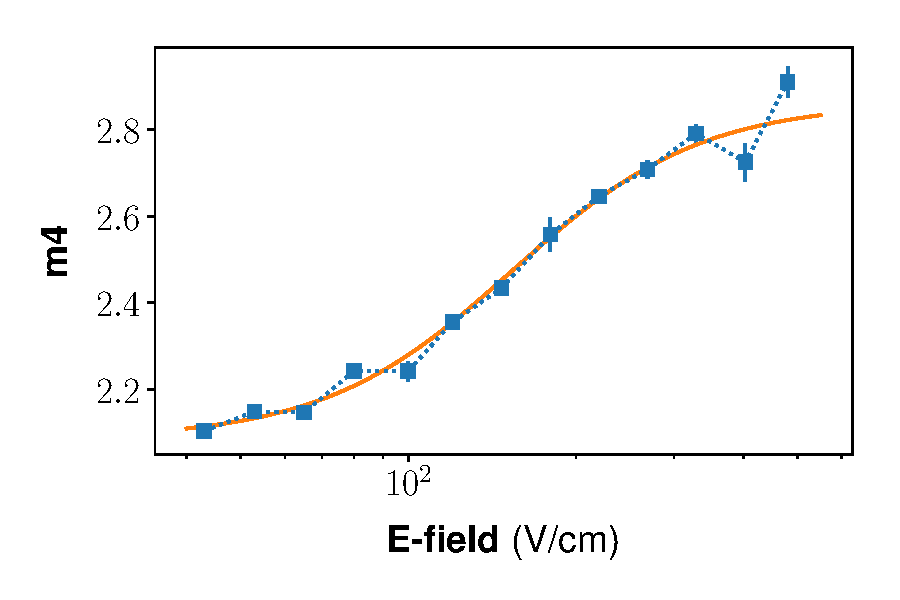
\includegraphics[width=\textwidth]{Figures/Yields_fit_old/NEST_m4_fit_old.pdf}
  \caption{}
\end{subfigure}
\begin{subfigure}{0.45\textwidth}
  \centering
  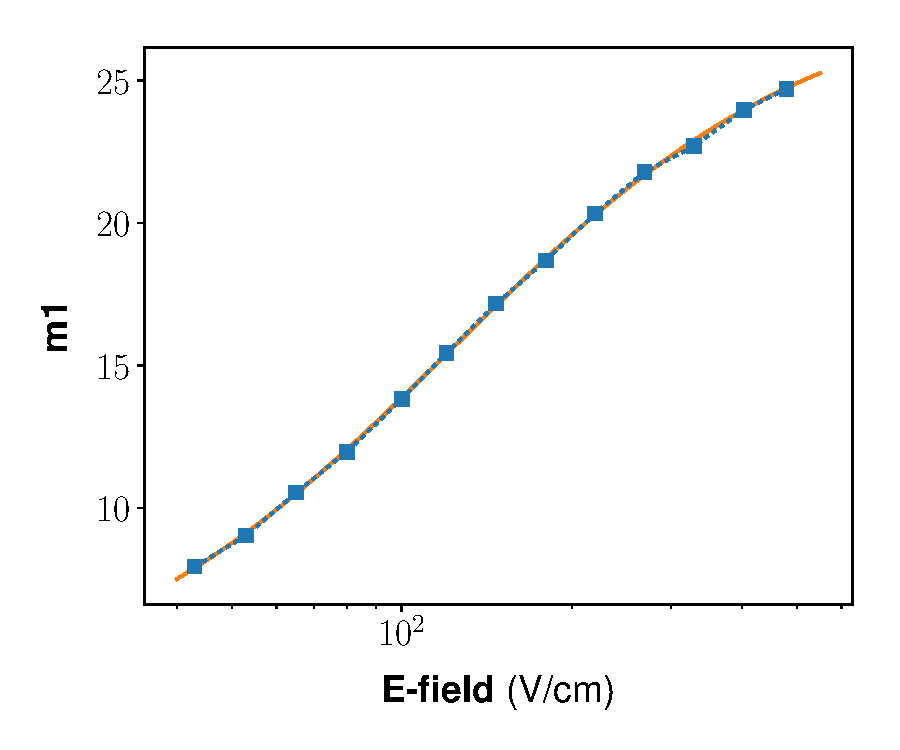
\includegraphics[width=\textwidth]{Figures/Yields_fit_old/NEST_m1_fit_old.pdf}
  \caption{}
\end{subfigure}%
\begin{subfigure}{0.45\textwidth}
  \centering
  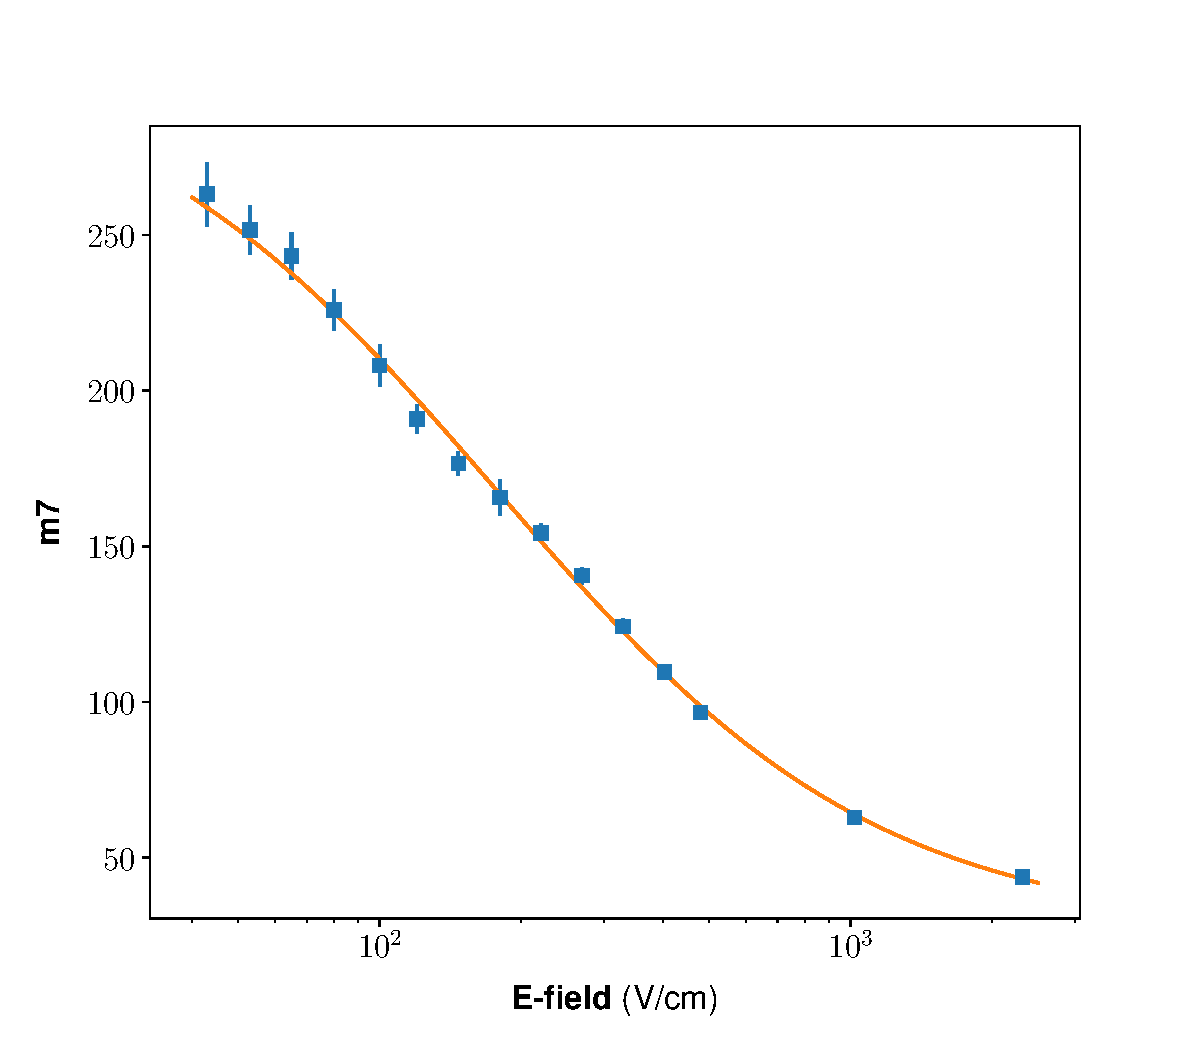
\includegraphics[width=\textwidth]{Figures/Yields_fit_old/NEST_m7_fit_old.pdf}
  \caption{}
\end{subfigure}
\caption{Sigmoid fits to the $QY$ parameters which could not be held constant. The blue markers show the measured parameters for the ``gfdcm'' data. The orange lines show fits to the parameters as functions of electric field.}
\label{fig:gfdcm_prelim_params}
\end{figure}

We first fit to the measurements from the ``gfdcm'' data and found that the $m_8$ parameter (among others) was roughly constant over all the field bins. We repeated the fit holding $m_8$ equal to the error-weighted average of 4.00. After obtaining a new set of best-fit parameters, we repeated the fit again this time also holding $m_9$ to its average value of 0.288. We repeated this process for $m_2=76.9$, $m_5=37.5$, and $m_3=0.837$, but after this point all of the remaining parameters had clear trends in electric field. Each remaining parameter's trend in electric field was fit to a single symmetric sigmoid, as shown in equation \ref{eq:sigmoid}.
\begin{figure}[h!]
  \centering
  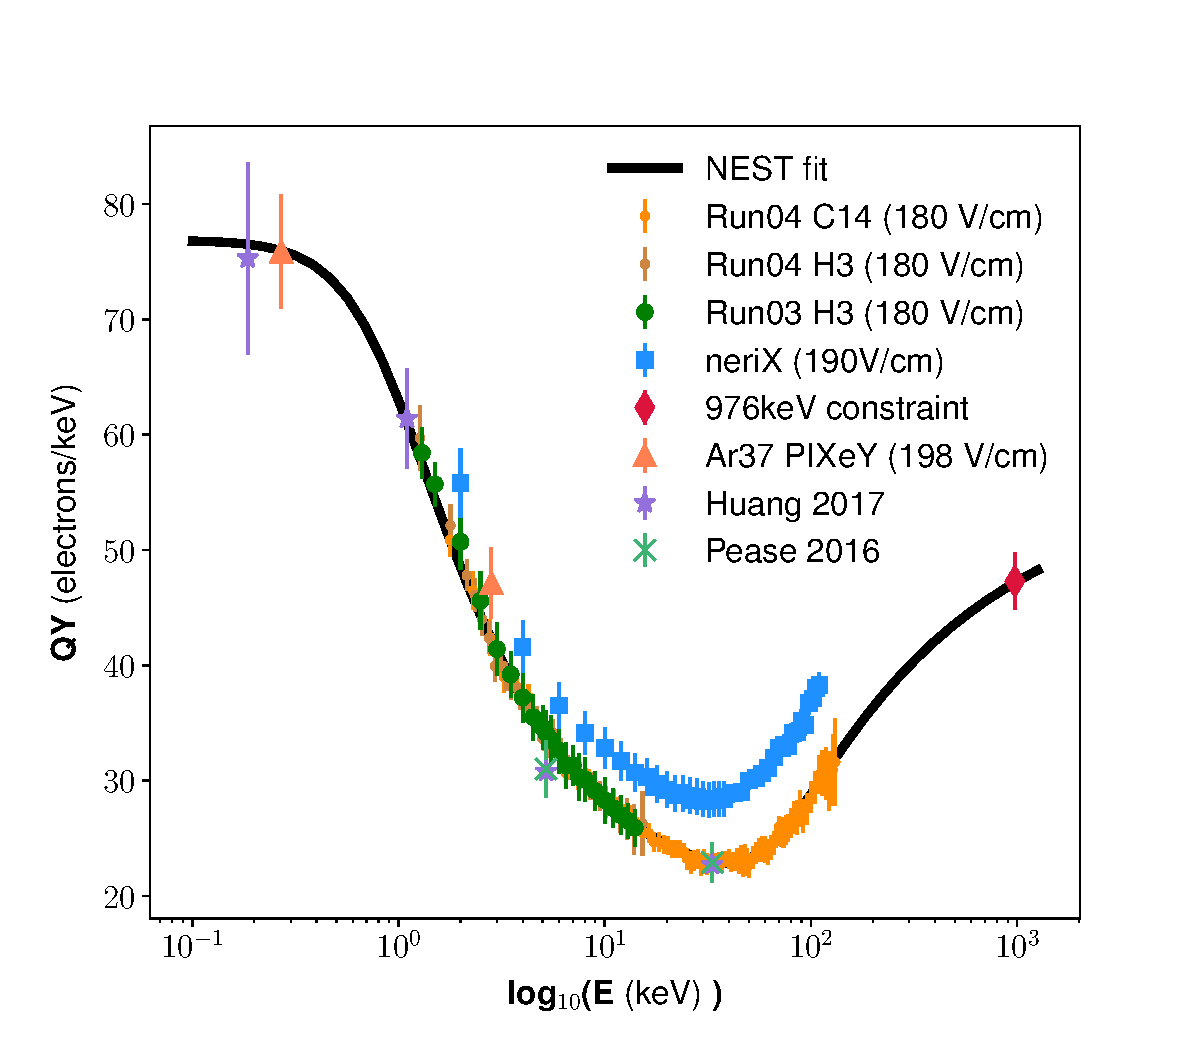
\includegraphics[width=\textwidth]{Figures/Yields_fit_old/NEST_fit_180Vcm_old.pdf}
  \caption{Best fit $QY$ for ``gfdcm'' data in the 180 V/cm electric field bin. The orange points are the post-Run04 carbon-14 measurements, and the brown points are the post-Run04 tritium measurements. The datasets labeled ``Run03 H3'', ``Huang 2017'', and ``Pease 2017'' are all from LUX Run03 measurements. The blue squares are not included in the fit. The other datasets are described in section \ref{sec:NESTbeta}.}
  \label{fig:gfdcm_prelim_QY180}
\end{figure}

Figure \ref{fig:gfdcm_prelim_QY180} the best-fit function for the 180 V/cm field bin. The brown and orange points show the ``gfdcm'' $QY$ data for post-Run04 tritium and carbon-14, respectively. The other data shown is used most to constrain the high and low energy regions of the fit. The lavender stars, teal ``X's'', and green markers are all from LUX Run03 \cite{lux_tritium, DQyields, Evanyields}. The Run03 and post-Run04 measurements are all in good agreement. The blue square markers are from measurements of Compton scattering in neriX detector\cite{nerix}. We do not include these points in the preliminary fits, but we will incorporate them when developing a final model of the yields. The full set of measurements will be discussed in detail in section \ref{sec:NESTNESTbeta}.
\begin{figure}[h!]
\centering
\begin{subfigure}{0.5\textwidth}
  \centering
  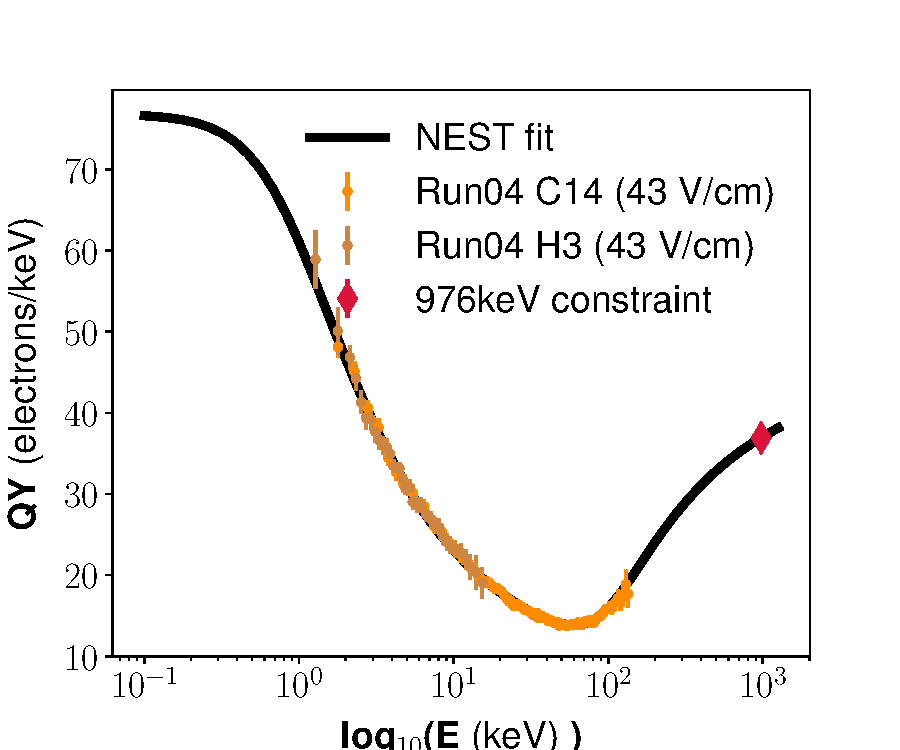
\includegraphics[width=\textwidth]{Figures/Yields_fit_old/NEST_fit_43Vcm_old.pdf}
  \caption{}
\end{subfigure}%
\begin{subfigure}{0.5\textwidth}
  \centering
  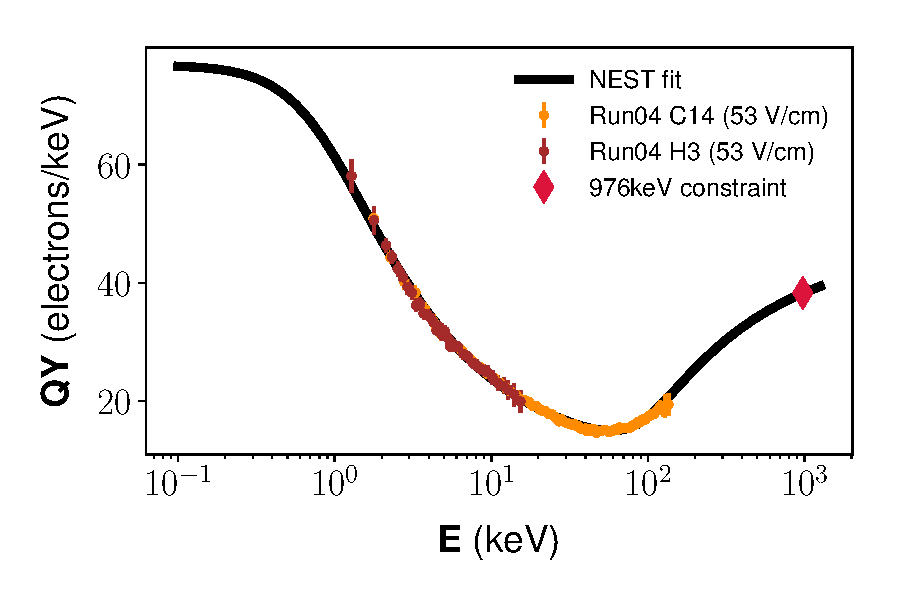
\includegraphics[width=\textwidth]{Figures/Yields_fit_old/NEST_fit_53Vcm_old.pdf}
  \caption{}
\end{subfigure}
\begin{subfigure}{0.5\textwidth}
  \centering
  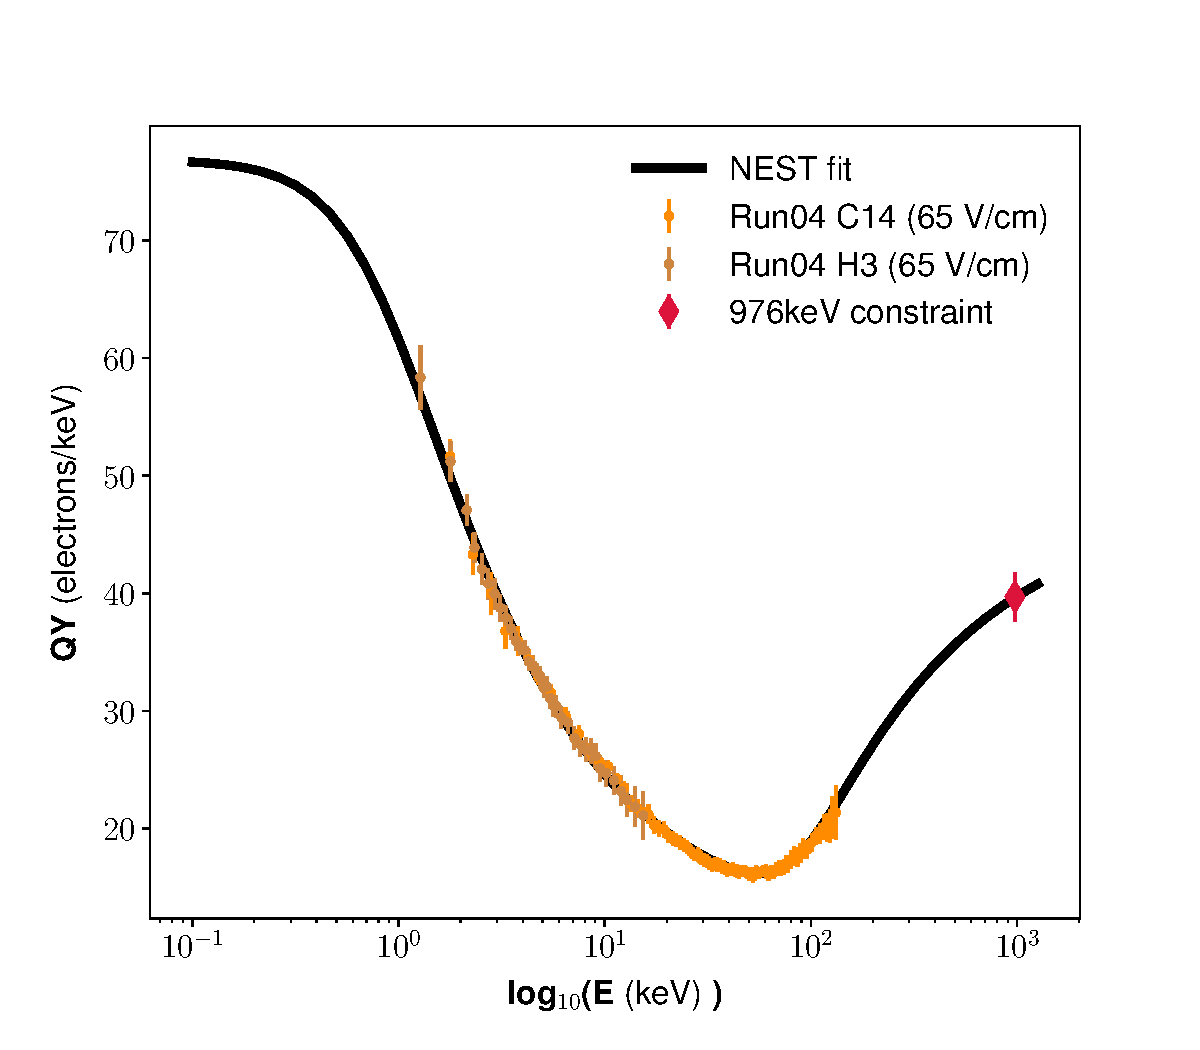
\includegraphics[width=\textwidth]{Figures/Yields_fit_old/NEST_fit_65Vcm_old.pdf}
  \caption{}
\end{subfigure}%
\begin{subfigure}{0.5\textwidth}
  \centering
  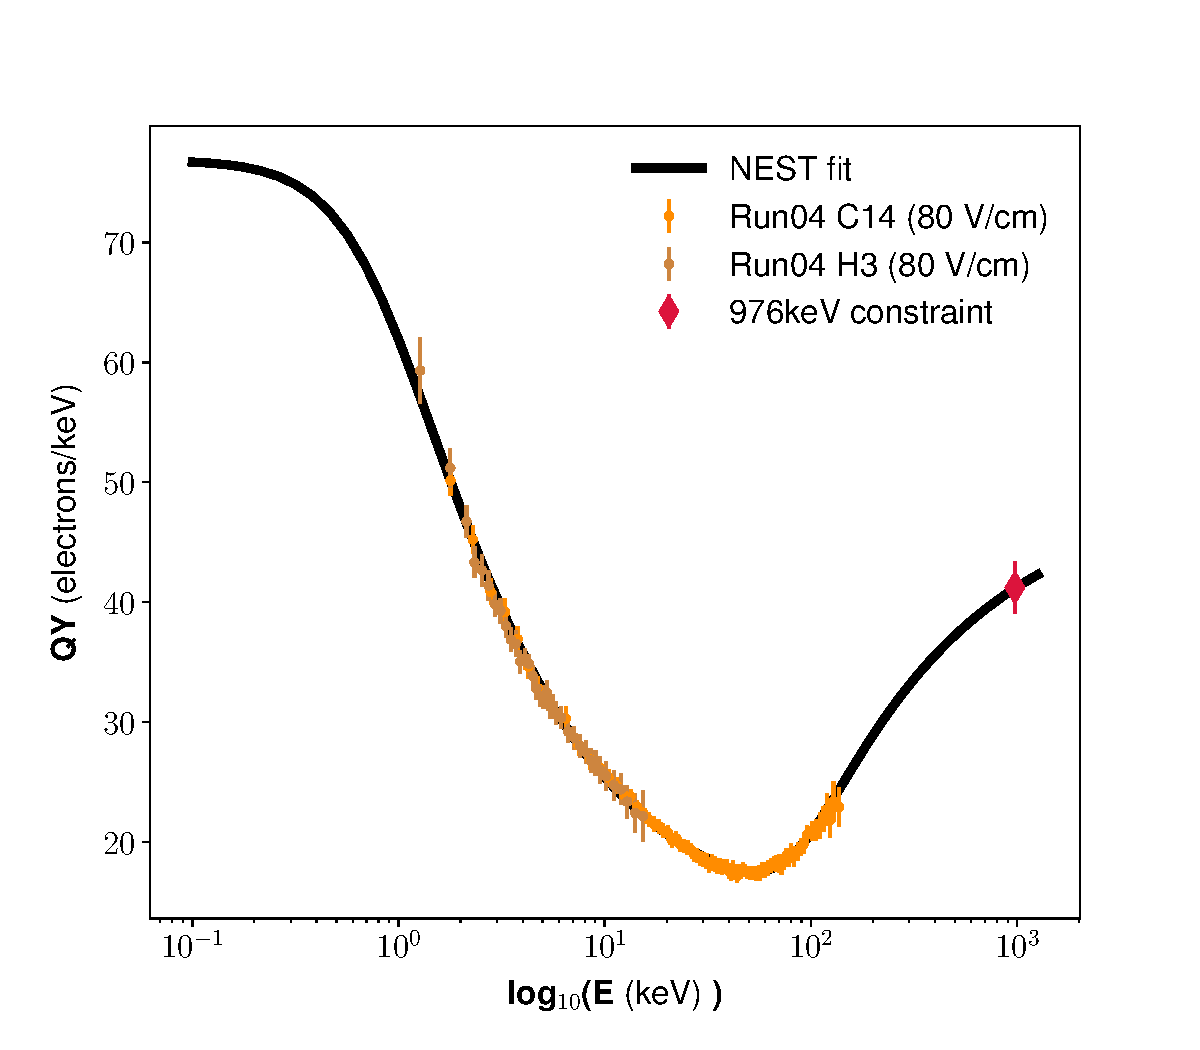
\includegraphics[width=\textwidth]{Figures/Yields_fit_old/NEST_fit_80Vcm_old.pdf}
  \caption{}
\end{subfigure}
\begin{subfigure}{0.5\textwidth}
  \centering
  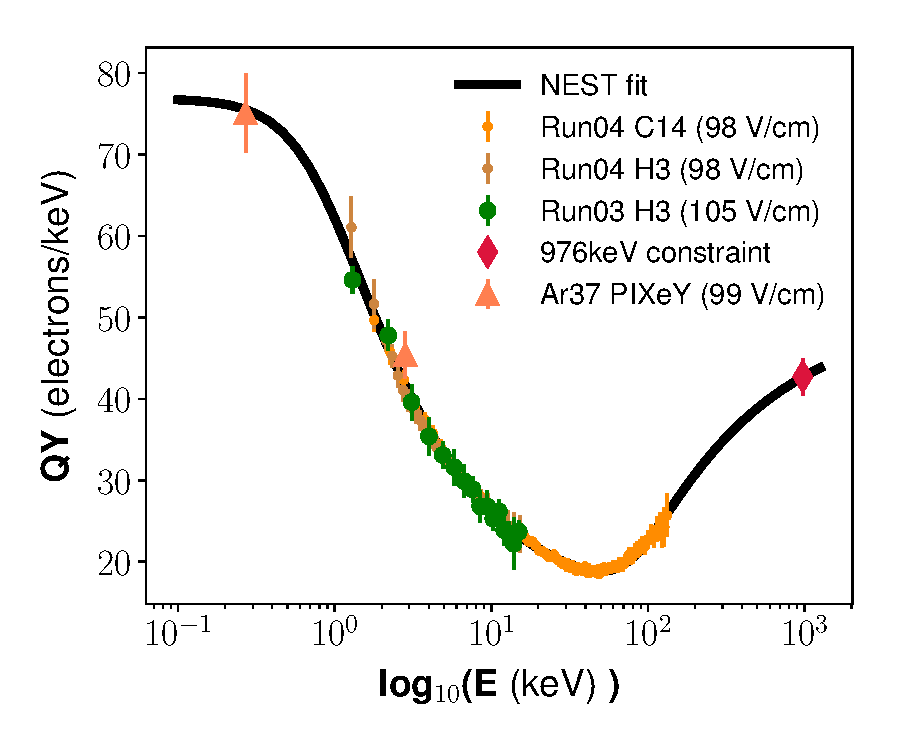
\includegraphics[width=\textwidth]{Figures/Yields_fit_old/NEST_fit_98Vcm_old.pdf}
  \caption{}
\end{subfigure}%
\begin{subfigure}{0.5\textwidth}
  \centering
  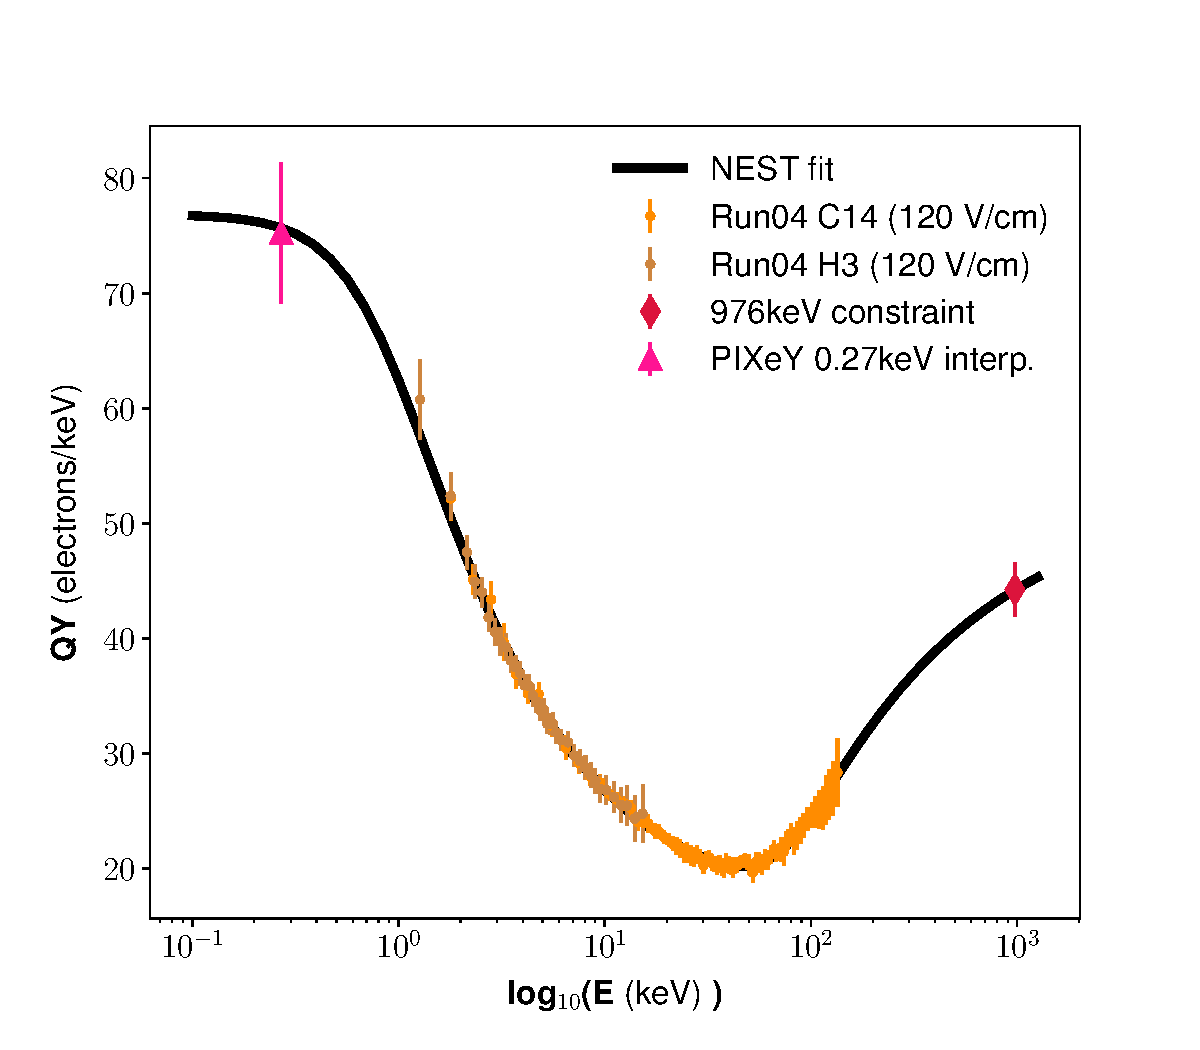
\includegraphics[width=\textwidth]{Figures/Yields_fit_old/NEST_fit_120Vcm_old.pdf}
  \caption{}
\end{subfigure}
\caption{Best fit $QY$ for ``gfdcm'' data in the 43, 53, 65, 80, 98, and 120 V/cm electric field bins. The orange points are the post-Run04 carbon-14 measurements, and the brown points are the post-Run04 tritium measurements. The other datasets are described in section \ref{sec:NESTbeta}.}
\label{fig:gfdcm_prelim_QY1}
\end{figure}

\begin{figure}[h!]
\centering
\begin{subfigure}{0.5\textwidth}
  \centering
  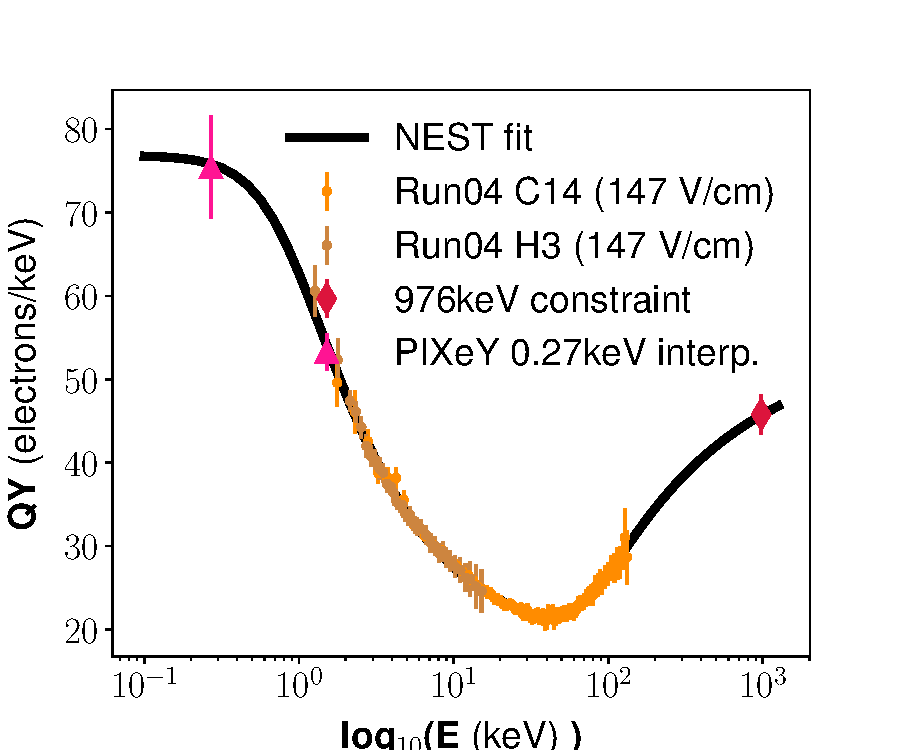
\includegraphics[width=\textwidth]{Figures/Yields_fit_old/NEST_fit_147Vcm_old.pdf}
  \caption{}
\end{subfigure}%
\begin{subfigure}{0.5\textwidth}
  \centering
  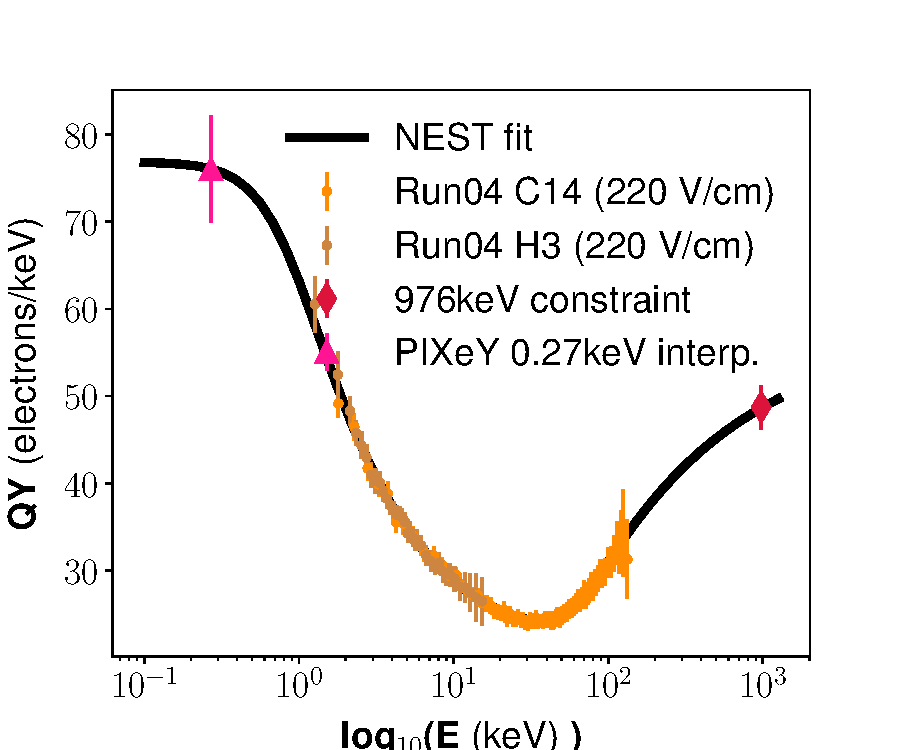
\includegraphics[width=\textwidth]{Figures/Yields_fit_old/NEST_fit_220Vcm_old.pdf}
  \caption{}
\end{subfigure}
\begin{subfigure}{0.5\textwidth}
  \centering
  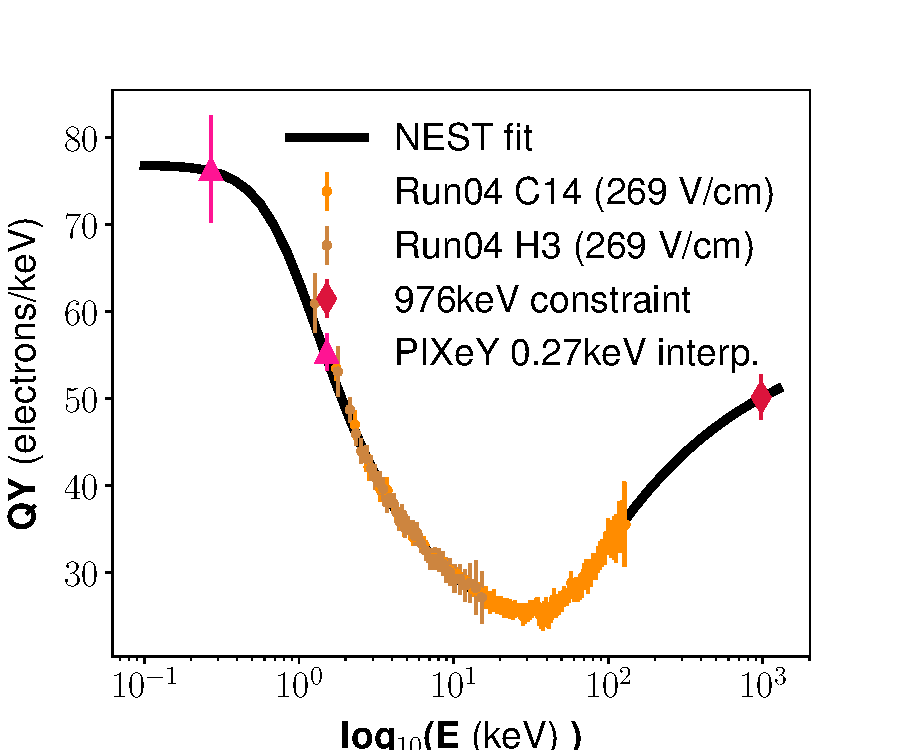
\includegraphics[width=\textwidth]{Figures/Yields_fit_old/NEST_fit_269Vcm_old.pdf}
  \caption{}
\end{subfigure}%
\begin{subfigure}{0.5\textwidth}
  \centering
  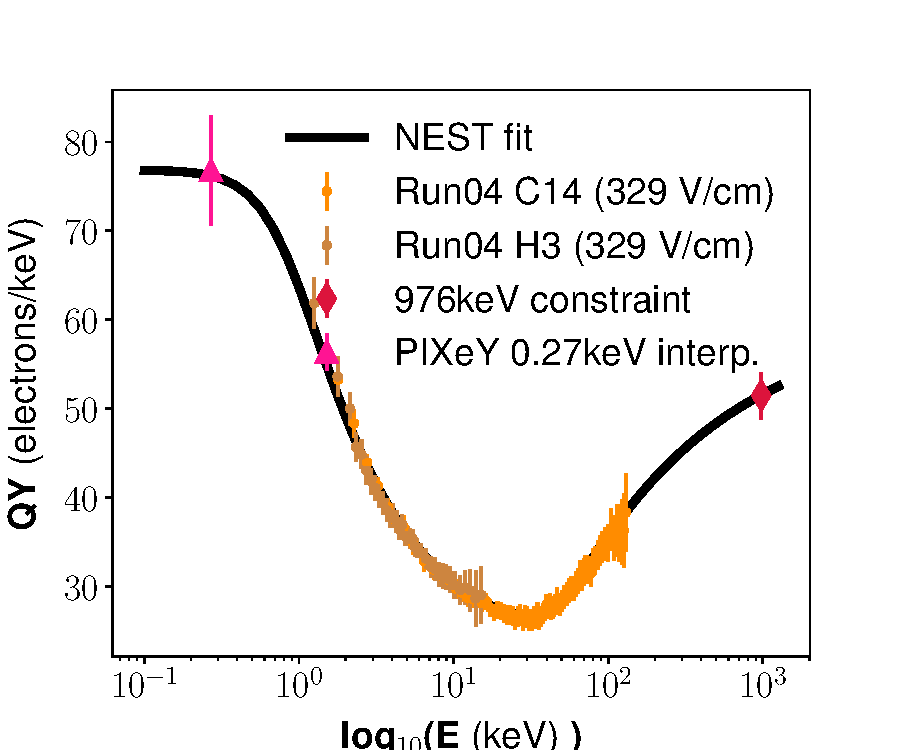
\includegraphics[width=\textwidth]{Figures/Yields_fit_old/NEST_fit_329Vcm_old.pdf}
  \caption{}
\end{subfigure}
\begin{subfigure}{0.5\textwidth}
  \centering
  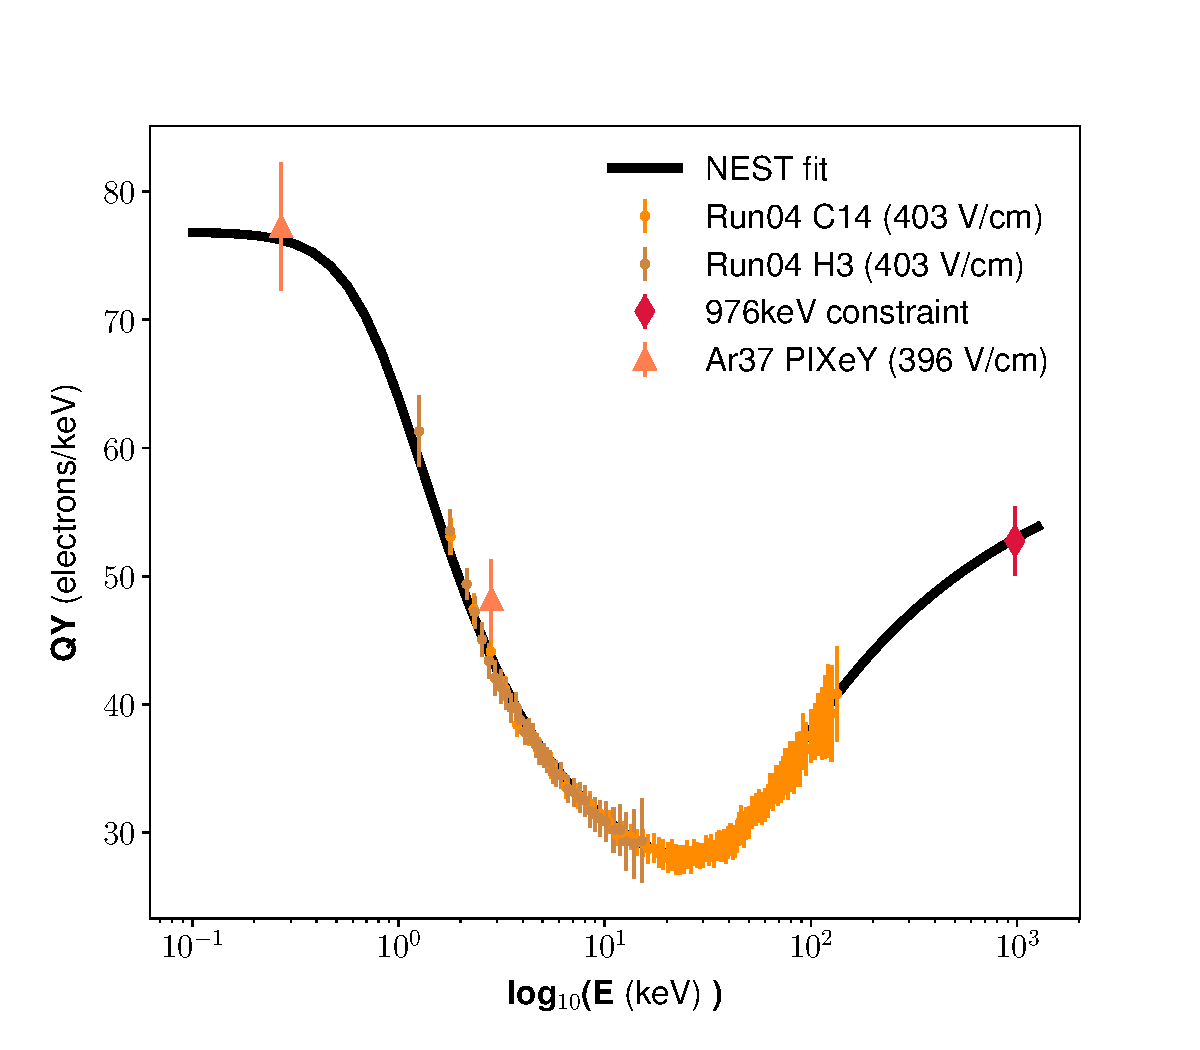
\includegraphics[width=\textwidth]{Figures/Yields_fit_old/NEST_fit_403Vcm_old.pdf}
  \caption{}
\end{subfigure}%
\begin{subfigure}{0.5\textwidth}
  \centering
  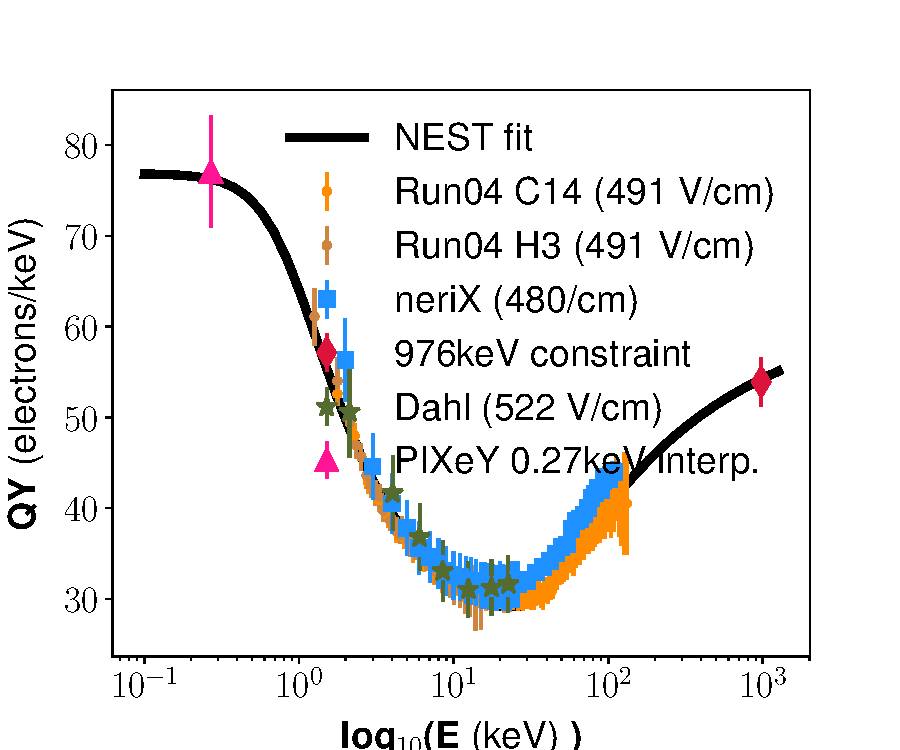
\includegraphics[width=\textwidth]{Figures/Yields_fit_old/NEST_fit_491Vcm_old.pdf}
  \caption{}
\end{subfigure}
\caption{Best fit $QY$ for ``gfdcm'' data in the 147, 220, 269, 329, 403, and 491 V/cm electric field bins. The orange points are the post-Run04 carbon-14 measurements, and the brown points are the post-Run04 tritium measurements. The other datasets are described in section \ref{sec:NESTbeta}.}
\label{fig:gfdcm_prelim_QY2}
\end{figure}

 
 
We also repeated these fits for the ``dcm'' data. We set $m_8=4.29$, $m_9= 0.334$, $m_2=77.3$, and $m_5=42.8$. The $m_3$ parameter was noisy throughout the bins, but had a general trend upward in electric field. Instead of holding it constant, we fit it to an exponential. We then proceeded to fit $m_1$, $m_7$, $m_4$, and $m_{10}$ to sigmoids as we did for the ``gfdcm'' data.  The results of these fits are shown in figures \ref{fig:dcm_prelim_params}, \ref{fig:dcm_prelim_QY180}, \ref{fig:dcm_prelim_QY1}, and \ref{fig:dcm_prelim_QY2}. We will use these fits when modeling both the ``dcm'' and ``z'' style corrections.
\begin{figure}[h!]
\centering
\begin{subfigure}{0.45\textwidth}
  \centering
  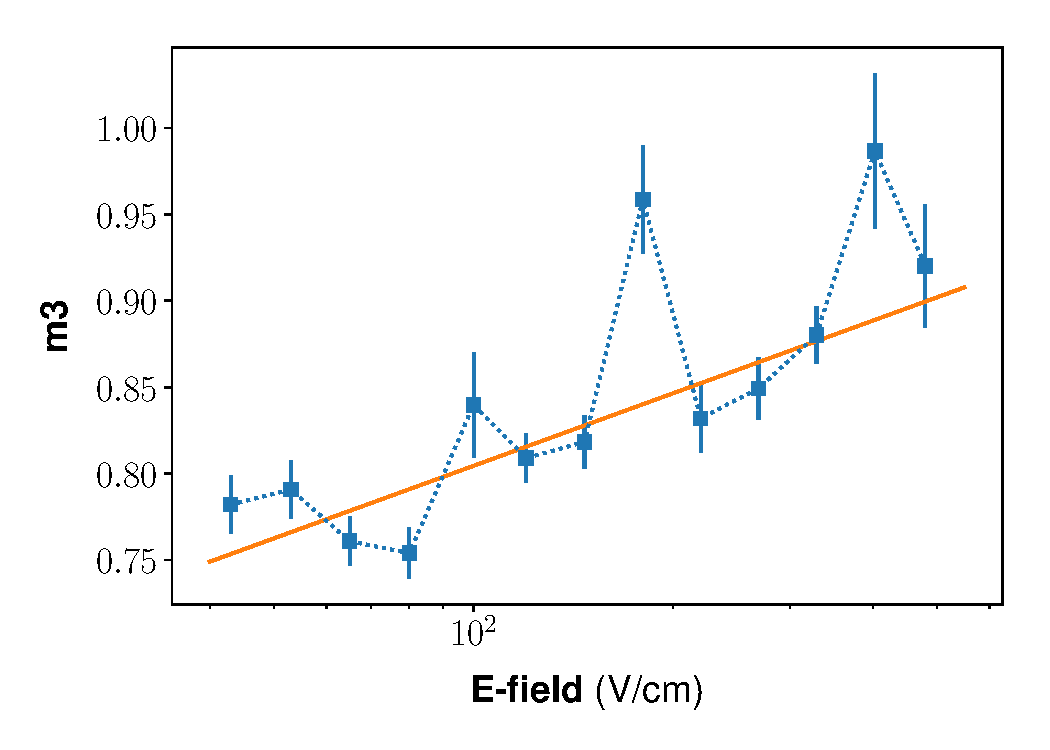
\includegraphics[width=\textwidth]{Figures/Yields_fit_old/NEST_m3_fit_old_dcm.pdf}
  \caption{}
\end{subfigure}%
\begin{subfigure}{0.45\textwidth}
  \centering
  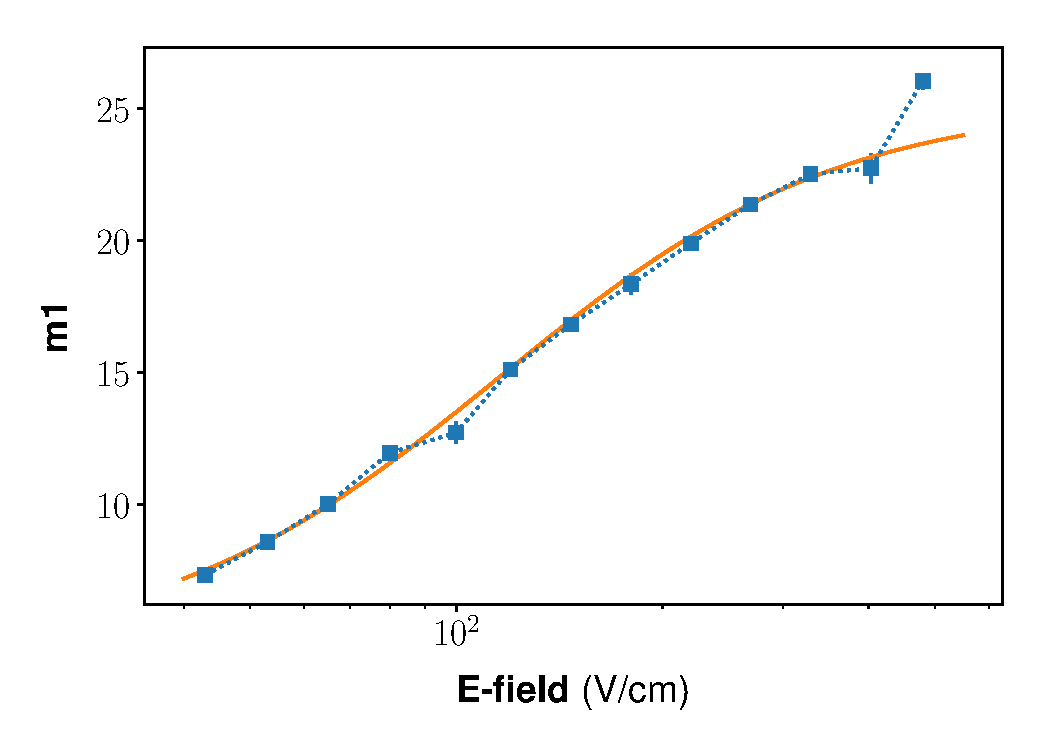
\includegraphics[width=\textwidth]{Figures/Yields_fit_old/NEST_m1_fit_old_dcm.pdf}
  \caption{}
\end{subfigure}
\begin{subfigure}{0.45\textwidth}
  \centering
  \includegraphics[width=\textwidth]{Figures/Yields_fit_old/NEST_m7_fit_old_dcm.pdf}
  \caption{}
\end{subfigure}%
\begin{subfigure}{0.45\textwidth}
  \centering
  \includegraphics[width=\textwidth]{Figures/Yields_fit_old/NEST_m4_fit_old_dcm.pdf}
  \caption{}
\end{subfigure}
\begin{subfigure}{0.45\textwidth}
  \centering
  \includegraphics[width=\textwidth]{Figures/Yields_fit_old/NEST_m10_fit_old_dcm.pdf}
  \caption{}
\end{subfigure}
\caption{Best fit $QY$ parameters as a function of electric field for the ``dcm'' style results. The parameters not shown in this figure are held constant in field at their error-weighted averages. The orange lines show sigmoid fits to the parameters as functions of electric field.}
\label{fig:dcm_prelim_params}
\end{figure}


\begin{figure}[h!]
  \centering
  \includegraphics[width=\textwidth]{Figures/Yields_fit_old/NEST_fit_180Vcm_old_dcm.pdf}
  \caption{Best fit $QY$ for ``dcm'' data in the 180 V/cm electric field bin. The orange points are the post-Run04 carbon-14 measurements, and the brown points are the post-Run04 tritium measurements. The datasets labeled ``Run03 H3'', ``Huang 2017'', and ``Pease 2017'' are all from LUX Run03 measurements. The blue squares are not included in the fit. The other datasets are described in section \ref{sec:NESTbeta}.}
  \label{fig:dcm_prelim_QY180}
\end{figure}


\begin{figure}[h!]
\centering
\begin{subfigure}{0.5\textwidth}
  \centering
  \includegraphics[width=\textwidth]{Figures/Yields_fit_old/NEST_fit_43Vcm_old_dcm.pdf}
  \caption{}
\end{subfigure}%
\begin{subfigure}{0.5\textwidth}
  \centering
  \includegraphics[width=\textwidth]{Figures/Yields_fit_old/NEST_fit_53Vcm_old_dcm.pdf}
  \caption{}
\end{subfigure}
\begin{subfigure}{0.5\textwidth}
  \centering
  \includegraphics[width=\textwidth]{Figures/Yields_fit_old/NEST_fit_65Vcm_old_dcm.pdf}
  \caption{}
\end{subfigure}%
\begin{subfigure}{0.5\textwidth}
  \centering
  \includegraphics[width=\textwidth]{Figures/Yields_fit_old/NEST_fit_80Vcm_old_dcm.pdf}
  \caption{}
\end{subfigure}
\begin{subfigure}{0.5\textwidth}
  \centering
  \includegraphics[width=\textwidth]{Figures/Yields_fit_old/NEST_fit_98Vcm_old_dcm.pdf}
  \caption{}
\end{subfigure}%
\begin{subfigure}{0.5\textwidth}
  \centering
  \includegraphics[width=\textwidth]{Figures/Yields_fit_old/NEST_fit_120Vcm_old_dcm.pdf}
  \caption{}
\end{subfigure}
\caption{Best fit $QY$ for ``gfdcm'' data in the 43, 53, 65, 80, 98, and 120 V/cm electric field bins. The orange points are the post-Run04 carbon-14 measurements, and the brown points are the post-Run04 tritium measurements. The other datasets are described in section \ref{sec:NESTbeta}.}
\label{fig:dcm_prelim_QY1}
\end{figure}

\begin{figure}[h!]
\centering
\begin{subfigure}{0.5\textwidth}
  \centering
  \includegraphics[width=\textwidth]{Figures/Yields_fit_old/NEST_fit_147Vcm_old_dcm.pdf}
  \caption{}
\end{subfigure}%
\begin{subfigure}{0.5\textwidth}
  \centering
  \includegraphics[width=\textwidth]{Figures/Yields_fit_old/NEST_fit_220Vcm_old_dcm.pdf}
  \caption{}
\end{subfigure}
\begin{subfigure}{0.5\textwidth}
  \centering
  \includegraphics[width=\textwidth]{Figures/Yields_fit_old/NEST_fit_269Vcm_old_dcm.pdf}
  \caption{}
\end{subfigure}%
\begin{subfigure}{0.5\textwidth}
  \centering
  \includegraphics[width=\textwidth]{Figures/Yields_fit_old/NEST_fit_329Vcm_old_dcm.pdf}
  \caption{}
\end{subfigure}
\begin{subfigure}{0.5\textwidth}
  \centering
  \includegraphics[width=\textwidth]{Figures/Yields_fit_old/NEST_fit_403Vcm_old_dcm.pdf}
  \caption{}
\end{subfigure}%
\begin{subfigure}{0.5\textwidth}
  \centering
  \includegraphics[width=\textwidth]{Figures/Yields_fit_old/NEST_fit_491Vcm_old_dcm.pdf}
  \caption{}
\end{subfigure}
\caption{Best fit $QY$ for ``dcm'' data in the 147, 220, 269, 329, 403, and 491 V/cm electric field bins. The orange points are the post-Run04 carbon-14 measurements, and the brown points are the post-Run04 tritium measurements. The other datasets are described in section \ref{sec:NESTbeta}.}
\label{fig:dcm_prelim_QY2}
\end{figure}

\clearpage
\section{Measurement of Recombination Fluctuations from $^{14}$C}
For an event with energy, $E$, and electric field, $\mathcal{E}$, is given by a certain number of electrons, $N_R$, will recombine with an ion. These electrons will be subtracted from the initial number of ions, $N_{i}$, and added to the number of excitons, resulting in the net number of electrons and photons produced by the event:
\begin{equation} 
\begin{split}
N_e=N_i-N_R \\
N_{\gamma}=\alpha N_e+N_R
\end{split}
\end{equation}
where the constant term $\alpha$  is the exciton to ion ratio. The expected value of $N_R$ will be given by:
\begin{equation}
\langle N_R \rangle = N_i\cdot P(E,\mathcal{E}),
\end{equation}
where $P(E,\mathcal{E})$ is the probability that an ionization electron will recombine. The expected charge yield for this event can then be written:
\begin{equation}
QY(E,\mathcal{E})=\frac{1}{W} \cdot \frac{1}{1+\alpha} \cdot \bigg(1-P_R(E,\mathcal{E})\bigg),
\end{equation}
where we have taken:
\begin{equation}
\Big(N_i\Big)/\Big(E\Big)=\Big( N_q\frac{1}{1+\alpha} \Big)\Big(N_q\cdot W\Big)= \frac{1}{W} \cdot \frac{1}{1+\alpha}
\end{equation}

Fluctuations in the recombination process, $\sigma_R$, will add to the fluctuations in detector resolution to give the total variance expected in the observed number of photons ($n_{\gamma}\equiv S1c/G1$) and electrons ($n_{e}\equiv S2c/G2$):
\begin{equation}\label{eq:detres_rec}
\begin{split}
\sigma_{\gamma}^2=\sigma_{R}^2+\sigma_{\gamma,det}^2\\[1em]
\sigma_{e}^2=\sigma_{R}^2+\sigma_{e,det}^2
\end{split}
\end{equation}
In the simplest model, where every ionization electron from an event has the same probability of recombining, the recombination fluctuations would be expected to follow a binomial trend:
\begin{equation}
\sigma_{binom}^2=nP(1-P)
\end{equation}
It has been observed, however, that $\sigma_R$ grows much more quickly than the $\sqrt{N_i}$ dependence expected for a binomial process. In fact, LUX Run03 data shows that the recombination fluctuations have an approximately linear dependence on the number of ions\cite{lux_tritium}:
\begin{equation}
\sigma_R=(0.073)\cdot N_i
\end{equation}



\subsection{Separating $\sigma_R$ from $\sigma_{det}$ in a Continuous Spectrum}
It is straightforward to calculate the recombination fluctuations from a mono-energetic line source without any prior knowledge of the detector resolution. In addition to equation \ref{eq:detres_rec} have also have: 
\begin{equation}
\sigma_E^2=W^2\left(\sigma_{\gamma,det}^2+\sigma_{e,det}^2\right),
\end{equation}
because the recombination process is orthogonal to energy. The recombination fluctuations can then be written in terms of the measurable quantities $\sigma_{S1}$, $\sigma_{S2}$, and $\sigma_{E}$:
\begin{equation}\label{eq:sigrline}
\sigma_{R,line}=\frac{1}{2}\left(\sigma_{\gamma}+\sigma_{S2}-\frac{\sigma_{E}}{W}\right)
\end{equation}
However, just as in the case of charge and light yields measurements, the measurement of $\sigma_R$ by dividing a continuous spectrum into energy bins is significantly more complex than using all of the events from a mono-energetic source. 

In a continuous spectrum such as tritium and carbon-14, we do not have immediate access to any of the measurables that go into the calculation of \ref{eq:sigrline}. The energy resolution is convolved with the spectral shape making a direct measurement nearly impossible. As we found in section \ref{sec:desmearing}, $\sigma_{\gamma,det}$, $\sigma_{e,det}$, and $\sigma_{R}$ all smear the measured band of ($n_{e}$,$n_{\gamma}$) in nontrivial ways, making it difficult to reconstruct how a measurement in a reconstructed energy bin corresponds to the underlying physical process. We again turn to the method laid out in \cite{attila} for guidance, although the addition of the pathological S2 tails may again make this method largely ineffective for the post-Run04 data. 

\begin{figure}[h!]
\centering
\begin{subfigure}{0.5\textwidth}
  \centering
  \includegraphics[width=\textwidth]{Figures/Attila_chi_reconly.pdf}
  \caption{}
\end{subfigure}%
\begin{subfigure}{0.5\textwidth}
  \centering
  \includegraphics[width=\textwidth]{Figures/Attila_chi_norec.pdf}
  \caption{}
\end{subfigure}
\caption{The left plot (a) shows the binning of a toy spectrum with recombination fluctuations, but no detector fluctuations. All of the events fall within the reconstructed energy bin, so the variance of events within the bin is equal to the total variance of the population. The right plot (b) shows the binning of a toy spectrum with no recombination fluctuations, but with detector fluctuations. In this case, the total photon width, $\sigma_{\gamma}=172.5$ is much greater than the deviation within the energy bin, $\chi_{\gamma}=52.6$. Meanwhile the total deviation in the electron spectrum $\sigma_{e}=50.7$ is about equal to the deviation within the bin, $\chi_e=50.0$. The discrepancy in $\chi_{\gamma}$ and $\chi_e$ is due to the finite width of the energy bin. Figures taken from \cite{attila}.}
\label{fig:attila_chi}
\end{figure}
We examine the behavior of the S1 and S2 spectra within an energy slice. We will define the total variance of the S1 and S2 populations within this slice to be:
\begin{equation}
\chi_{tot}^2\equiv  \frac{\sigma_{S1,slice}^2}{G1^2} = \frac{\sigma_{S2,slice}^2}{G2^2}
\end{equation}
The events in the bin will all have about the same reconstructed energy, so an event with $n_{e}=\langle n_{e} \rangle +N_R$ will have a corresponding $n_{\gamma}\approx \langle n_{\gamma} \rangle -N_R$. Therefore, the variance of the $n_{\gamma}$ spectrum will be equal to that of the $n_{e}$ spectrum within the bin. 

The recombination fluctuations do not affect an event's reconstructed energy, so in a detector with infinite detector resolution, the variance of events within an energy bin will be equal to the recombination variance of events at that energy:
\begin{equation} 
\chi_{R}=\sigma_{R}
\end{equation}
In the case of a detector with finite detector resolution but no recombination fluctuations, the relation between $\chi_{det}$, $\sigma_{e,det}$, and $\sigma_{\gamma,det}$ is significantly more complicated. 

For example, consider figure \ref{fig:attila_chi} which shows a spectrum from a simulated krypton-83m source. The left plot has $\sigma_R=90.3$ and $\sigma_{e,det}=\sigma_{\gamma,det}=0$. In this case, all of the events fall within the reconstructed energy bin, so the variance of events within the bin is equal to the total variance of the population. In the right plot we have $\sigma_R=0$, $\sigma_{e,det}=50.7$, and $\sigma_{\gamma,det}=172.5$. The width of the full photon population, $\sigma_{\gamma}=172.5$ is much greater than the deviation within the energy bin, $\chi_{\gamma}=52.6$. Meanwhile the total deviation in the electron spectrum $\sigma_{e}=50.7$ is about equal to the deviation within the bin, $\chi_e=50.0$. Conceptually, we see this is because the deviation of events within the energy slice is limited by the deviation in the number of electrons. An event with a larger upward fluctuation in $n_{\gamma}$ must have an equally large fluctuation downward in $n_{e}$ in order to pass the energy cut, but here we have $\sigma_{\gamma,det} \approx 3 \cdot \sigma_{e,det}$ so a 1-sigma fluctuation in $n_{\gamma}$ requires a 3-sigma fluctuation in $n_{e}$ in order to be selected by the energy bin. Meanwhile, a 1-sigma fluctuation in $n_{e}$ would require a 0.3-sigma fluctuation in $n_{\gamma}$ to be selected, so $\chi_{e,det}$ is only slightly narrower than $\sigma_{e,det}$. We also note a small discrepancy in $\chi_{\gamma}$ and $\chi_e$; this is due to the finite width of the energy bin\cite{attila}. 

\begin{figure}[h!]
  \centering
  \includegraphics[width=\textwidth]{Figures/toysigR_ellipse_graphic.pdf}
\caption{Calculation of $\chi_{det}$ using a rotated error ellipse. We used typical LUX parameters for an 80 keV decay. We set $QY$ = 25 electrons per keV, $QY$ = 48 photons per keV, $\sigma_{\gamma,det}$ = 216.2 photons, and $\sigma_{\gamma,det}$= 33.1 electrons. The light green line shows the trend-line of the ($n_e,n_{\gamma}$) band. The heavy green line shows the 1-sigma error band. The dashed black line is the 80 keV line of constant energy. The solid black lines indicate $\chi_{det}$; the size of the fluctuations of $n_e$ and $n_{\gamma}$ along the line of constant energy. }
\label{fig:errorellipse}
\end{figure}
To obtain a better quantitative understanding of $\chi_{det}$, Dobi analyzed small fluctuations along lines of constant energy using $E/W\equiv n_q=n_e+n_{\gamma}$; first holding $n_{\gamma}$ and allowing for fluctuations in $n_e$, and then holding $n_e$ constant, allowing for fluctuations in $n_{\gamma}$\cite{attila}:
\begin{equation}\label{eq:smallvar}
\begin{split}
\delta n_{q,\bot}&=\frac{\partial n_{\gamma}}{\partial n_{q}}\delta n_{q} \Big| _{n_{\gamma}}+\frac{\partial n_{e}}{\partial n_{q}}\delta n_{q} \Big| _{n_{e}}\\
&=\frac{\partial n_{\gamma}}{\partial n_{q}}\delta n_{e}+\frac{\partial n_{e}}{\partial n_{q}}\delta n_{\gamma}
\end{split}
\end{equation}
We square equation \ref{eq:smallvar}, dropping the cross-terms because $\sigma_{e,det}$ and $\sigma_{\gamma,det}$ are uncorrelated. This gives the following expression for $\chi_{det}$:
\begin{equation}\label{eq:chidet}
\chi_{det}^2=\left(\frac{\partial n_{\gamma}}{\partial n_{q}}\right)^2\sigma_{e,det}^2+\left(\frac{\partial n_{e}}{\partial n_{q}}\right)^2\sigma_{\gamma,det}^2
\end{equation}
In the case of a line source with, $\frac{\partial n_{\gamma}}{\partial n_{q}}$ would be the slope of the major axis of the error ellipse in ($n_q,n_{\gamma}$) space:
\begin{equation}
\frac{\partial n_{\gamma}}{\partial n_{q}}= \frac{\sigma_{\gamma,det}^2}{\sigma_{\gamma,det}^2+\sigma_{e,det}^2}
\end{equation}
Similarly, the slope for electrons would be:
\begin{equation}
\frac{\partial n_{e}}{\partial n_{q}}=1-\frac{\partial n_{\gamma}}{\partial n_{q}}= \frac{\sigma_{e,det}^2}{\sigma_{\gamma,det}^2+\sigma_{e,det}^2}
\end{equation}
In the case of a continuous spectrum, the slopes $M_{\gamma}=\frac{\partial n_{\gamma}}{\partial n_{q}}$ and $M_{e}=\frac{\partial n_{e}}{\partial n_{q}}$ could be approximated by $LY\cdot W$ and $QY\cdot W$, respectively.

Equation \ref{eq:chidet} can also be derived by rotating the error ellipse by the angle of the central trend-line of the ($n_e,n_{\gamma}$) band, as shown in figure \ref{fig:errorellipse}. For this figure, we used typical LUX parameters for an 80 keV decay. We set $QY$ = 25 electrons per keV, $QY$ = 48 photons per keV, $\sigma_{\gamma,det}$ = 216.2 photons, and $\sigma_{\gamma,det}$= 33.1 electrons. The orthogonal height of the error ellipse rotated by $\theta=\text{arctan}(M_{\gamma}/M_{e})$, which is equivalent to the band width ($\sigma_B$), is given by:
\begin{equation}
\sigma_B=\sqrt{\Big(\sigma_{e,det}\sin(\theta)\Big)^2+\Big(\sigma_{\gamma,det}\cos(\theta)\Big)^2}
\end{equation}
We find $\chi_{det}$ by calculating the point at which the 80 keV constant energy line intersects the ``band mean + 1$\sigma$'' line and then project onto the x and y axes. This yields:
\begin{equation}
\begin{split}
\chi_{det}&=\frac{\sigma_B}{\sin(\theta)+\cos(\theta)}\\[1em]
&=\frac{\sigma_B\cdot \sqrt{M_e^2+M_{\gamma}^2}}{M_e+(1-M_e)}\\[1em]
&=\sqrt{\sigma_{e,det}^2M_{\gamma}^2+\sigma_{\gamma,det}^2M_{e}^2},
\end{split}
\end{equation}
which reproduces the results from equation \ref{eq:chidet}.

\subsection{Recombination Fluctuations with S2 Tails}
The procedure we have laid out for extracting recombination fluctuations from a continuous beta spectrum was used with success on the LUX Run03 tritium data\cite{lux_tritium}. However, we again must contend with the addition of the pathological S2 tails. To investigate how $\chi_{det}$ will be affected by the tails, we generate two toy carbon-14 spectra of ($n_{e}$,$n_{\gamma}$); one with tails and one without. We use the yields model measured in section \ref{sec:qyprelim} to determine the central values of $n_e$ and $n_{\gamma}$ for each event. We then apply recombination fluctuations based on the model in \cite{lux_tritium}, $\sigma_R=0.0734\cdot N_i$. For the detector resolution, we take $\sigma_{e,det}=0.74\sqrt{n_e}$ and $\sigma_{\gamma,det}=3.5\sqrt{n_{\gamma}}$. For the pathological tails, we follow the model from section \ref{sec:s2tails} where each S2 has a probability $R=0.45$ of having tail area added to it, and the tail area is drawn from an exponential distribution with mean $\mu=S2\cdot b=S2 \cdot 0.16$. The variance in the tail area will contain a contribution from the exponential distribution, as well as a contribution from a binomial process with probability $R$. The variance of an exponential distribution is $\mu^2$, so we will model the variance in the tail area using:
\begin{equation}
\begin{split}
\sigma_{tail}^2&= R^2(S2\cdot b)^2+(S2\cdot b)^2\cdot R(1-R)\\
&=R(S2\cdot b)^2
\end{split}
\end{equation}
For each of the models, with tails and without tails, we generate an additional spectrum that does not include recombination fluctuations.
\afterpage{%
\begin{figure}[p]%
\centering
\begin{subfigure}{0.5\textwidth}
  \centering
  \includegraphics[width=\textwidth]{Figures/toysigR_heatmap_notail.pdf}
  \caption{}
\end{subfigure}%
\begin{subfigure}{0.5\textwidth}
  \centering
  \includegraphics[width=\textwidth]{Figures/toysigR_heatmap_wtail.pdf}
  \caption{}
\end{subfigure}
\begin{subfigure}{0.5\textwidth}
  \centering
  \includegraphics[width=\textwidth]{Figures/toysigR_notail.pdf}
  \caption{}
\end{subfigure}%
\begin{subfigure}{0.5\textwidth}
  \centering
  \includegraphics[width=\textwidth]{Figures/toysigR_wtail.pdf}
  \caption{}
\end{subfigure}
\caption{Models of recombination fluctuations. The left plots, (a) and (c), show a model which does not include S2 tails, while the model shown by (b) and (d) do include our S2 tail model. $\sigma_{R}$ shows the expected recombination fluctuations for the average energy of events in each bin. $\chi_{det}$ shows the expected band width due to $\sigma_{\gamma,det}$ and $\sigma_{e,det}$; it is calculated using equation \ref{eq:chidet}, with $\frac{\partial n_e}{\partial n_{q}}=QY/73$ and $\frac{\partial n_{\gamma}}{\partial n_{q}}=LY/73$. $\chi_{tail}$ is the expected added contribution due to the S2 tails. The two lines $\chi_{tot}$ and $\chi_{noR}$ are the measured band widths for the model with $\sigma_R$ and without $\sigma_R$, respectively. Finally, we have defined $|\Delta\chi^2|= | \chi_{tot}^2-(\chi_{noR}^2+\sigma_R^2)|$.}
\label{fig:toysigr}
\end{figure}
    \clearpage
}

The results of these models are shown in figure \ref{fig:toysigr}. The left-hand plots show the model with no tails, while the right-hand plot shows the model with tails. In these plots, $\sigma_{R}$ shows the expected recombination fluctuations for the average energy of events in each bin. $\chi_{det}$ shows the expected band width due to $\sigma_{\gamma,det}$ and $\sigma_{e,det}$; it is calculated using equation \ref{eq:chidet}, with $\frac{\partial n_e}{\partial n_{q}}=QY/73$ and $\frac{\partial n_{\gamma}}{\partial n_{q}}=LY/73$. $\chi_{tail}$ is the expected added contribution due to the S2 tails. The two lines $\chi_{tot}$ and $\chi_{noR}$ are the measured band widths for the model with $\sigma_R$ and without $\sigma_R$, respectively. Finally, we have defined $|\Delta\chi^2|= | \chi_{tot}^2-(\chi_{noR}^2+\sigma_R^2)|$ to test the assumptions that went into our method for extracting recombination fluctuations. This value will give us a hard limit as to how well we can measure recombination fluctuations using this method.

If our method is valid, the ``$\chi_{det}^2$'' and ``$\chi_{det}^2+\chi_{tail}^2$'' will lie on top of their respective ``$\chi_{noR}^2$'' lines and $|\Delta\chi^2|$ should be close to zero. We find that this is the case for the model with no S2 tails. The ``$\chi_{det}^2$'' line closely follows the measured ``$\chi_{noR}$'' line across the entire energy range. Additionally, $|\Delta\chi^2|$ remains small at all energies; it is $<$ 10\% of $\chi_{tot}$ at all energies, and is $<$ about 1\% of $\sigma_R$ above keV 20.

As it was with the yields measurements, the Run03 method for extracting recombination fluctuations breaks down when S2 tails are added. Both of our tests for validity fail for our tailed model. The ``$\chi_{det}^2+\chi_{tail}^2$'' line is clearly not predicting the trend of the ``$\chi_{noR}$'' line, and $|\Delta\chi^2|$ is on the order of 10\% of $\sigma_{R}$ across the entire energy range. The ability to account for detector resolution is even more important in the tailed model because the measured $\chi_{noR}^2$ has increased by about an order of magnitude over what it was for the un-tailed model. For these reasons, we will abandon this method of calculating recombination fluctuations and will again perform the measurement numerically. 


\subsection{Modelling $^{14}$C Recombination Fluctuations in libNEST}\label{sec:sigrupdate}
The S2 tails interact with the recombination fluctuations and detector resolution in a non-trivial way, making our previous method of measuring recombination fluctuations from a beta spectrum invalid. We no longer have access to the value of $\sigma_R$ in an individual energy bin. Instead we use results from prior experiments to motivate a functional form of $\sigma_R(E,\mathcal{E})$, inputting that model into the libNEST code, and optimizing its parameters. 

As mentioned previously, it was found that the recombination fluctuations in the LUX Run03 tritium data is consistent with\cite{lux_tritium}:
\begin{equation}
\sigma_R=0.0734 \cdot N_i
\end{equation}
This model has been modified in several subsequent papers, but the underlying trend remains the same.


There is a set of measurements from the Xenon10 experiment which studied the fluctuations in a cobalt-57 deposit in liquid xenon at various electric fields. The results from this experiment, which are published in Eric Dahl's thesis \cite{dahl}, suggest that a pure linear trend in $N_i$ is not sufficient to characterize all of the features of $\sigma_R$ as a function of energy and electric-field. In the left panel of figure \ref{fig:sigR_wRun03pDahl}, we have displayed the results from this experiment, which were digitized from \cite{dahl}. The blue markers indicate measurements of $\sigma_R$ at various electric fields; $^{57}$Co is a mono-energetic source, so $N_i$ will be the same for each of these measurements. The Run03 tritium model, displayed as the black line in figure \ref{fig:sigR_wRun03pDahl}, predicts that $\sigma_R$ would be constant in field, but we see that the $^{57}$Co measurements follow roughly quadratic shape when plotted as a function of $y\equiv n_e/n_q$ with a peak near $y=0.5$. The prediction from Run03 tritium is in agreement with the peak value of $\sigma_R$ as measured by $^{57}$Co.
\begin{figure}[!h]
\centering
  \includegraphics[width=\textwidth]{Figures/sigR_wRun03pDahl_gfdcm.pdf}
\caption{Comparison of the linear Run03 model of $\sigma_R$ (black line) to the updated model (blue line). The points labeled ``Dahl thesis'' show measurements of $^{57}$Co at varying fields, and are digitized from \cite{dahl}. The black ``x's'' show data from LUX Run03. The low energy points are from tritium, and the high energy points are primarily $^{137}$Cs. These points were digitized from \cite{lux_tritium}. The new model does a significantly better job at reproducing the shape of both the cobalt-57 data and the LUX Run03 data. }
\label{fig:sigR_wRun03pDahl}
\end{figure}

With this in mind, we propose the following expression for $\sigma_R$:
\begin{equation}\label{eq:sigrmod_gen}
\sigma_{R}(E,\mathcal{E})^2=P_{R}(1-P_{R})\cdot N_i +F_{R}(\frac{n_e}{n_q})N_i^2
\end{equation}
This is actually very similar to the Run03 tritium model, with the primary difference being that $F_R$ here is a function of the electron-fraction, $y$, whereas in the Run03 model $F_R=0.0734^2$ was a constant. We also force $\sigma_R^2$ to be no less than the variance of a binomial process by explicitly adding the binomial term $P_{R}(1-P_{R})\cdot N_i$ to equation \ref{eq:sigrmod_gen}.

The question remains as to what the functional form of $F_{R}(\frac{n_e}{n_q})$ should be. We first tested a simple quadratic against the carbon-14 data, but found it fell too quickly toward low $y$ and was not able model data from all of the electric field bins simultaneously. We instead switched to a Gaussian and found that this model did a fair job at capturing the band width of the carbon-14 data in all of the field bins. Equation \ref{eq:sigrmod_gen} then becomes:
\begin{equation}\label{eq:sigrmod}
\sigma_{R}(E,\mathcal{E})^2=P_{R}(1-P_{R})\cdot N_i +\left(F_0\exp \left(\frac{-(n_e/n_q-F_1)^2}{2F_2^2}\right)\right)^2N_i^2,
\end{equation}
where $F_0$, $F_1$ and $F_2$ will be constant fitting parameters.
\begin{figure}[h!]
\centering
  \includegraphics[width=\textwidth]{Figures/sigR_fit_gfdcm.pdf}
\caption{Fitting results for the updated model of the recombination fluctuations.}
\label{fig:sigrfit}
\end{figure}

We find $F_0$, $F_1$, and $F_2$ by folding equation \ref{eq:sigrmod} into the libNEST code and generating a simulated carbon-14 spectrum. We then bin in energy and calculate the width of the S1 and S2 spectra in each bin. The width of the bands in a bin ($\chi_{S1(S2)}$) is calculated by fitting a Gaussian to its spectrum; we make a histogram of the binned data, apply a selection cut on the histogram centers, and then fit to to selected histogram values. The selection cut for S2 is -2 to 1 standard deviations from the mean, and for S1 is -1 to 2 standard deviations from the mean. In each energy bin, and for both data and simulation, we will then have a measurement of the width of the S1 and S2 bands along with values for the fitting uncertainty. We then take the average chi-squared difference between the data and simulation bands as the reduced chi-squared value for each band. We repeat this for all of the electric field bins, for both tritium and carbon-14 data. We sum the resulting set of reduced chi-squared values to give us a goodness-of-fit parameter ($GoF_{Run04}$) for a given set of ($F_0$, $F_1$, $F_2$):
\begin{equation}
\begin{split}
()_{S1}=&\sum_{\mathcal{E}_i}\left\langle \frac{\bigg(\text{S1 width})_{i,dat}-(\text{S1 width})_{i,sim}\bigg)^2}{(\text{S2 fitting error})_{i,dat}^2+(\text{S2 fitting error})_{i,dat}^2}\right\rangle \\[1em]
GoF_{Run04}=&GoF_{S1,^{14}C}+GoF_{S2,^{14}C}+GoF_{S1,^3H}+GoF_{S2,^3H}
\end{split}
\end{equation}

We also want to include results from the previous experiments in our fit, so we calculate a goodness of fit parameter ($GoF_{Dahl}$) for the data shown in figure \ref{fig:sigR_wRun03pDahl}. We define $GoF_{Dahl}$ to be equal to the chi-squared error error between the $^{57}$Co points and our test model. We find that our data is not in agreement with ``Dahl Thesis'' data at low values of $y$, so we only include points above $y=0.4$ in our calculation of $GoF_{Dahl}$. 

We then define a loss function:
\begin{equation}
loss=\log_{10}(GoF_{Run04}+w_{Dahl}\cdot GoF_{Dahl})
\end{equation}
The weight ($w-{Dahl}$) applied to $GoF_{Dahl}$ was tuned until it is a heavy enough that the best fit model captures the high-$y$ points in the cobalt-57 dataset but not so heavy that the Run04 data is overpowered in the low-$y$ region. We selected a weight factor of 5, but the fitting result is insensitive to changes in $w_{Dahl}$ of up to a factor of 2.

We will take the set of ($F_0$, $F_1$, $F_2$) which minimizes this loss function to be our best fit parameters. To find this minimum, we set up a 3-D grid in ($F_0$, $F_1$, $F_2$) and evaluate the loss function at the center of each box in the grid. We take the uncertainty on $F_0$ to be the width of a grid spacing, as is shown in figure \ref{fig:sigrfit}. The uncertainties on $F_1$ and $F_2$ are taken to be 3 and 2 grid spacings, respectively, because the loss function is not as steep as it is for $F_0$, so random fluctuations can beat the slope and the trend outward from the ($F_1,F_2$) optimum is not entirely monotonic. There is some subjectivity in our choice of $w_{Dahl}$. To characterize the uncertainty in our parameters added by this subjectivity, we vary $w_{Dahl}$ up and down by a factor of 5 to see how the best fit values are affected. We find that when $w_{Dahl}=1$ and when $w_{Dahl}=25$, all of the best fit parameters deviate by exactly the previously stated error. We will therefore multiply these error by $\sqrt{2}$.

Using ``gfdcm'' data we find our best fit parameters are:
\begin{equation}\label{eq:sigrbestfit}
\begin{split}
F_0=0.075 \pm 0.005\\
F_1=0.4975 \pm 0.02\\
F_2=0.206 \pm 0.02
\end{split}
\end{equation}
We find that the results for ``z'' and ``dcm'' data are identical. The best-fit model is shown in figures \ref{fig:sigR_fieldvar_gfdcm} and \ref{fig:sigR_fieldvar_dcm}. We find that this model is much improved over the simple linear model, and that it does a decent job at characterizing the width of both the carbon-14 S1 and S2 bands in all of the field bins. The new libNEST model does tend to overestimate the width below about 30 keV, but it is not clear where the model is failing. It is possible, for instance, that our model of the S2 tails does not work in this region.

\begin{figure}[h!]
\centering
  \includegraphics[width=\textwidth]{Figures/sigR_fieldvar_gfdcm.pdf}
\caption{Comparison of the libNEST model of S1 and S2 widths, using the updated recombination model to the widths as measured in the ``gfdcm'' data. }
\label{fig:sigR_fieldvar_gfdcm}
\end{figure}
\begin{figure}[h!]
\centering
  \includegraphics[width=\textwidth]{Figures/sigR_fieldvar_dcm.pdf}
\caption{Comparison of the libNEST model of S1 and S2 widths, using the updated recombination model to the widths as measured in the ``dcm'' data. }
\label{fig:sigR_fieldvar_dcm}
\end{figure}

\clearpage

\section{Results from Post-Run04 $^{14}$C and $^{3}$H Calibrations}\label{sec:finalresults}
\subsection{Yields and Recombination}
We now have all of the ingredients we need to measure the charge and light yields using the post-Run4 carbon-14 and tritium data. The preliminary measurements of the charge yield obtained in section \ref{sec:qyprelim} are combined with the new model for recombination fluctuations derived in section \ref{sec:sigrupdate}, and both are input into the libNEST code. We then reapply the Metropolis fits for the S2 tail parameter fits from section \ref{sec:s2tails} in order to account for any changes due to the updated parameters. The yields for gamma-type events are known to be different from beta-yields, so we use the existing set of yields when fitting the $^{131m}$Xe peak. The results of these fits, which are shown in table \ref{tab:s2bestfit_new}, are consistent with those found previously.
\begin{table}[h!]
\centering
    \begin{tabular}{ c | c | c | c | c | c | c }
    \hline
    Correction & b$_{tail}$ & $\pm$ & P$_{tail}$ & $\pm$  & G2$_{true}$ & $\pm$ \\
    \hline \hline
    z & 0.112 & 0.003 & 0.73 & 0.02 & 17.61 & 0.06\\
    \hline
    dcm & 0.116 & 0.004 & 0.62 & 0.02 & 17.36 & 0.05 \\
    \hline
    gfdcm & 0.110 & 0.004 & 0.52 & 0.02 & 16.04 & 0.04 \\
    \hline
    \end{tabular}
    \caption{Updated best fit results for the S2 tail model using the preliminary yields measurements and new $\sigma_R$ model.}
    \label{tab:s2bestfit_new}
\end{table}

The addition of the newly fit tail parameters gives us a fully armed and operational model which we input into the libNEST infrastructure in order to recalculate the tritium and carbon-14 spectra. The newly simulated spectra are used to un-smear the $E_{rec}$, $n_{\gamma}$, and $n_e$ using the method laid out in section \ref{sec:desmearprelim}. We thereby obtain final values for $\langle E_{true} \rangle_{ij}$, $\langle N_{\gamma} \rangle_{ij}$ and $\langle N_{e} \rangle_{ij}$. The ``$i$'' refers to the reconstructed energy bins described in section  \ref{sec:desmearprelim}, and the ``$j$'' subscripts refer to the electric field bins laid out in section \ref{sec:fieldbins}.

In order to calculate the light yield ($LY$), charge yield ($QY$), and recombination fraction ($r$), we define a new parameter which will be equal to the ratio of photons to electrons:
\begin{equation}
\rho \equiv \frac{N_{\gamma}}{N_e}=\frac{LY}{QY}
\end{equation}
Using $1/W=LY+QY$, the three parameters of interest can then be calculated:
\begin{equation}\label{eq:translate_rho}
\begin{split}
LY&=\frac{1}{W}\frac{1}{1+\rho}\\[1em]
QY&=\frac{1}{W}\frac{\rho}{1+\rho}\\[1em]
r&=\frac{\rho-\alpha}{1+\rho}
\end{split}
\end{equation}

The energy bins we used for carbon-14 are identical to those described in table \ref{tab:ebins_c14}. However, we found that the lowest energy binning was not fine enough for the tritium data. The systematic error due to binning was by far the dominant error in these bins. For the final measurements, we updated our binning as described in table \ref{tab:ebins_h3_new}.
\begin{table}[h!]
\centering
    \begin{tabular}{ c || c | c | c | c  }
    \hline
    Energy Range (keV) & 1-6  & 6-10 & 10-14 & 14-18\\
    \hline
    Bin Width (keV)         &  0.2      &  0.5         & 1           & 2 \\
    \hline
    \end{tabular}
    \caption{Tritium reconstructed energy bin widths and their associated energy ranges for the final measurements of $\langle \rho \rangle$.}
    \label{tab:ebins_h3_new}
\end{table}

For our set of electric field and energy bins, we use our measured $\langle N_{\gamma} \rangle_{ij}$ and $\langle N_{\gamma} \rangle_{ij}$ to calculate $\langle \rho \rangle_{ij}$. The measured values of $\langle E_{true} \rangle$ and $\langle \rho \rangle$ values are reported in appendix \ref{sec:results_tables}. The systematic errors shown for $\langle \rho \rangle$ include the de-smearing error as well as the uncertainty in G1 and G2. The best-fit values for G1 and G2 have non-negligible correlation, so the cross-term is included in the error propagation. We also include a 4.3\% systematic uncertainty on $\langle N_{\gamma} \rangle$, which comes from the rms offset from the Doke plot line shown in figure \ref{fig:dt_doke_plot} and quantifies any remaining position dependence in G1 and G2 that our efficiency corrections failed to remove. The uncertainties due to smearing and efficiency corrections are comparable in most of the energy bins and are the dominant systematic error. Near the endpoints of the spectra, the smearing error becomes dominant.

The uncertainties shown for $\langle E_{true} \rangle$ include the smearing error as well as the error due to finite bin width. We take the uncertainty due to a bin width of $\Delta E$ from the variance of a uniform distribution:
\begin{equation}
\sigma_{E,bin}^2=\frac{\Delta E^2}{12}
\end{equation}
\begin{figure}[!h]
\centering
\begin{subfigure}{0.5\linewidth}
\centering
  \includegraphics[width=\linewidth]{Figures/rho_ratio_final.pdf}
\caption{}
\end{subfigure}%
\begin{subfigure}{0.5\linewidth}
\centering
  \includegraphics[width=\linewidth]{Figures/QY_ratio_final.pdf}
\caption{}
\end{subfigure}
\caption{Ratio between the results for $\langle \rho \rangle$ (a) and QY (b) for the various corrections methods. The red lines indicate ``z''/``gfdcm'' data, and the black lines indicated ``dcm''/``gfdcm'' data. The light dotted lines indicate ratios in individual field-bins for both carbon-14 and tritium. The dark dashed lines show the average of tritium datasets over all of the field bins, and the solid lines show the average of carbon-14 datasets. }
\label{fig:rho_ratio}
\end{figure}

These measurements are also shown in figures \ref{fig:C14_rho_final} and \ref{fig:H3_rho_final}. In these plots, the error-bars represent the systematic and statistical uncertainties are added together in quadrature. We can see here that there is some discrepancy between the various corrections-methods defined in section \ref{sec:corrections}. The ratio of the ``z'' and ``dcm'' results to the ``gfdcm'' results are shown in figure \ref{fig:rho_ratio}. On average, the ``gfdcm'' measurements of $\langle \rho \rangle$ are 7\% lower than the ``z'' measurements and are 11\% lower than the ``dcm'' measurements, with the discrepancy being higher toward low energy, and lower toward high energy. After translating to QY using equation \ref{eq:translate_rho}, the mean offsets go down to 3.0\% for ``z'' and 4.5\% for ``dcm''. The arguments we made in section \ref{sec:s1dokeplot} show that the ``gfdcm'' corrections provide the most physically sensible data, and as we show in the next section, it generates yield measurements that are consistent with world data. We will therefore continue to use the ``gfdcm'' data without accepting further systematic uncertainty due to the discrepancy between the correction types. 

\begin{figure}[!h]
\centering
  \includegraphics[width=\textwidth]{Figures/C14_rho_final.pdf}
\caption{Measurements of $\langle \rho \rangle$ for post-Run04 carbon-14 data in the various electric field bins. The error-bars show a combination of statistical and systematic uncertainty. The blue points are for the ``z'' corrected data, the green points are for the ``dcm'' corrected data, and the orange points are for the ``gfdcm'' corrected data.}
\label{fig:C14_rho_final}
\end{figure}
\begin{figure}[!h]
\centering
  \includegraphics[width=\textwidth]{Figures/H3_rho_final.pdf}
\caption{Measurements of $\langle \rho \rangle$ for post-Run04 tritium data in the various electric field bins. The error-bars show a combination of statistical and systematic uncertainty. The blue points are for the ``z'' corrected data, the green points are for the ``dcm'' corrected data, and the orange points are for the ``gfdcm'' corrected data.}
\label{fig:H3_rho_final}
\end{figure}

\clearpage
\subsection{Measurement of the Shape of the $^{14}$C Beta-Spectrum}
The updated libNEST model can also be used to test the measured carbo-14 beta spectrum for a non-statistical spectral shape. We assume a Kuzminoz-style shape factor\cite{C14_kuzminov} which was presented in section \ref{sec:shape_factor}:
\begin{equation}
C(E_{true})=1+\beta\cdot(Q-E_{true})
\end{equation}
We again apply a Metropolis-style fit, as was described for measuring the S2 tails in section \ref{sec:s2tails}. For each iteration, we select a shape factor slope, $\beta$ from a normal distribution centered at the previous value, with a standard deviation of 0.1 MeV$^{-1}$. We apply the libNEST model to the new test spectrum, and then compute the chi-squared difference between the resulting libNEST spectrum and the observed spectrum. The transition probability is again taken to be:
\begin{equation}
P_{accept}=\min(1,\exp(-(\chi_i^2-\chi_{i-1}^2)/2))
\end{equation}

Looking at all of the available data from 50 to 300 microseconds drift time we find that the most likely slope is -0.24 $\pm$3.7 $\pm$1.7 MeV$^{-1}$, where the statistical error is 3.7 MeV$^{-1}$ The systematic error of 1.7 MeV$^{-1}$ comes from the slope of the acceptance of our selection cut in section \ref{sec:sscut}. We further analyze our systematics by dividing the data by drift time and event rate. We select five drift time slices ranging from 50 to 300 microseconds, and with width of 50 microseconds each. The best-fit slope for each of these bins is consistent with zero, and we find no significant variation between them.The results for the drift time slices are shown in table \ref{tab:shape_dt}. 

To divide the data by rate, we select two groups of events, one before the median event time and the other after the median event time. Since the radio-labeled methane is being purified away at a constant rate, the first group will have a maximum event rate that is double that of the second group. We find that there is a small systematic effect due to event rate. The high event rate grouping had a best fit slope of -0.07 $\pm$3.8 MeV$^{-1}$, while the low event rate grouping had a best fit slope of -0.51 $\pm$3.8 MeV$^{-1}$. The most likely source of this systematic is a rate dependence of our acceptance cut. Regardless of its origin, we accept an additional systematic error of $\pm$0.29 on our measurement of $\beta$. 

Combining statistical and systematic errors, our best fit shape factor is:
\begin{equation}
C(T)=1+(-0.07 \ \pm0.50 \ \text{MeV}^{-1})\cdot(Q-T),
\end{equation}
Where we have adjusted our measurement in the full dataset by the slope of the cut acceptance, as well as including it in the systematic error. This result is not in agreement with the Kuzminov result of $\beta=1.24 \ \pm0.04$ MeV$^{-1}$. 

We would like to check that this disagreement is not due to error in our S2 tail model. To do this, we refit the tail parameters using the carbon-14 spectrum itself. We assume a shape factor equal to the Kuzminov result when generating the libNEST spectrum. We include a simulation of the xenon-131m line, and accept only results for which the peak of the simulated spectrum is within 1 keV of the data. This puts a constraint on our fit to G2$_{true}$. The resulting best-fit spectrum does not match the data nearly as well as the spectrum generated assuming a purely statistical spectral shape. The reduced chi-squared for the Kuzminov carbon-14 spectrum is double that of the  spectrum generated with no shape factor (4.4 and 2.2, respectively). This is despite the fact that the former was tuned specifically to the carbon-14 spectrum, while the latter was tuned using only argon-37 and xenon-131m data. Additionally, the xenon-131m line generated using the Kuzminov best-fit parameters is significantly wider than what is observed in the data.
\begin{figure}[!h]
\centering
  \includegraphics[width=\textwidth]{Figures/C14_spectrum_shapecomp.pdf}
\caption{Comparison of simulated spectra to that measured by data. The Kuzminov spectrum uses a shape factor slope of $\beta=1.24$ MeV$^{-1}$, and tunes the S2 tail parameters to best fit the carbon-14 data spectrum. The ``no shape'' spectrum assumes $\beta=0$ MeV$^{-1}$, and uses the tail parameters obtained from argon-37 and xenon-131m.}
\label{fig:C14_shape}
\end{figure}


\clearpage
\section{Charge-Yield Model for Beta and Compton Interactions}\label{sec:NESTbeta}
These data represent an extremely comprehensive set of measurements for charge and light yield for beta- or Compton-like interactions in liquid xenon. We have probed 13 different electric-field values, from 43 to 491 V/cm, at energies ranging from 1 to 145 keV. By using existing world data to fill in the gaps, especially at high-field and high-energy, we should be able to develop a solid model of LY and QY as a function of field and energy.

\subsection{World Data}
Outside of LUX Run03 data \cite{lux_tritium,Evanyields,DQyields}, the first dataset we add to our fits is the argon-37 PIXeY data\cite{pixey_ar37}. This data is extremely useful, in particular, because of the measurements of QY for the 0.27 keV L-capture peak. These measurements will form the low-energy constraint on our fits at most values of the electric field. The the measurements for the L-capture peak are taken at electric fields of 99, 198, 396, 693, 990, and 1980 V/cm. The trend in the L-capture QY is smaller than the stated errors, so it should be safe to interpolate between the PIXeY values for a low-energy constraint on datasets with intermediate electric fields. We take the uncertainty on these interpolations to be equal to the maximum error of the L-capture measurements plus their standard deviation. The PIXeY L-capture data, along with the interpolation is shown in figure \ref{fig:pixey_interp}
\begin{figure}[!h]
\centering
  \includegraphics[width=\textwidth]{Figures/Yields_fit_new/PIXeY_interp.pdf}
\caption{PIXeY L-capture measurements (pink) and the interpolation used to calculate the value at intermediate fields (black). The grey band indicates the size of the error accepted for the interpolated values.}
\label{fig:pixey_interp}
\end{figure}

For the high energy constraint, we used data from a 2002 paper from Doke et. al., which measured scintillation yields of conversion electrons from $^{207}$Bi\cite{doke2002}. We digitized the data for scintillation yield, LY, versus $\mathcal{E}$ and calculated the charge yield using $QY=73-LY$. The measurements were taken at electric fields ranging from about 0 to 10 kV/cm, so to calculate values at intermediate fields, we fit the values of QY versus $\mathcal{E}$ to a sigmoid. The error on these values is taken to be the 8\% error cited in the paper plus the error due to the uncertainty in the electric field for the specified set of data.

In addition to the measurements of $\sigma_R$ for $^{57}$Co, Dahl also presents measurements of $\rho$ for $^{133}$Ba and $^{252}CF$\cite{dahl}. A recent study on the PIXeY experiment has shown that Dahl likely overestimates his extraction efficiency by about 13\%\cite{pixey_extraction}. We therefore adjust his measurements of QY by 1/0.883. The errors for this dataset are taken to be his maximum instrumental error.

The neriX experiment also has an extensive set of measurements of Compton scattering of photons from a $^{137}Cs$ source off of a liquid xenon target\cite{nerix}. The experimenters use a HPGe scintillation detector to measure the scattering angle, and thereby reconstruct the energy deposited in the xenon. Using this method, they are able to create a set of data that spans from about 1-100 keV, at fields ranging from 100 to 2,000 V/cm.

We have also included a set of high-field measurements from Akimov et. al.\cite{akimov}. This dataset includes a combination of beta and gamma events, but appears to fit with the rest of the beta data discussed. The data was taken at 3750 V/cm, and we will combine it with the 4050 V/cm dataset from Dahl.

We use three sets of data to create a collection of 0-field measurements. The paper from Doke et. al. quotes a 0-field value for LY, so we again use this measurement as our high-field constraint. Manalaysay et. al. and Aprile et. al. both made measurements of scintillation yield relative to the 32.1 keV gamma from the $^{83m}$Kr decay at 0-field\cite{zerofield1,zerofield2}. Matthew Szadagis and Vetri Velan provided us with a formula for the absolute value of the $^{83m}$Kr light yield, which was developed for the NEST v2.0 model,\cite{matthew}. This dataset will not be used in the fits for QY, but will rather serve as a cross-check.

\subsection{QY Model Fits}
The procedure for this will be similar to what was introduced in section \ref{sec:qyprelim}, where we derived a preliminary model of QY in order to improve our measurements of the smearing corrections. The primary difference here is that we will be including more data in our fits. We will again restrict our fits to QY only, allowing LY to be defined as equal to $1/W-QY$. The functional form for $QY(E,\mathcal{E})$, at a constant electric field, $\mathcal{E}_1$ will again be a double-asymmetric sigmoid:
\begin{equation}
QY(E,\mathcal{E})|_{\mathcal{E}_1}=m_1+\frac{m_2-m_1}{(1+(E/m_3)^{m_4})^{m_9}}+m_5+\frac{0-m_5}{(1+(E/m_7)^{m_8})^{m_{10}}},
\end{equation}

We have compiled the measurements from this work, along with the world data described in the previous section, into 18 collections, all at different electric field values. Each dataset that goes into a collection has its uncertainties multiplied by the square-root of its length to ensure that each of the datasets will have a roughly equal weight. This is important because otherwise the argon-37 L-capture point and the $^{207}$Bi conversion electron will be washed out by the datasets with measurements at many energies. The dominant error in all of the datasets is systematic so we would not necessarily expect the data-points within an individual dataset to fluctuate around the model, but rather should be offset from the model by it's true systematic error. Multiplying the individual uncertainties by $\sqrt{N}$ allows a large number of data-points within a measurement to be systematically offset without completely throwing the fit off of the other measurements in the collection.

For the purposes of fitting we have combined the statistical errors shown in appendix \ref{sec:results_tables} with systematic errors. In the formulas used for calculating the QY and its uncertainties are:
\begin{equation}
\begin{split}
QY=\frac{1}{W}\frac{1}{1+\rho}\\
\sigma_{QY}^2=\left(\frac{1}{W}\frac{\sigma_{\rho,tot}}{(1+\rho)^2}\right)^2+\left(QY\frac{\sigma_{E,tot}}{E_{true}}\right)^2,
\end{split}
\end{equation}
where $\sigma_{\rho,tot}$ and $\sigma_{E,tot}$ are the combined systematic uncertainties on the $\rho$ and $E_{true}$ measurements. Unless otherwise specified, we use only ``gfdcm'' corrected data.

Just as in section \ref{sec:qyprelim} we will to each collection individually, initially floating all of the parameters for all of the collections. We will iterate this process, selecting one parameter to hold constant after each iteration until we are left with only parameters which cannot be approximated as being constant in $\mathcal{E}$. At this point we will characterize the remaining parameters as functions of $\mathcal{E}$. 
\begin{figure}[!h]
\centering
\begin{subfigure}{0.33\linewidth}
  \includegraphics[width=\textwidth]{Figures/Yields_fit_new/NEST_m3_fit_new.pdf}
  \caption{}
\end{subfigure}%
\begin{subfigure}{0.33\linewidth}
  \includegraphics[width=\textwidth]{Figures/Yields_fit_new/NEST_m4_fit_new.pdf}
  \caption{}
\end{subfigure}%
\begin{subfigure}{0.33\linewidth}
  \includegraphics[width=\textwidth]{Figures/Yields_fit_new/NEST_m5_fit_new.pdf}
  \caption{}
\end{subfigure}
\begin{subfigure}{0.33\linewidth}
  \includegraphics[width=\textwidth]{Figures/Yields_fit_new/NEST_m10_fit_new.pdf}
  \caption{}
\end{subfigure}%
\begin{subfigure}{0.33\linewidth}
  \includegraphics[width=\textwidth]{Figures/Yields_fit_new/NEST_m2_fit_new.pdf}
  \caption{}
\end{subfigure}%
\begin{subfigure}{0.33\linewidth}
  \includegraphics[width=\textwidth]{Figures/Yields_fit_new/NEST_m8_fit_new.pdf}
  \caption{}
\end{subfigure}
\centering
\begin{subfigure}{0.33\linewidth}
  \includegraphics[width=\textwidth]{Figures/Yields_fit_new/NEST_m9_fit_new.pdf}
  \caption{}
\end{subfigure}
\caption{Parameters we have chosen to hold constant for the model of the beta/Compton charge yield. The blue markers show the best-fit values for the individual field collections, and the orange line shows the constant value to which we hold the parameter. The far left datapoint in these plots is the 0-field collection, which is shown but not included in the calculation of the constant value.}
\label{fig:betamod_constparms}
\end{figure}

When calculating the constant value of a parameter, we use the error-weighted average of the best fit values from the various field collections. Figure \ref{fig:betamod_constparms} shows the results of these calculations. Especially in the first several iterations, there is degeneracy in the parameters leading to very large uncertainties in the best fit results. When calculating the error weighted average, we do no include the values with large error-bars. For the calculations of $m_4$ and $m_2$ we also exclude field collections below our 100 V/cm collection, because there are not low-energy measurements in those collections, and these specific parameters are most sensitive at low-energy. An argument could be made that $m_2$ should be allowed to vary with electric field, but we found that the final model gives more sensible if it was held constant. The last two parameters we held constant, $m_8$ and $m_9$, are clearly trend beyond the fitting error in collections that include LUX post-Run04 measurements. We hold these constant because the overall trend in world data between 0 to 4000 V/cm is roughly constant.
\begin{figure}[!h]
\centering
\begin{subfigure}{0.5\linewidth}
\includegraphics[width=\linewidth]{Figures/Yields_fit_new/NEST_m1_fit_new.pdf}
\caption{}
\end{subfigure}%
\begin{subfigure}{0.5\linewidth}
\includegraphics[width=\linewidth]{Figures/Yields_fit_new/NEST_m7_fit_new.pdf}
\caption{}
\end{subfigure}
\caption{Fitting parameters for the beta/Compton model which we have selected to vary in electric field. In (a), we fit $m_1$ to a line in log$_{10}(\mathcal{E})$ space, and in (b), we fit $m_7$ to a standard sigmoid in electric field. The lowest field data point is againd excluded from the fits.}
\label{fig:betamod_varparms}
\end{figure}

The remaining parameters, $m_1$ and $m_7$ are successively fit to functions in $\mathcal{E}$. We found that $m_1$ can be sufficiently described by a line in log$_{10}(\mathcal{E})$ space, while $m_7$ requires more free parameters to describe its shape. The parameter $m_1$ represents the minimum possible QY at a given field, so we also impose a physicality condition that $m_1>0$.
\begin{figure}[!h]
\centering
\begin{subfigure}{0.5\linewidth}
\includegraphics[width=\linewidth]{Figures/Yields_fit_new/NEST_fit_1Vcm_new.pdf}
\caption{}
\end{subfigure}%
\begin{subfigure}{0.5\linewidth}
\includegraphics[width=\linewidth]{Figures/Yields_fit_new/NEST_fit_876Vcm_new.pdf}
\caption{}
\end{subfigure}
\caption{Comparison of model and data for the outliers shown in figure \ref{fig:betamod_varparms}. The left plot (a) shows the 0-field collection, and the right plot (b) shows Eric Dahl's 876 V/cm measurements, along with interpolated values of the high and low energy constraints.}
\label{fig:betamod_outliers}
\end{figure}

There are two clear outliers in these plots; the 876 V/cm point and the 0-V/cm point. Outliers are not entirely unexpected because systematic effects can drive a dataset off of the model, thus changing the best-fit value this effect is clear in the 876 V/cm fit shown in figure \ref{fig:betamod_outliers} (b). The only dataset in this collection is the Dahl, 876 V/cm line. Dahl's measurements tend to turn over at lower energies than other measurements, and this drives the 876 V/cm dataset off of the model, thus altering the best-fit value. Even though the best fit values for $m_1$ and $m_7$ are several-sigma off of the trend-line, all the individual data-points in the 876 V/cm set are within error of the model. This again comes down to the nature of systematic uncertainty.
\begin{figure}[!h]
\centering
\includegraphics[width=\linewidth]{Figures/Yields_fit_new/NEST_fit_25Vcm_new.pdf}
\caption{0-field collection compared to our model evaluated at 25 V/cm.}
\label{fig:betamod_25Vcm}
\end{figure}

The collection at 0-field is also an outlier as is shown in figure  \ref{fig:betamod_outliers} (a). This collection disagrees with our model by close to 2-sigma. Our best guess is that this is due to non-zero electric field in the respective detectors. Electric fields in small detectors are notorious for being hard to control and measure, so even with the voltage set to 0 it might be possible that residual electric fields persist. If we assume that the true value of the electric field for this collection is 25 V/cm, the points points fall neatly into place with our model, as is shown in figure \ref{fig:betamod_25Vcm}.
\begin{figure}[!h]
\centering
\begin{subfigure}{0.5\linewidth}
\includegraphics[width=\linewidth]{Figures/Yields_fit_new/NEST_fit_98Vcm_new.pdf}
\caption{}
\end{subfigure}%
\begin{subfigure}{0.5\linewidth}
\includegraphics[width=\linewidth]{Figures/Yields_fit_new/NEST_fit_180Vcm_new.pdf}
\caption{}
\end{subfigure}
\caption{Model vs. data for collections including LUX Run03 measurements.}
\label{fig:betamod_run03comp}
\end{figure}

The LUX post-Run04 data holds together extremely well with previous measurements from LUX Run03, as we see in figure \ref{fig:betamod_run03comp}. There is one caveat; the Run03 measurements all use the standard summed pulse-finder area to measure S2 size, while the ``gfdcm'' measurements use the area under a Gaussian fit to the pulse-finder area. We have found that in post-Run04 data, this Gaussian best fit area is likely a better measure of the S2 size. If we compare Run03 data to the ``dcm'' measurements, which also use the summed pulse-finder area, we find that it is still in agreement with post-Run04 within about 1-sigma (see figure \ref{figbetamod_run03comp_dcm}.
\begin{figure}[!h]
\centering
\begin{subfigure}{0.5\linewidth}
\includegraphics[width=\linewidth]{Figures/Yields_fit_new/NEST_fit_98Vcm_new_dcm.pdf}
\caption{}
\end{subfigure}%
\begin{subfigure}{0.5\linewidth}
\includegraphics[width=\linewidth]{Figures/Yields_fit_new/NEST_fit_180Vcm_new_dcm.pdf}
\caption{}
\end{subfigure}
\caption{Model vs. data for collections including LUX Run03 measurements, where the ``Run04'' measurements are made using the ``dcm'' corrected data.}
\label{fig:betamod_run03comp_dcm}
\end{figure}

The neriX data and these data are extremely complimentary. The two experiments have overlap in electric from about 200 to 500 V/cm. Above that, neriX extends by about a factor of 5 up to 2,320 V/cm, and below that, LUX extends down by a factor of 5, to 43 V/cm. The neriX data has two subsets that can be directly compared to LUX data; one at 190 V/cm and the other at 480 V/cm. We compare the neriX 480 V/cm data to the our 491 V/cm dataset. The two are in decent agreement, especially at low energy, with the high energy end being discrepant by just over 1-sigma. We would also like to compare the neriX 190 V/cm data with our 180 V/cm dataset, but the two disagree by several standard deviations. We instead combine the 190 V/cm neriX data with our 269 V/cm data into a collection we call 250 V/cm. This corresponds to a 2-sigma increase in the neriX field value and a 1-sigma decrease in the LUX value. We justify this increase in the neriX field because the authors show in \cite{nerix} that their 190 V/cm light yield measurements are consistent with the 236 V/cm light yield data in \cite{xenon_tritium}.
\begin{figure}[!h]
\centering
\begin{subfigure}{0.5\linewidth}
\includegraphics[width=\linewidth]{Figures/Yields_fit_new/NEST_fit_250Vcm_new.pdf}
\caption{}
\end{subfigure}%
\begin{subfigure}{0.5\linewidth}
\includegraphics[width=\linewidth]{Figures/Yields_fit_new/NEST_fit_491Vcm_new.pdf}
\caption{}
\end{subfigure}
\caption{Model vs. data for collections including both LUX and neriX measurements.}
\label{fig:betamod_nerixcomp}
\end{figure}

Figures \ref{fig:betamod_lowfield} and \ref{fig:betamod_midfield} show the remaining LUX post-Run04 datasets. We note that below 65 V/cm and above about 220 V/cm, there is some increased systematic disagreement between the model and the measured LUX yields at the high energy end of the carbon-14 spectrum. This tension can be resolved by allowing the $m_3$ parameter to vary, but that increases the number of free parameters in our fit by about 4. It would also likely worsen the agreement in the higher-field collections (shown in figure \ref{fig:betamod_highfield}). The disagreement is never more than about 1-sigma, and the high energy end of the spectrum is the most sensitive to error in the tail model, so we opt to keep $m_3$ constant in field. We also note that Dahl's 60 V/cm measurement is more consistent with his quoted nominal value of 100 V/cm.
\begin{figure}[!h]
\centering
\begin{subfigure}{0.5\linewidth}
\includegraphics[width=\linewidth]{Figures/Yields_fit_new/NEST_fit_fieldvar_new.pdf}
\caption{}
\end{subfigure}%
\begin{subfigure}{0.5\linewidth}
\includegraphics[width=\linewidth]{Figures/Yields_fit_new/NEST_fit_fieldvar_new_rel.pdf}
\caption{}
\end{subfigure}
\caption{Model of QY for beta/Compton interactions at the various fields studied. The model is evaluated at 0, 43, 53, 65, 100, 120, 147, 180, 220, 250, 329, 403, 480, 876, 1020, 2320, and 3750 V/cm. The left plot (a) shows the absolute charge yield, while the right plot (b) shows the charge yield relative to the 0 V/cm value. }
\label{fig:betamod_fieldvar}
\end{figure}



\begin{figure}[!h]
\centering
\begin{subfigure}{0.5\linewidth}
\includegraphics[width=\linewidth]{Figures/Yields_fit_new/NEST_fit_43Vcm_new.pdf}
\caption{}
\end{subfigure}%
\begin{subfigure}{0.5\linewidth}
\includegraphics[width=\linewidth]{Figures/Yields_fit_new/NEST_fit_53Vcm_new.pdf}
\caption{}
\end{subfigure}
\begin{subfigure}{0.5\linewidth}
\includegraphics[width=\linewidth]{Figures/Yields_fit_new/NEST_fit_65Vcm_new.pdf}
\caption{}
\end{subfigure}%
\begin{subfigure}{0.5\linewidth}
\includegraphics[width=\linewidth]{Figures/Yields_fit_new/NEST_fit_80Vcm_new.pdf}
\caption{}
\end{subfigure}
\caption{Model vs. data for low-field LUX post-Run04 measurements.}
\label{fig:betamod_lowfield}
\end{figure}
\begin{figure}[!h]
\centering
\begin{subfigure}{0.5\linewidth}
\includegraphics[width=\linewidth]{Figures/Yields_fit_new/NEST_fit_120Vcm_new.pdf}
\caption{}
\end{subfigure}%
\begin{subfigure}{0.5\linewidth}
\includegraphics[width=\linewidth]{Figures/Yields_fit_new/NEST_fit_147Vcm_new.pdf}
\caption{}
\end{subfigure}
\begin{subfigure}{0.5\linewidth}
\includegraphics[width=\linewidth]{Figures/Yields_fit_new/NEST_fit_220Vcm_new.pdf}
\caption{}
\end{subfigure}%
\begin{subfigure}{0.5\linewidth}
\includegraphics[width=\linewidth]{Figures/Yields_fit_new/NEST_fit_329Vcm_new.pdf}
\caption{}
\end{subfigure}
\centering
\begin{subfigure}{0.5\linewidth}
\includegraphics[width=\linewidth]{Figures/Yields_fit_new/NEST_fit_403Vcm_new.pdf}
\caption{}
\end{subfigure}
\caption{Model vs. data for intermediate-field LUX post-Run04 measurements.}
\label{fig:betamod_midfield}
\end{figure}
\begin{figure}[!h]
\centering
\begin{subfigure}{0.5\linewidth}
\includegraphics[width=\linewidth]{Figures/Yields_fit_new/NEST_fit_1020Vcm_new.pdf}
\caption{}
\end{subfigure}%
\begin{subfigure}{0.5\linewidth}
\includegraphics[width=\linewidth]{Figures/Yields_fit_new/NEST_fit_2320Vcm_new.pdf}
\caption{}
\end{subfigure}
\centering
\begin{subfigure}{0.5\linewidth}
\includegraphics[width=\linewidth]{Figures/Yields_fit_new/NEST_fit_3750Vcm_new.pdf}
\caption{}
\end{subfigure}
\caption{Model vs. data for collections with electric fields above those in LUX post-Run04.}
\label{fig:betamod_highfield}
\end{figure}

\clearpage










